\documentclass[11pt]{book}
\usepackage{thesisutilities}
%\usepackage[latin1]{inputenc}
%\usepackage[catalan]{babel}


\textheight=23.5cm
\textwidth=17cm
%\topmargin=-1cm
%\oddsidemargin=0cm
\parindent=0mm
\pagestyle{plain}

%%%%%%%%%%%%%%%%%%%%%%%%%%
% La siguiente instrucción pone el curso automáticamente%
%%%%%%%%%%%%%%%%%%%%%%%%%%

\global\let\date\relax
\newcounter{unomenos}
\setcounter{unomenos}{\number\year}
\addtocounter{unomenos}{-2}
\stepcounter{unomenos}
\gdef\@date{ Curso \arabic{unomenos}/ \number\year}


\begin{document}

\begin{titlepage}

    \begin{center}
    \vspace*{-1in}
    \begin{figure}[H]
    \begin{center}
    \includegraphics[width=5cm]{Escut.png}
    \end{center}
    \end{figure}
    
    \vspace*{0.5in}
    
    \begin{Huge}
    Treball Fi de Grau - \@date
    
    \vspace*{0.5in}
    
    \textbf{Lógica difusa para problemas de decisión multicriterio} \\
    \end{Huge}
    
    \vspace*{0.1in}
    
    %\begin{huge}
    % \textbf{Subt\'itol del treball si cal} \\
    % \end{huge}
    
    \vspace*{0.2in}
    
    \begin{huge}
    Autor/a: {\bf
    Javier Montané Ortuño} \\
    \end{huge}
    
    \vspace*{0.2in}
    
    \begin{Large}
    Tutor/a: {\bf \sc
    Consuelo Parreño Torres} \\
    Cotutor/a: {\bf \sc
    Vicente Liern Carrión} \\
    \end{Large}
    
    \vspace*{0.5in}
    
    \rule{110mm}{0.1mm}\\
    
    
    \hspace{-3cm}
    \begin{minipage}[t]{.45\textwidth}
    \raggedleft
    \begin{figure}[H]
    
    \includegraphics[width=15cm]{LogoFac.jpeg}
    \end{figure}
    \end{minipage}
    \hfill
    \noindent
    \begin{minipage}[t]{.45\textwidth}
    \raggedleft
    
    \vspace{2cm}
    \hspace{-1cm}
    \begin{Large}
    %Facultat de Ci\`encies Matem\`atiques  \hspace{3cm}
    Grau en Matem\`atiques\\
    \end{Large}
    \end{minipage}
    \end{center}
    \end{titlepage}

\newpage
\begin{abstract}
    To be continued
\end{abstract}

\tableofcontents
%\listoffigures

\setcounter{chapter}{-1}
\chapter{Uncertainty in Complex Systems: The Role of Fuzzy Logic}


Before stating a proper formalization of the fuzzy framework, it is crucial to first clarify what it represents and why there is a need for such a theory when there already exists Probability and Statistics, which are broadly applied and much more developed.\\

The main objective of these frameworks is to represent and manage uncertainty inherent in complex systems. This involves encoding data and expressing information through appropriate mathematical structures and developing measures that enable effective synthesis and combination of uncertain information.\\

A fundamental motivation for modeling uncertainty is to enable better decision making across diverse domains. In engineering, uncertainty quantification helps assess structural reliability and optimize designs. In finance, it aids risk management and portfolio optimization. In medicine, it supports diagnosis and treatment planning under incomplete information. In environmental science, it helps model climate patterns and ecological systems. By developing mathematical frameworks to represent and reason about uncertainty, we can make more informed choices and balance competing objectives in complex scenarios.\\

\section{Uncertainty: Definition and Types}

There is no consensus about a unique definition of uncertainty and a single classification of its types. 

As mentioned above, uncertainty is present in complex systems. According to \cite{UncertaintySciences}, \textbf{systems are abstractions that aid understanding} a group of interacting, interrelated, or interdependent elements that together form a complex whole, which can be a physical structure, process, or procedure with some attributes of interest. All parts of a system are related to the same overall process, procedure, or structure. \\

Notice that usually these abstractions are not unique in the sense that there are different ways to model the same system. Formally it is:

\begin{definition}[System]
    An object is called a system if it can be expressed as a pair of a set of things ($T$) and a set of relations ($R$).

    \[S = (T,R)\]
\end{definition}

\begin{remark}
    By \emph{set of things}, we mean that \(T\) may be any collection of elements, from a simple set (finite or infinite) to more complex structures such as sets of sets or power sets. Likewise, the \emph{set of relations} (\(R\)) is understood broadly, it encapsulates interactions, constraints, and dependencies between these elements; providing a structural foundation. Hence, even though \((T, R)\) appears simple, its components can be very varied and rich.
\end{remark}

This definition is too general to have any practical utility. However, it gives us a flexible ''skeleton" to build upon and tackle what we refer to with \textit{uncertainty in a system}. \\

Finding a proper definition for uncertainty is a very subtle and challenging task due to the ample scope of the concept, but following the ideas from \cite{UncertaintySciences} and \cite{RumsfeldMatrix} we will start by classifying knowledge into 4 categories using Rumsfeld's Matrix\footnote{While \cite{RumsfeldMatrix} classifies this matrix as representing only epistemic uncertainty, we take a broader view since aleatoric uncertainty, with its quantifiable regularities through probability distributions, can be considered a ''known unknown".}:

\begin{table}[h!]
    \centering
    \label{tab:rumsfeld}
    \begin{tabular}{@{}c@{~}c|c|c|}
        \multicolumn{2}{c}{} & \multicolumn{2}{c}{\large \textbf{Our Perceived Knowledge}} \\[0.3em]
        \multicolumn{2}{c}{} & \multicolumn{1}{c}{Known} & \multicolumn{1}{c}{Unknown} \\
        \cline{3-4}
        \multirow{2}{*}{\rotatebox{90}{\parbox{2cm}{\centering \large \textbf{Real State of} \\ \textbf{Knowledge}}}} 
        & Known & Things we know we know & Things we know we don't know \\
        \cline{3-4}
        & Unknown & Things we do not know we know & Things we do not know we don't know \\
        \cline{3-4}
    \end{tabular}
    \vspace{1cm}
    \caption{Rumsfeld's Matrix}
\end{table}

This matrix illustrates the relationship between knowledge and ignorance\footnote{For a more rigorous treatment of ignorance and higher-order ignorance using non-formal modal logic see \cite{firstorderignorance}.}, where ignorance can be understood as the absence or incompleteness of knowledge. In particular, we would consider \textbf{ignorance} to be represented in the \textit{Unknown} column and \textbf{knowledge}, in the \textit{Known} column. From this perspective, we can identify:
% \begin{itemize}
%     \item \textbf{Known Knowns}: things we are aware of and understand well.
%     \item \textbf{Unknown Knowns}: these are the aspects that we actually know but are not conciously aware of. They might include tacit knowledge or assumptions that go unrecognized.
%     \item \textbf{Known Unknowns}: gaps in our knowledge that we recognize.
%     \item \textbf{Unknown Unknowns}: things we are completely unaware of.
% \end{itemize}
 
\begin{tikzpicture}[remember picture, every node/.style={anchor=west}]
    % First group: Knowledge
    \node (knowledge) at (0,0) {%
      \begin{minipage}{0.8\textwidth}
        \begin{itemize}[leftmargin=1cm]
          \item \textbf{Known Knowns}: things we are aware of and understand well.
          \item \textbf{Unknown Knowns}: these are the aspects that we actually know but are not consciously aware of.
        \end{itemize}
      \end{minipage}%
    };
    
    % Second group: Ignorance
    % Increase vertical gap below ''knowledge" to avoid overlap
    \node (ignorance) [below=0.5cm of knowledge] {%
      \begin{minipage}{0.8\textwidth}
        \begin{itemize}[leftmargin=1cm]
          \item \textbf{Known Unknowns}: gaps in our knowledge that we recognize.
          \item \textbf{Unknown Unknowns}: things we are completely unaware of.
        \end{itemize}
      \end{minipage}%
    };
    
    % Draw curly brace for Knowledge
    % Shift it further left (xshift=-1.2cm) and move label out (xshift=-0.6cm)
    \draw[
      decorate,
      decoration={brace, amplitude=10pt, mirror}
    ] 
      ([xshift=0.6cm]knowledge.north west) 
      -- 
      ([xshift=0.6cm]knowledge.south west)
      node[midway, left, xshift=-0.6cm,yshift=1cm, rotate=90] {\large Knowledge};
    
    % Draw curly brace for Ignorance
    \draw[
      decorate,
      decoration={brace, amplitude=10pt, mirror}
    ] 
      ([xshift=0.6cm]ignorance.north west) 
      -- 
      ([xshift=0.6cm]ignorance.south west)
      node[midway, left, xshift=-0.6cm,yshift=1cm, rotate=90] {\large Ignorance};
  \end{tikzpicture}

In the context of uncertainty quantification, we focus primarily on the \textbf{known unknowns} because those are the aspects of ignorance that can be identified and attempted to model. With this idea in mind, we can finally state what we will consider as uncertainty in this work:\\


\begin{definition}[Uncertainty in a system]
    \say{The term uncertainty can be viewed as \textbf{a component of ignorance}.[...] Uncertainty and information as a pair, and ignorance and knowledge as another pair,[...], as the former component of each pair describes a deficiency in the respective latter component, while the latter component of a pair can be viewed as the respective capacity available to reduce the respective former component.}\cite{UncertaintySciences}
\end{definition}

It is useful to classify different types of uncertainty to better understand what our mathematical models represent. However, it is vital to keep in mind that these types are not independent of each other. Rather than strict boundaries where every known unknown fits, it is better to think of them as dimensions of uncertainty. The most broadly used classification of uncertainty is this binary one:\\

\begin{itemize}
    \item \textbf{Aleatoric:} inherent randomness or natural variability, which is \textbf{irreducible}. This is the most familiar one to the general public since it is the one that appears in the famous example of throwing a fair dice, and it is a case of success of probability theory.
    \item \textbf{Epistemic Uncertainty}: arises from incomplete knowledge, measurement limitations, imperfect models, or lack of data. This uncertainty \textbf{may be reducible} if additional information or resources become available. 
    %Some examples include: 
    % \begin{itemize} 
    %     \item Estimating voter preferences from a poll of 10 people involves high epistemic uncertainty; polling 10,000 voters significantly reduces this uncertainty, providing a clearer representation of true preferences. 
    %     \item Imagine a sensor that detects if a temperature is above a threshold. Even if we have 2 objects at different temperature above that level, we would need to group them together. This situation presents uncertainty due to the limited granularity of our knowledge, known as \textbf{coarseness} (which is a type of epistemic uncertainty).
    % \end{itemize} 
\end{itemize}

Nevertheless, this binary classification has several important limitations:

\begin{itemize}
    \item \textbf{Incomplete Coverage:} Some forms of uncertainty do not neatly fit into these two categories. For example: vagueness, which is not aleatoric but neither reducible with more data.
    \item \textbf{Fail to capture higher-order uncertainties:} does not account for meta-uncertainties (uncertainty about the uncertainty itself) or a broader hierarchical nature of ignorance.
    \item \textbf{Interdependence Oversight:} The influence between each other is not taken into account.
\end{itemize}

% A classification of uncertainty types allow us to build a proper representation tailored to a specific kind of ignorance. 
Given these limitations of the binary classification, we will adopt a more nuanced framework based on \cite{UncertaintySciences}. While their full classification system is more extensive than needed for our purposes, here it is presented a simplified version that better captures the complexity of uncertainty while remaining practical for our analysis. Another important remark is that while specific frameworks are associated with each type of uncertainty (even the same framework with multiple uncertainty types), alternative modeling approaches exist and can be effectively used.


\begin{itemize}
    \item \textbf{Nonspecificity:} Uncertainty resulting from insufficient specificity or detail, information is insufficient to precisely specify which outcome or event applies. 
    \begin{itemize}
        \item \textit{Example:} Knowing only that the solution to an equation lies within a set \(\{1, 2, 3\}\), but without further precision.
        \item \textit{Frameworks:} Modeled primarily by crisp set theory and possibility theory, where uncertainty arises from ambiguous specification of possibilities. For example, this is what is modeled when assigning a domain for a random experiment.
    \end{itemize}

    \item \textbf{Vagueness:} Arises from imprecise, unclear, or fuzzy boundaries in concepts, meaning that elements can partially belong to a category. 
    \begin{itemize}
        \item \textit{Example:} Categorizing a temperature as ''hot"; the boundary between hot and not-hot is not clearly defined; it is not crisp.
        \item \textit{Frameworks:} Modeled using fuzzy set theory, assigning partial membership values between 0 and 1 to indicate degrees of compatibility between elements and sets.
    \end{itemize}

    \item \textbf{Coarseness (Granularity):} Uncertainty due to limited resolution in the available data or knowledge, making it difficult to distinguish precisely between similar elements.
    \begin{itemize}
        \item \textit{Example:} A doctor has patient records with temperatures and cough symptoms, but can only match new patients' temperatures with cough symptoms at a coarse level (e.g. 37.3°C and 37.4°C are treated as identical since the records don't include every possible temperature value), limiting the precision of symptom prediction.
        \item \textit{Frameworks:} Modeled using rough set theory, i.e. equivalence classes to define lower and upper approximations of a set to manage indistinguishability caused by granularity.
    \end{itemize}

    \item \textbf{Randomness (Aleatoric Uncertainty):} Intrinsic uncertainty in stochastic processes, inherently irreducible, even with complete knowledge of the system.
    \begin{itemize}
        \item \textit{Example:} Predicting the outcome of a fair dice roll.
        \item \textit{Frameworks:} Modeled by probability theory through probability distributions, which represent expected frequencies in repeated experiments but unable to deterministically predict individual outcomes.
    \end{itemize}

    \item \textbf{Epistemic Uncertainty:} Uncertainty arising from incomplete understanding of the true structure, parameters, or mechanisms governing a system. This can include potentially missing or incorrect model assumptions. It is often considered reducible through targeted investigations, refining model assumptions, or incorporating more informative data expanding the knowledge of the underlying system.

    \begin{itemize}
        \item \textit{Example:} Modeling a physical process but without knowing whether it is linear or nonlinear; further experiments could reveal the correct functional form.
        \item \textit{Frameworks:} Often modeled via Bayesian inference (updating priors with data), possibility theory, belief functions, and interval methods. The focus is on refining or correcting a model (e.g., identifying correct distributions, dependencies, causal structures).
    \end{itemize}

    \item \textbf{Sampling Uncertainty:} Uncertainty emerging from inferring properties of a population based solely on a limited sample from it. This uncertainty decreases as the sample size approaches the population size.
    \begin{itemize}
        \item \textit{Example:} Estimating the average height of a country's population from measurements of a random subset. 
        \item \textit{Frameworks:} Modeled by inferential statistics, confidence intervals, hypothesis testing, and conformal prediction methods, explicitly quantifying the variability and uncertainty in such inferences.
    \end{itemize}
\end{itemize}

A final consideration worth discussing is \textbf{the distinction between subjectivity and objectivity in uncertainty representation}. 
This distinction plays an important role in frameworks like Bayesian statistics (through the specification of prior distributions) and is particularly relevant in fuzzy set theory where membership values often reflect a decision maker's subjective assessment. However, while the source of uncertainty may differ (subjective judgment versus objective measurement), we will treat them as formally equivalent in their mathematical representation. The only practical distinction may arise when decision makers assign importance weights, potentially weighting objective and subjective sources differently according to their preferences.\\

The boundary between what may be considered objective versus subjective in fuzzy sets is often unclear. Consider this illustrative example that highlights this ambiguity:
Suppose we want to determine the membership degree of a person who is 180cm tall to the set of ''tall people". One approach would be to assign a value based on personal perception, a subjective assessment influenced by our own height, the heights of people we know, and even potentially varying over time as our perception changes. Alternatively, we could use the population height percentile as the membership degree, which seems more objective. However, this choice still involves subjective decisions: for instance, why use the percentile directly rather than its square root?\\

\section{Vagueness and Sorites Paradox}
\label{sec:sorites}

Among the uncertainty types discussed above, vagueness is most relevant to the following chapters, as it is mainly modeled using fuzzy sets.\\

Fuzzy sets extend classical sets by introducing partial memberships, moving beyond the binary notion of ``belongs" or ``does not belong". This provides a more expressive framework for modeling concepts that cannot be adequately represented using traditional sets.\\

To demonstrate the necessity of fuzzy sets and following \cite{HájekSorites}, let us consider the Sorites Paradox. Attributed to the philosopher Eubulides, this paradox emerges from the following type of reasoning:

\begin{enumerate}
    \item A single grain of sand does not form a heap.
    \item Adding one grain to something that is not a heap does not make it a heap.
    \item Consequently, there are no heaps.
\end{enumerate}


There are many variations of this paradox with different vague concepts such as age, size, height, baldness, etc. All share the same issue: there is a gradual transition, and evaluating to only true or false does not allow us to represent it adequately, therefore reaching a contradiction.\\

This paradox can be resolved by considering partial membership to the set of heaps, where a single grain may have 0.001 membership which grows with the number of grains until reaching a group of a million grains, which could have 1 membership. While these numbers are arbitrary, this model better captures our intuitive concept of a heap than the conclusion that ``heaps do not exist".\\

An important remark is that Sorites paradox is originally formulated in terms of truth values rather than set memberships. Nevertheless, it is natural to assume a direct relationship between the degree of membership of a given amount of grains to the set of heaps and the truth value of the proposition \textit{``This amount of grains is a heap"}. In the paper \cite{HájekSorites}, the authors argue that the proposition ``\textit{Adding one grain to something that is not a heap does not make it a heap}" is not strictly true but rather almost true, thus by considering varying degrees of truth we avoid the contradiction.\\

This example illustrates how vagueness is the core issue with these concepts: the boundary of the set of heaps is not crisp but rather fuzzy. There is no precise point where something transitions from not being a heap to being one, it is a gradual process. \\

In the following chapters, we will demonstrate that fuzzy logic and the treatment of vagueness is not merely an academic curiosity, but rather a powerful framework with both practical applications and rigorous theoretical foundations. 

\section{Mathematical Uncertainty Theories}

As mentioned in \cite{uncertaintymeasuresbigpicture} and further detailed in chapters 2 and 3 of \cite{UncertaintySciences}, a theory of uncertainty typically consists of two elements:

\begin{romanenum}
    \item A mathematical representation that encodes uncertain states of the world and information about them.
    \item Mathematical operators and measures that enable reasoning about and combining uncertain information.
\end{romanenum}
\signal{No sé si compro eso de que rough sets tienen elementos precisos. Bueno sí, lo que pasa que tienes elementos precisos en clases de equivalencia. Tengo que revisar el ejemplo ese de granularity.}\\


\begin{figure}[ht]
    \hspace{2cm}
    \begin{tikzpicture}[>=stealth, font=\sffamily, align=center]
        % Define column x-positions.
        \def\xOne{-3}   % Column 1: Elements of Universal Set
        \def\xTwo{0}    % Column 2: Set (or event as a notion)
        \def\xThree{3}  % Column 3: Set Membership
        \def\xFour{6}   % Column 4: Example Theories
        
        % Use a common vertical center (here chosen as 0).
        \def\Bgap{0.75}
        
        % Column 2 vertical shifts.
        \def\CshiftA{2.25}
        \def\CshiftB{0.75}
        \def\CshiftC{-0.75}
        \def\CshiftD{-2.25}
        
        % Column 3 and Column 4 vertical shifts.
        \def\Dshiftone{5.25}
        \def\Dshifttwo{3.75}
        \def\Dshiftthree{2.25}
        \def\Dshiftfour{0.75}
        \def\Dshiftfive{-0.75}
        \def\Dshiftsix{-2.25}
        \def\Dshiftseven{-3.75}
        \def\Dshifteight{-5.25}
        
        % --------------------- Column 1 ---------------------
        % Small nodes
        \node (B1) at (\xOne, \Bgap)
              [rectangle, draw, fill=blue!10] {Precise\\ elements};
        \node (B2) at (\xOne, -\Bgap)
              [rectangle, draw, fill=blue!10] {Imprecise\\ elements};
              
        % Big rectangle in the background layer
        \begin{pgfonlayer}{background}
        \node[draw, thick, rounded corners,
              fill=gray!10,
              fit=(B1)(B2),
              inner sep=5pt,
              label={[align=center]above:\textbf{Elements}}
        ] (BoxB) {};
        \end{pgfonlayer}
        
        % --------------------- Column 2 ---------------------
        \node (C1) at (\xTwo, \CshiftA)
              [rectangle, draw, fill=blue!10] {Precise\\ set};
        \node (C2) at (\xTwo, \CshiftB)
              [rectangle, draw, fill=blue!10] {Imprecise\\ set};
        \node (C3) at (\xTwo, \CshiftC)
              [rectangle, draw, fill=blue!10] {Precise\\ set};
        \node (C4) at (\xTwo, \CshiftD)
              [rectangle, draw, fill=blue!10] {Imprecise\\ set};
        
        \begin{pgfonlayer}{background}
        \node[draw, thick, rounded corners,
              fill=gray!10,
              fit=(C1)(C4),
              inner sep=5pt,
              label={[align=center]above:\textbf{Set}}
        ] (BoxC) {};
        \end{pgfonlayer}
        
        % --------------------- Column 3 ---------------------
        \node (D1) at (\xThree, \Dshiftone)
              [rectangle, draw, fill=blue!10] {Binary};
        \node (D2) at (\xThree, \Dshifttwo)
              [rectangle, draw, fill=blue!10] {Non-\\binary};
        \node (D3) at (\xThree, \Dshiftthree)
              [rectangle, draw, fill=blue!10] {Binary};
        \node (D4) at (\xThree, \Dshiftfour)
              [rectangle, draw, fill=blue!10] {Non-\\binary};
        \node (D5) at (\xThree, \Dshiftfive)
              [rectangle, draw, fill=blue!10] {Binary};
        \node (D6) at (\xThree, \Dshiftsix)
              [rectangle, draw, fill=blue!10] {Non-\\binary};
        \node (D7) at (\xThree, \Dshiftseven)
              [rectangle, draw, fill=blue!10] {Binary};
        \node (D8) at (\xThree, \Dshifteight)
              [rectangle, draw, fill=blue!10] {Non-\\binary};
        
        \begin{pgfonlayer}{background}
        \node[draw, thick, rounded corners,
              fill=gray!10,
              fit=(D1)(D8),
              inner sep=5pt,
              label={[align=center]above:\textbf{Set Membership}}
        ] (BoxD) {};
        \end{pgfonlayer}
        
        % --------------------- Column 4 ---------------------
        \node (E1) at (\xFour, \Dshiftone)
              [rectangle, draw, fill=blue!10] {Crisp\\ sets};
        \node (E2) at (\xFour, \Dshifttwo)
              [rectangle, draw, fill=blue!10] {Rough\\ sets};
        \node (E3) at (\xFour, \Dshiftthree)
              [rectangle, draw, fill=blue!10] {Illogical};
        \node (E4) at (\xFour, \Dshiftfour)
              [rectangle, draw, fill=blue!10] {Fuzzy\\ sets};
        \node (E5) at (\xFour, \Dshiftfive)
              [rectangle, draw, fill=blue!10] {Illogical};
        \node (E6) at (\xFour, \Dshiftsix)
              [rectangle, draw, fill=blue!10] {Fuzzy\\ rough sets};
        \node (E7) at (\xFour, \Dshiftseven)
              [rectangle, draw, fill=blue!10] {Illogical};
        \node (E8) at (\xFour, \Dshifteight)
              [rectangle, draw, fill=blue!10] {Rough\\ fuzzy sets};
        
        \begin{pgfonlayer}{background}
        \node[draw, thick, rounded corners,
              fill=gray!10,
              fit=(E1)(E8),
              inner sep=5pt,
              label={[align=center]above:\textbf{Set Models}}
        ] (BoxE) {};
        \end{pgfonlayer}
        
        % --------------------- Edges ---------------------
        % Column 1 -> Column 2:
        \draw[->] (B1) -- (C1);
        \draw[->] (B1) -- (C2);
        \draw[->] (B2) -- (C3);
        \draw[->] (B2) -- (C4);
        
        % Column 2 -> Column 3:
        \draw[->] (C1) -- (D1);
        \draw[->] (C1) -- (D2);
        \draw[->] (C2) -- (D3);
        \draw[->] (C2) -- (D4);
        \draw[->] (C3) -- (D5);
        \draw[->] (C3) -- (D6);
        \draw[->] (C4) -- (D7);
        \draw[->] (C4) -- (D8);
        
        % Column 3 -> Column 4:
        \draw[->] (D1) -- (E1);
        \draw[->] (D2) -- (E2);
        \draw[->] (D3) -- (E3);
        \draw[->] (D4) -- (E4);
        \draw[->] (D5) -- (E5);
        \draw[->] (D6) -- (E6);
        \draw[->] (D7) -- (E7);
        \draw[->] (D8) -- (E8);
        
    \end{tikzpicture}
    \caption{Generalizations of crisp sets with different set models, showing increasing levels of expressivity for encoding data uncertainty.}
    \label{fig:Generalized_sets}
\end{figure}
























































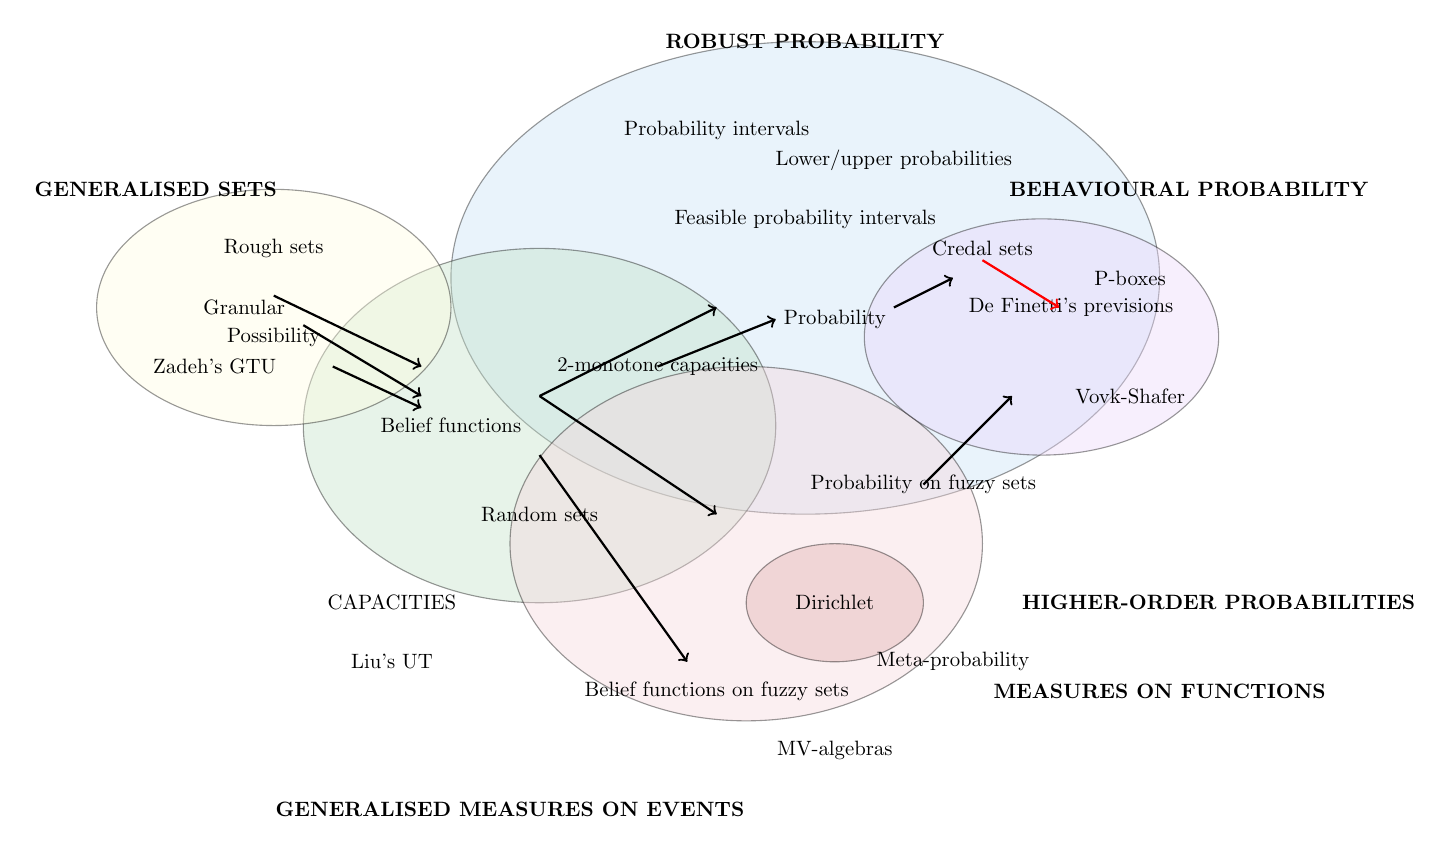
\begin{tikzpicture}[scale=0.75, every node/.style={scale=0.75}]

    % Colors
    \definecolor{bluearea}{RGB}{200,225,245}
    \definecolor{greenarea}{RGB}{195,225,200}
    \definecolor{yellowarea}{RGB}{255,253,225}
    \definecolor{redarea}{RGB}{245,215,220}
    \definecolor{purplearea}{RGB}{235,215,250}
    \definecolor{darkredarea}{RGB}{225,175,175}
    
    % Ellipses
    \draw[fill=bluearea,opacity=.4] (4,4.5) ellipse (6cm and 4cm);
    \draw[fill=greenarea,opacity=.4] (-0.5,2) ellipse (4cm and 3cm);
    \draw[fill=yellowarea,opacity=.4] (-5,4) ellipse (3cm and 2cm);
    \draw[fill=redarea,opacity=.4] (3,0) ellipse (4cm and 3cm);
    \draw[fill=purplearea,opacity=.4] (8,3.5) ellipse (3cm and 2cm);
    \draw[fill=darkredarea,opacity=.4] (4.5,-1) ellipse (1.5cm and 1cm);
    
    % Nodes (Texts)
    % Robust Probability
    \node at (4,8.5) {\textbf{ROBUST PROBABILITY}};
    \node at (2.5,7) {Probability intervals};
    \node at (5.5,6.5) {Lower/upper probabilities};
    \node at (4,5.5) {Feasible probability intervals};
    \node at (7,5) {Credal sets};
    \node at (9.5,4.5) {P-boxes};
    \node at (4.5,3.8) {Probability};
    
    % Generalised Sets
    \node at (-7,6) {\textbf{GENERALISED SETS}};
    \node at (-5,5) {Rough sets};
    \node at (-5.5,4) {Granular};
    \node at (-5,3.5) {Possibility};
    \node at (-6,3) {Zadeh's GTU};
    
    % Capacities
    \node at (-3,-1) {CAPACITIES};
    \node at (-2,2) {Belief functions};
    \node at (-0.5,0.5) {Random sets};
    \node at (-3,-2) {Liu's UT};
    \node at (1.5,3) {2-monotone capacities};
    
    % Behavioural Probability
    \node at (10.5,6) {\textbf{BEHAVIOURAL PROBABILITY}};
    \node at (8.5,4) {De Finetti's previsions};
    \node at (9.5,2.5) {Vovk-Shafer};
    
    % Measures on Functions
    \node at (10,-2.5) {\textbf{MEASURES ON FUNCTIONS}};
    \node at (6,1) {Probability on fuzzy sets};
    \node at (4.5,-1) {Dirichlet};
    \node at (6.5,-2) {Meta-probability};
    \node at (2.5,-2.5) {Belief functions on fuzzy sets};
    \node at (4.5, -3.5) {MV-algebras};
    
    \node at (11,-1) {\textbf{HIGHER-ORDER PROBABILITIES}};
    
    % Generalised measures on events
    \node at (-1,-4.5) {\textbf{GENERALISED MEASURES ON EVENTS}};
    
    % Arrows
    \draw[->,thick] (-4,3) -- (-2.5,2.3);
    \draw[->,thick] (-4.5,3.7) -- (-2.5,2.5);
    \draw[->,thick] (-5,4.2) -- (-2.5,3);
    \draw[->,thick] (-0.5,2.5) -- (2.5,4);
    \draw[->,thick] (-0.5,2.5) -- (2.5,0.5);
    \draw[->,thick] (-0.5,1.5) -- (2,-2);
    \draw[->,thick] (1.5,3) -- (3.5,3.8);
    \draw[->,thick] (5.5,4) -- (6.5,4.5);
    \draw[->,thick] (6,1) -- (7.5,2.5);
    \draw[->,thick,red] (7,4.8) -- (8.3,4);
    
    \end{tikzpicture}

\section{Structure of this work}







\chapter{Fuzzy Set Theory}
This chapter draws upon foundational concepts and theoretical frameworks presented in \cite{FULLER1} and \cite{FULLER2}. 
% \section*{Motivation}
% Fuzzy sets were introduced by Zadeh in 1965 \cite{Zadeh1965}. 
% \signal{the example of tall people, we want to model imprecision and why probability theory is not well suited for this. También pensar si voy a diferenciar entre incertidumbre epistemológica o aleatoria, o si eso lo meto cuando hable de possibility.}

\section{Fuzzy Sets}
Fuzzy sets were introduced by Zadeh in 1965, following the idea of generalizing sets that was presented in section \ref{sec:sorites}:

\say{More often than not, the classes of objects encountered in the real physical world do not have precisely defined criteria of membership. [...]Clearly, the ''class of all real numbers which are much greater than 1," or ''the class of beautiful women," or ''the class of tall men," do not constitute classes or sets in the usual mathematical sense of these terms. [...]Yet, the fact remains that such imprecisely defined ''classes" play an important role in human thinking, particularly in the domains of pattern recognition, communication of information, and abstraction.}\cite{Zadeh1965}\\

The idea he proposed for representing those classes is using a continuum of grades of membership. While classical (also called crisp or boolean) sets use a boolean membership function $\chi_A:X\rightarrow\{0,1\}$ that assigns either 0 or 1 to each element, fuzzy sets generalize this by using a membership function $\mu_A:X\rightarrow[0,1]$ that can assign any value between 0 and 1. 

\begin{remark}
    The membership degrees represent how compatible an object is with a set. Since membership degrees are real numbers in $[0,1]$, they are totally ordered. However, this does not imply a total ordering of objects, since two different objects may have the same membership degree. The set of objects can be totally ordered by considering equivalence classes of objects with the same membership degree.
\end{remark}

Let us take a closer look at Zadeh's example of the set of ''tall men" to answer a fundamental question: where do these membership values come from?

Most people would agree that a person with a height of 1.50m is not tall, so we can anchor the function with $\mu_{tall}(1.50) = 0$. Conversely, a person 2.00m tall is generally considered tall, so $\mu_{tall}(2.00) = 1$. But how should we define the values in between? The choice is not unique, and this non-uniqueness is not a flaw, but a feature.

However, not all choices are valid. For a membership function to be a reasonable model of ''tallness", it must be consistent with our understanding of the concept. For example, it would be illogical to define a 1.70m person as ''more tall" than a 1.80m person. This means the function must be non-decreasing. Furthermore, a classical boolean definition fails to capture the gradual nature of ''tallness", even if it is not \emph{wrong}, it lacks the expressive power for more a nuanced definition. Figure \ref{fig:tall_definitions} illustrates these points.

\begin{figure}[!ht]
    \centering
    \includegraphics[width=\textwidth]{ch1/figures/Fuzzy_tall.png}
    \caption{Illustrations of different membership functions for the fuzzy set ''tall". The left plot shows incorrect definitions: a crisp set is too rigid to capture the gradual nature of the concept, and a non-monotonic function is logically inconsistent since it implies a shorter person could be considered ''more tall" than a taller one. The right plot shows several valid, monotonic functions that can represent ''tall". Each reflects a different modeling choice, but all are anchored to the clear cases: membership is 0 for heights below 1.5m and 1 for heights above 2.0m.}
    \label{fig:tall_definitions}
\end{figure}

As shown in Figure \ref{fig:tall_correct}, there are infinitely many valid ways to define the fuzzy set ''tall". This flexibility might seem like a problem of subjectivity or a lack of rigor, but it is better understood as a \textbf{matter of definition}. In classical set theory, we don't ask whether the set of ''prime numbers" is more correct than the set of ''even numbers"; they are simply different sets defined for different purposes. 

Similarly, choosing a membership function \emph{is} the act of defining the fuzzy set. The goal is not to discover a single, universal truth for ''tallness," but to \textbf{design a fuzzy set that is useful for a specific problem}. This allows us to encode context-dependent or domain-specific expert knowledge into a precise mathematical model. The various methods for systematically creating these membership functions, a process known as \textit{fuzzification}, will be discussed in Section \ref{sec:fuzzification}.

For the remainder of this chapter, we will assume that appropriate fuzzy sets are given, and we will focus on the mathematical properties and operations that can be derived from them.


Therefore, fuzzy sets can be seen as an extension of crisp sets, since every crisp set can be modeled as a fuzzy set but not the other way around. The formal definition is as follows:

\begin{definition}[Fuzzy Set]
    Let $X\neq\emptyset$ a set. Then we define a \textbf{fuzzy set A in X}, i.e., $A \in \fuzzy{X}$ as:
    \[A=\{(x,\mu_A(x))\mid x\in X\}\]
    Where $\mu_A:X\longrightarrow [0,1]$ is the \textbf{membership function} and $X$ is the \textbf{domain} of the fuzzy set.
\end{definition}

\begin{remark}
     Both the fuzzy set and the membership function uniquely identify each other.
\end{remark}

\begin{notation}{Notation}
    We may use \( A(x) \equiv \mu_A(x) \) interchangeably.

    In general, $\chi$ will denote boolean membership functions and $\mu$, fuzzy membership functions.
\end{notation}



\begin{definition}[Support]
    Let $A \in \fuzzy{X}$. The crisp set of non zero membership value elements is called the support:
    \[\textnormal{Supp}(A)=\{x\in X \mid A(x)>0\}\]
\end{definition}

\begin{definition}[Fuzzy Subset]
    Given the fuzzy sets $A, B \in \fuzzy{X}$ we say $A$ is a fuzzy subset of $B$ (and write $A \subseteq B$) if and only if $A(x)
    \leq B(x) \forall x \in X$.

    Analogously, $A$ and $B$ are equal if and only if $A(x)=B(x) \forall x \in X$, i.e., each of them is a subset of the other.
\end{definition}

\begin{example}
    Here are some examples of common fuzzy sets:
    \begin{itemize}
        \item \textbf{Empty Fuzzy Set in $X$:} such that $\emptyset(x)=0 \forall x \in X$.
        \item \textbf{Universal Fuzzy Set in $X$:} such that $X(x)=1  \forall x \in X$.
        \item \textbf{Fuzzy Point in $X$:} such that $P(x_0)=1 \land A(x)=0 \forall x \in X-\{x_0\}$
        \item \textbf{Fuzzy Number:} Usually defined as a fuzzy set in $\mathbb{R}$ with some desirable properties. Will be covered in Section \ref{sec:fuzzy_numbers}.
    \end{itemize}
\end{example}

\section{Union, Intersection and Complement of Fuzzy Sets}
% \begin{notation}[label={not:OpsFS}]{Notation for variables in the current section}
%     In this section, we use the variable \( x \) to represent time and \( y \) to represent distance.
%   \end{notation}

The notions of union and intersection in fuzzy sets were first introduced by Zadeh \cite{Zadeh1965} using the operations $\max\{A(x),B(x)\}$ and $\min\{A(x),B(x)\}$ respectively. These can be intuitively interpreted as follows: the union is the \textit{smallest} fuzzy set (having lowest membership values) that contains both sets, while the intersection is the \textit{biggest} fuzzy set (having highest membership values) that is contained by both sets.\\

However, these operations can be generalized by two broader classes of operators: triangular norms (for intersection) and triangular conorms (for union).

Triangular norms were first introduced by Karl Menger in 1942 \cite{OriginTNorms} in the context of probabilistic metric spaces. When generalizing distances between points to probability distributions (representing the probability that the distance is less than or equal to a given value), Menger defined an operation $T:\,[0,1]\times [0,1]\to [0,1]$ to preserve the triangular inequality. For points $x,y,z$ in a metric space with distance function $d(\cdot,\cdot)$, this operation satisfies:

\begin{equation}\label{eq:Ftriangle_inequality}
d(x, z) \leq d(x, y) + d(y, z) \quad \longrightarrow \quad F_{xz}(t + s) \geq T(F_{xy}(t), F_{yz}(s)) \quad \forall t,s \geq 0
\end{equation}

This inequality means that the probability of $d(x,z)$ being less than $t+s$ must be at least the t-norm of the probabilities that $d(x,y)<t$ and $d(y,z)<s$. Note the change from $\leq$ to $\geq$ in the inequality. This is consistent with \textit{larger} probabilities indicating \textit{smaller} distances are more likely.\\

Since this originated in the context of distances, the following properties were required for an operator to be a t-norm\footnote{Associativity and one identity were not originally proposed by Menger but were later added by Sklar and Schweizer \cite{Sklar1983} in their refinement of triangular norms}:

\begin{itemize}
  \item \textbf{Symmetry:} The order of combining probabilities shouldn't matter, just as intersection of sets is commutative. That is, combining probabilities for distances $(x,y)$ and $(y,z)$ should give the same result regardless of order.
  
  \item \textbf{Associativity:} When combining multiple probabilities (e.g., for paths through points $x,y,z,w$), the grouping shouldn't affect the result. This extends the triangular norm to be consistent with polygonal inequalities, similar to how nested intersections satisfy $(A \cap B) \cap C = A \cap (B \cap C)$.
  
  \item \textbf{Monotonicity:} If the probability $F_{xy}(t)$ increases, then the lower bound for $F_{xz}(t+s)$ given by $T(F_{xy}(t), F_{yz}(s))$ should not decrease. This is analogous to how adding elements in crisp sets (or increasing membership degrees in fuzzy sets) cannot reduce the intersection set.
  
  \item \textbf{One Identity:} If $F_{yz}(s) = 1$ (meaning $d(y,z) < s$ with certainty), then $F_{xz}(t+s)$ depends only on $F_{xy}(t)$. This is analogous to how intersecting with the universal set preserves the original set.
\end{itemize}


% \say{The name \textit{triangular norm} refers to the fact that in the framework of probabilistic metric spaces, t-norms and t-conorms are used to generalize triangle inequality of ordinary metric spaces.}\cite{NGAN2018}\\

Therefore, the concept of intersection (conjunction) of fuzzy sets is generally represented by a triangular norm (also called a t-norm).

\begin{definition}[Triangular Norm]
    A mapping $T:[0,1]\times [0,1] \longrightarrow [0,1]$ that satisfies:
    \begin{romanenum}
      \item \textbf{Symmetricity:} $T(x,y) = T(y,x) \quad \oldforall x,y \in [0,1]$
      \item \textbf{Associativity:} $T(x,T(y,z)) = T(T(x,y),z) \quad \oldforall x,y,z \in [0,1]$
      \item \textbf{Monotonicity:} $T(x,y) \leq T(x',y') \quad \textnormal{if }x\leq x' \textnormal{ and } y\leq y' \quad \oldforall x,y,x',y' \in [0,1]$
      \item \textbf{One Identity:} $T(x,1) = T(1,x) = x \quad \oldforall x \in [0,1]$
    \end{romanenum}
    is called a triangular norm or t-norm. Defines the \textbf{intersection} of two fuzzy sets $A$ and $B$ on $X$ by giving the membership function as $(A \cap B) (x) = T(A(x),B(x)) \forall x \in X$ 
\end{definition}

Its dual operator can also be obtained by a similar reasoning as before, but instead of considering the probability distribution of finding both points closer than a given distance, it considers the probability distribution ($G_{uv}(t) = 1 - F_{uv}(t)$) of finding them further apart than that distance. In this case, both inequalities are $\leq$ since larger probabilities indicate that greater distances are more likely.
\begin{equation}\label{eq:Gtriangle_inequality}
d(x, z) \leq d(x, y) + d(y, z) \quad \longrightarrow \quad G_{xz}(t + s) \leq S(G_{xy}(t), G_{yz}(s))
\end{equation}

The reasoning regarding the properties is entirely analogous to the previous case, with the only difference being that $F_{uv}(t) = 1 \Leftrightarrow  G_{uv}(t) = 0$, and here the identity element is zero (union with the empty set).



\begin{definition}[Triangular Conorm]
  A mapping $S:[0,1]\times [0,1] \longrightarrow [0,1]$ that satisfies:
  \begin{enumerate}[(i)]\setlength{\itemindent}{2em}
    \item \textbf{Symmetricity:} $S(x,y) = S(y,x) \quad \oldforall x,y \in [0,1]$
    \item \textbf{Associativity:} $S(x,S(y,z)) = S(S(x,y),z) \quad \oldforall x,y,z \in [0,1]$
    \item \textbf{Monotonicity:} $S(x,y) \leq S(x',y') \quad \textnormal{if }x\leq x' \textnormal{ and } y\leq y' \quad \oldforall x,y,x',y' \in [0,1]$
    \item \textbf{Zero Identity:} $S(x,0) = S(0,x) = x \quad \oldforall x \in [0,1]$
  \end{enumerate}
  is called a triangular conorm or t-conorm. Defines the \textbf{union} of two fuzzy sets $A$ and $B$ on $X$ by giving the membership function as $(A \cup  B) (x) = S(A(x),B(x)) \forall x \in X$ 
    
\end{definition}

Complement was defined by Zadeh \cite{Zadeh1965} as\footnote{This is not the only definition that satisfies the axioms of a complement and is compatible with the classical limit, but it is the simplest one and will be used in this text. Other alternatives and their axioms can be found in \cite{Sladoje2007}. In \cite{Klement2000}, this is called the standard negation $N_s$.}:

\begin{definition}[Complement]
  The complement of a fuzzy set $A\in \fuzzy{X}$ is another fuzzy set with membership function given by $^\lnot A(x) \coleq 1 - A(x) \forall x\in X$
\end{definition}

Notice that this definition of complement is consistent with the classical definition of complement but implies that an element might have \textbf{non-zero partial membership} to both a fuzzy set and its complement: Let $A$ be a fuzzy set on $X$ and $x \in X / A(x)\notin \{0,1\}$ then $\lnot A(x)= 1 - A(x) \notin \{0,1\}$.\\

One consequence of this fact is that the union of a fuzzy set and its complement is not the total set in general. Analogously, the intersection will not the empty set in general. Those two properties that hold in classical sets but might not be true in fuzzy sets, are often called the \textbf{laws of excluded middle and of non-contradiction}, respectively.\\

However, there are t-norms and t-conorms such as the ones named after \luka that do satisfy both laws\footnote{Indeed, all continuous t-norms in agreement with non-contradiction are isomorphic to \luka \cite[p.~7]{LukasiewiczNonContrad}.}. Another example is the drastic t-norm which also satisfies the law of non-contradiction, but not the law of excluded middle. See example \ref{ex:basic_tnorms} for their formal expressions. \signal{All of this, has implications for the derived logic that will be explained in section \ref{sec:fuzzy_logic}. }\\

Another important property that classical union and intersection satisfy is De Morgan's Laws. For an arbitrary pair of t-norm and t-conorm, these laws are not automatically satisfied. However, there are specific pairs that do fulfill them. To illustrate the relationship between t-norms and t-conorms that satisfy De Morgan's Laws, we can use our probabilistic metric space analogy. Reconsidering the probabilistic metrics $F,G$ introduced earlier and substituting $F = 1 - G$ into equation \ref{eq:Ftriangle_inequality}, we obtain:

\[ G_{xz}(t + s) \leq 1 - T(1 - G_{xy}(t), 1 - G_{yz}(s))\]

Comparing this with equation \ref{eq:Gtriangle_inequality}, we can derive a relationship between t-norms and t-conorms, which is formalized in the following proposition:

\begin{proposition}[Relationship between t-norm and t-conorm]
  Given a t-norm $T$, the t-conorm is $S(a,b)\coleq 1 - T(1-a, 1-b)$ if and only if the union and intersection defined by that pair satisfy the De Morgan's Laws.
\end{proposition}
\begin{remark}
  It is easy to see that the previous relation is equivalent to $T(a,b) = 1-S(1-a, 1-b)$ which can be obtained simply by substituting $a'=1-a$ and $b'=1-b$, i.e., working with the complementary fuzzy sets.
\end{remark}

\begin{proof}
  Let $x\in X$, $A$, $B$ be fuzzy sets over $X$ with $a \coleq A(x)$ and $b \coleq B(x)$\\

  $\quad \boxed{\text{not}(A \text{ or } B) = (\text{not } A) \text{ and } (\text{not } B)}$\\
  [0.5em]
  $\lnot S(a,b) = T(\lnot a, \lnot b) \iff 1 - S(a,b) = T(1-a, 1-b) \iff S(a,b) = 1 - T(1-a, 1-b)$\\

  $\quad \boxed{\text{not}(A \text{ and } B) = (\text{not } A) \text{ or } (\text{not } B)}$\\
  [0.5em]
  $\lnot T(a,b) = S(\lnot a, \lnot b) \iff 1 - T(a,b) = S(1-a, 1-b) \iff T(a,b) = 1 - S(1-a, 1-b)$

\end{proof}

\signal{Creo que además de esto de las leyes de de Morgan, también nos da que el modus ponen funciona si se cumple la propiedad esa. Además no sé si se llama residual property.}

\signal{
  Lo de archimedean sirve para el teorema 1.8.1 de \cite{FULLER2}. Y tb con la law of large numbers con LR-fuzzy numbers.}



  \subsection{Classification of T-norms}

\signal{Añadir lo de strict archimedean y divisores de zero y eso.}
\begin{definition}[Archimedean t-norm]
  A continuous t-norm that satisfies $T(x,x)<x \forall x\in ]0,1[$ is called an archimedean t-norm.
\end{definition}

\begin{proposition}[Characterization of archimedean t-norms]
  For all archimedean t-norms there exists a continuous decreasing function $f:[0,1] \longrightarrow [0,\infty[$ with $f(1)=0$ such that: 
  \[ 
  T(x,y)= f^{-1}(\min\{f(x)+f(y), f(0)\}) \text{ where } f^{-1} =
  \begin{cases}
    f^{-1}(y) & \text{if } y\in [0,f(0) ]\\
    0 & \text{otherwise}
  \end{cases}
  \text{ is a pseudo-inverse}.
  \]
\end{proposition}


\signal{
\begin{definition}[Nilpotent t-norm]
  
\end{definition}}

\begin{definition}[Weaker t-norm]
  Given $T_1, T_2$ t-norms, then $T_1$ is weaker than $T_2$ $(T_1 \leq T_2)$ if $T_1(x,y)\leq T_2(x,y)\forall x,y\in [0,1]$.\\
  In that case, it is equivalent to say $T_2$ is stronger than $T_1$ $(T_2 \geq T_1)$

\end{definition}
\begin{remark}
  This defines a partial order relation in the set of t-norms.
\end{remark}
\signal{The weaker the t-norm, the stronger the associated s-norm. Lo pongo como un remark igual.}

\signal{
There are many results like all t-norms are between the weak and the min, all t-conorms are between max and strong, or that min is the only t-norm that satisfies $T(a,a)=a$ (igual es por esto ultimo q se usa tanto. Qué implicaciones tiene que lukasiewicz no cumpla eso?)}

\signal{Tambien lo de que la T-norm e distributiva con max/sup sirve para justificar la definicion del producto cartesiano, así que esa propiedad la tendré que meter por aquí igual.}


\noindent\rule{\textwidth}{2pt}


\subsection{Basic Properties and Examples of T-norms}
The set of all t-norms can be partially ordered, which helps in their classification.
\begin{definition}[Weaker/Stronger t-norm {\cite[Def.~1.4]{Klement2000}}]
  Given two t-norms $T_1$ and $T_2$, $T_1$ is said to be \emph{weaker} than $T_2$ (denoted $T_1 \leq T_2$) if $T_1(x,y) \leq T_2(x,y) \forall x,y \in [0,1]$.
  Equivalently, $T_2$ is said to be \emph{stronger} than $T_1$.
\end{definition}
\begin{remark}
  The relation $\leq$ defines a partial order on the set of all t-norms. It's a fundamental result that for any t-norm $T$, we have $T_D \leq T \leq T_M$, where $T_D$ is the drastic product and $T_M$ is the minimum t-norm (\cite[Rem.~1.5]{Klement2000}).
\end{remark}
In order to classify t-norms further, the following algebraic properties will be needed \cite[Def.~2.1]{Klement2000}:
\begin{definition}[Idempotent Element]
Let $T$ be a t-norm. An element $a \in [0,1]$ is an \emph{idempotent element} of $T$ if $T(a,a)=a$. The elements $0$ and $1$ are always trivial idempotent elements.
\end{definition}

\begin{definition}[Nilpotent Element]
Let $T$ be a t-norm. An element $a \in ]0,1[$ is a \emph{nilpotent element} of $T$ if there exists $n \in \mathbb{N}$ such that $a_T^{(n)} = 0$, where $a_T^{(n)} = T(a, a_T^{(n-1)})$ with $a_T^{(1)}=a$.
\end{definition}

\begin{definition}[Zero Divisor]
Let $T$ be a t-norm. An element $a \in ]0,1[$ is a \emph{zero divisor} of $T$ if there exists $b \in ]0,1[$ such that $T(a,b)=0$.
\end{definition}

\begin{definition}[Archimedean T-norm]
A t-norm $T$ is \emph{Archimedean} if for each $(x,y) \in ]0,1[^2$ there is an $n \in \mathbb{N}$ with $x_T^{(n)} < y$ (\cite[Def.~2.9]{Klement2000}). 

Equivalently, a continuous t-norm $T$ is Archimedean if and only if $T(x,x) < x \forall x \in ]0,1[$ (\cite[Thm.~2.12]{Klement2000}). 
\end{definition}

\begin{example}[Basic T-norms {\cite[Ex.~1.2]{Klement2000}}]
  
  \begin{itemize}
    \item \textbf{Minimum ($T_M$):} $T_M(x, y) = \min(x, y)$.
    This is the strongest t-norm (\cite[Rem.~1.5(i)]{Klement2000}). Every element $x \in [0,1]$ is an idempotent element ($T_M(x,x)=x$). It is not Archimedean (unless interpreted on a trivial interval, as it has non-trivial idempotents). It has no zero divisors and no nilpotent elements other than 0.
    \item \textbf{Product ($T_P$):} $T_P(x, y) = x \cdot y$.
    This t-norm is strict Archimedean (\cite[Ex.~2.14(i)]{Klement2000}). It has only $0$ and $1$ as idempotent elements, no nilpotent elements (other than $0$), and no zero divisors (\cite[Ex.~2.2(i)]{Klement2000}).
    \item \textbf{Łukasiewicz ($T_L$):} $T_L(x, y) = \max(0, x + y - 1)$.
    This t-norm is nilpotent Archimedean (\cite[Ex.~2.14(i)]{Klement2000}). It has only $0$ and $1$ as idempotent elements. Every $a \in ]0,1[$ is a nilpotent element and also a zero divisor (\cite[Ex.~2.2(i)]{Klement2000}).
    \item \textbf{Drastic Product ($T_D$):} $T_D(x, y) = \begin{cases} \min(x,y) & \text{if } \max(x,y)=1 \\ 0 & \text{otherwise} \end{cases}$.
    This is the weakest t-norm (\cite[Rem.~1.5(i)]{Klement2000}). It is Archimedean since $T_D(x,x)=0 < x$ for $x \in ]0,1[$. It has only $0$ and $1$ as idempotent elements. Every $a \in ]0,1[$ is a zero divisor, and also nilpotent (since $a_D^{(2)} = T_D(a, T_D(a,a)) = T_D(a,0) = 0$ for $a<1$). It is not continuous.
  \end{itemize}
\end{example}

\subsection{Classification of Continuous T-norms}
\signal{Add an appendix with upper, lower, left, right continuity.}

Continuous t-norms form a particularly well-structured class, admitting elegant representation theorems. Their study often revolves around whether they are Archimedean.

\subsubsection{Continuous Archimedean T-norms and Generators}
The structure of continuous Archimedean t-norms is intimately linked to certain functions called generators.
\begin{definition}[Additive Generator and Pseudo-inverse]
  An \emph{additive generator} of a t-norm $T$ is a strictly decreasing function $t: [0,1] \to [0,\infty]$ which is right-continuous in $0$ and satisfies $t(1)=0$, such that $T(x,y) = t^{(-1)}(t(x) + t(y))$ for all $(x,y) \in [0,1]^2$, provided $t(x)+t(y) \in \mathrm{Ran}(t) \cup [t(0),\infty]$ (\cite[Def.~3.25, p.~70]{Klement2000}).
  The function $t^{(-1)}: [0,\infty] \to [0,1]$ is the \emph{pseudo-inverse} of $t$, defined as $t^{(-1)}(y) = \sup \{ x \in [0,1] \mid t(x) > y \}$ (adapted from \cite[Def.~3.2, p.~68 and Cor.~3.3]{Klement2000} for strictly decreasing $t$). \signal{`Ran(t)` denotes the range of $t$, i.e., the set of all values $t(x)$ for $x \in [0,1]$ \cite[p. xvii]{Klement2000}.}
\end{definition}

\begin{theorem}[Representation of Continuous Archimedean T-norms {\cite[Thm.~5.1, p.~122]{Klement2000}}]
  A t-norm $T$ is a continuous Archimedean t-norm if and only if it possesses a continuous additive generator $t: [0,1] \to [0,\infty]$. This generator is unique up to a positive multiplicative constant.
\end{theorem}
Continuous Archimedean t-norms are further categorized based on the behavior of their generator at $0$:
\begin{itemize}
    \item $T$ is \textbf{strict} if its continuous additive generator $t$ satisfies $t(0)=\infty$. This means $T(x,y)>0$ whenever $x,y > 0$. Strict t-norms are strictly monotone on $]0,1]^2$. (\cite[Cor.~3.30(i), p.~88; Def.~2.13(i), p.~42]{Klement2000}).
    \item $T$ is \textbf{nilpotent} if its continuous additive generator $t$ satisfies $t(0)<\infty$. This implies that for any $x,y \in ]0,1[$, there exists $n$ such that $T(x, \dots, x)$ ($n$ times) is $0$. Every $a \in ]0,1[$ is a nilpotent element. (\cite[Cor.~3.30(ii), p.~88; Def.~2.13(ii), p.~42]{Klement2000}).
\end{itemize}

\subsubsection{Isomorphism of Continuous Archimedean T-norms}
The concept of isomorphism reveals a deep structural similarity among t-norms within these classes.
\begin{definition}[Isomorphic T-norms {\cite[Def.~2.27, p.~51; Prop.~2.28(iv), p.~52]{Klement2000}}]
  Two t-norms $T_1$ and $T_2$ are \emph{isomorphic} if there exists a strictly increasing bijection $\varphi: [0,1] \to [0,1]$ (an automorphism of the unit interval) such that $T_2(x,y) = \varphi^{-1}(T_1(\varphi(x), \varphi(y)))$ for all $x,y \in [0,1]$.
\end{definition}
Isomorphic t-norms share the same algebraic structure, merely operating on rescaled inputs and outputs via $\varphi$. A fundamental result is:
\begin{proposition}[{\cite[Cor.~5.7, p.~125, referring to Prop.~5.9 and Prop.~5.10]{Klement2000}}]
  \begin{enumerate}
      \item Every strict t-norm is isomorphic to the Product t-norm $T_P$.
      \item Every nilpotent t-norm is isomorphic to the Łukasiewicz t-norm $T_L$.
  \end{enumerate}
\end{proposition}
This implies that, up to isomorphism, there are only two distinct types of continuous Archimedean t-norms: the product type and the Łukasiewicz type.

\subsubsection{General Continuous T-norms and Ordinal Sums}
Continuous t-norms that are not Archimedean must have non-trivial idempotent elements. These are constructed using ordinal sums.
\begin{definition}[Ordinal Sum of T-norms {\cite[Def.~3.44, p.~97]{Klement2000}}]
Let $(T_\alpha)_{\alpha \in A}$ be a family of t-norms and $(]a_\alpha, e_\alpha[)_{\alpha \in A}$ be a family of non-empty, pairwise disjoint open subintervals of $[0,1]$. The t-norm $T$ defined by
\[
T(x,y) =
\begin{cases}
  a_\alpha + (e_\alpha - a_\alpha) \cdot T_\alpha \left( \frac{x-a_\alpha}{e_\alpha - a_\alpha}, \frac{y-a_\alpha}{e_\alpha - a_\alpha} \right) & \text{if } (x,y) \in [a_\alpha, e_\alpha]^2 \text{ for some } \alpha \in A \\
  \min(x,y) & \text{otherwise}
\end{cases}
\]
is called the \emph{ordinal sum} of the summands $(a_\alpha, e_\alpha, T_\alpha)$, $\alpha \in A$.
\end{definition}
Intuitively, an ordinal sum "glues" copies of the t-norms $T_\alpha$ (scaled to fit the intervals $[a_\alpha, e_\alpha]$) onto the diagonal of the unit square. Outside these "active" regions, the t-norm behaves like the minimum $T_M$. The endpoints $a_\alpha, e_\alpha$ become idempotent elements of $T$.

\begin{theorem}[Representation of Continuous T-norms {\cite[Thm.~5.11, p.~140]{Klement2000}}]
  A function $T: [0,1]^2 \to [0,1]$ is a continuous t-norm if and only if $T$ is uniquely representable as an ordinal sum of continuous Archimedean t-norms.
\end{theorem}
\begin{remark}
  A continuous t-norm is \emph{ordinally irreducible} if its only ordinal sum representation is $T = ((0,1,T))$. For continuous t-norms, being ordinally irreducible is equivalent to being Archimedean (\cite[Prop.~3.53, p.~99 and context]{Klement2000}). Thus, the "building blocks" in the ordinal sum representation are precisely the continuous Archimedean t-norms (isomorphic to $T_P$ or $T_L$). If the family of subintervals is empty, the ordinal sum is defined as $T_M$.
\end{remark}

\subsection{Further Examples: Parametric Families of T-norms}
Beyond the four basic t-norms, several parametric families offer a spectrum of behaviors and are widely used. Their construction often relies on generators.
\begin{definition}[Multiplicative Generator {\cite[Def.~3.36, p.~91]{Klement2000}}]
  A \emph{multiplicative generator} $\theta: [0,1] \to [0,1]$ of a t-norm $T$ is a strictly increasing function, right-continuous in $0$, with $\theta(1)=1$, such that $T(x,y) = \theta^{(-1)}(\theta(x) \cdot \theta(y))$, assuming $\theta(x)\cdot\theta(y)$ is in a suitable range. \signal{This is a simplified statement; the book's definition includes range conditions.}
\end{definition}
\begin{remark}[Duality of Generators {\cite[Rem.~3.34, p.~90]{Klement2000}}]
  If $t(x)$ is an additive generator, then $\theta(x) = e^{-c \cdot t(x)}$ (for some $c>0$) is a multiplicative generator, and if $\theta(x)$ is a multiplicative generator, then $t(x) = -c \cdot \log(\theta(x))$ is an additive generator.
\end{remark}

\begin{example}[Parametric Families of T-norms (selected from {\cite[Chapter 4]{Klement2000}})]
  \begin{itemize}
    \item \textbf{Schweizer-Sklar T-norms ($T_\lambda^{SS}$), $\lambda \in [-\infty, \infty]$:}
    $T_\lambda^{SS}(x,y) = (\max(0, x^\lambda + y^\lambda - 1))^{1/\lambda}$.
    Includes $T_M (\lambda=-\infty)$, $T_P (\lambda \to 0)$, $T_L (\lambda=1)$, $T_D (\lambda=\infty)$. Additive generator $t_\lambda^{SS}(x) = \frac{1-x^\lambda}{\lambda}$ for $\lambda \neq 0$.
    \item \textbf{Frank T-norms ($T_\lambda^F$), $\lambda \in [0, \infty]$:}
    $T_\lambda^F(x,y) = \log_\lambda \left(1 + \frac{(\lambda^x-1)(\lambda^y-1)}{\lambda-1}\right)$ for $\lambda \in ]0,\infty[, \lambda \neq 1$.
    Includes $T_M (\lambda=0)$, $T_P (\lambda=1)$, $T_L (\lambda=\infty)$. All $T_\lambda^F$ for $\lambda \in ]0,\infty]$ are continuous Archimedean. Additive generator $t_\lambda^F(x) = -\log \frac{\lambda^x-1}{\lambda-1}$.
    \item \textbf{Yager T-norms ($T_p^Y$), $p \in [0, \infty]$:} \signal{The book uses $\lambda$ for Yager, but $p$ is more common in literature to avoid clash with Frank's parameter.}
    $T_p^Y(x,y) = \max(0, 1 - ((1-x)^p + (1-y)^p)^{1/p})$ for $p \in ]0,\infty[$.
    Includes $T_D (p \to 0)$, $T_L (p=1)$, $T_M (p=\infty)$. All $T_p^Y$ for $p \in ]0,\infty[$ are continuous nilpotent Archimedean. Additive generator $t_p^Y(x) = (1-x)^p$.
  \end{itemize}
  \signal{Many other families exist, like Hamacher, Dombi, Aczél-Alsina, Sugeno-Weber, Mayor-Torrens. Refer to \cite[Table 4.1, p.~119]{Klement2000} and Appendix A therein for a comprehensive list and properties.}
\end{example}

\subsection{Non-Continuous T-norms and Left-Continuity}
While continuous t-norms are well-classified, not all t-norms are continuous.
The \textbf{drastic product $T_D$} is a key example of a non-continuous t-norm. It is Archimedean. It is upper semicontinuous, implying right-continuity in each variable when the other is fixed (\cite[Rem.~1.21(i), Prop.~1.22]{Klement2000}). However, it is not left-continuous (e.g., at $(1,y)$ for $y<1$).

The \textbf{nilpotent minimum $T^{nM}$} (\cite[Rem.~1.21(i), p.~16]{Klement2000}) is defined as:
  \[
  T^{nM}(x,y) =
  \begin{cases}
    0 & \text{if } x+y \leq 1 \\
    \min(x,y) & \text{otherwise.}
  \end{cases}
  \]
This t-norm is lower semicontinuous, which for monotone functions implies it is left-continuous in each variable (\cite[Prop.~1.22, p.~17]{Klement2000}). It is not continuous (specifically, not right-continuous at points on the line $x+y=1$ when approached from $x+y>1$).

The \textbf{Krause t-norm $T^K$} (\cite[App.~B.1, Thm.~B.1]{Klement2000}) is a more complex example. It is constructed using the Cantor set and Farey series. It is stated to be "neither left- nor right-continuous, but has a continuous diagonal section." This highlights that t-norms can exhibit quite irregular continuity behavior.

\begin{remark}[Importance of Left-Continuity]
For non-continuous t-norms, the property of \emph{left-continuity} (in each variable) is often a desirable, or even required, condition in certain applications, particularly in fuzzy logic. For instance, in residuum-based logics, if a t-norm $T$ is left-continuous, its corresponding residuated implication $I(x,y) = \sup\{z \in [0,1] \mid T(x,z) \le y\}$ exhibits well-behaved properties. Specifically, a commutative, integral lattice-ordered monoid based on $T$ is residuated if and only if $T$ is left-continuous (\cite[Prop.~2.47, p.~63]{Klement2000}). This ensures that the implication adequately captures deductive reasoning. While the intuitive notion that "a microscopic decrease of the truth degree of a conjunct should not macroscopically decrease the truth degree of the conjunction" points towards continuity, left-continuity is a weaker but often sufficient condition for preserving logical coherence in such frameworks.
\end{remark}


\noindent\rule{\textwidth}{2pt}


\subsection{Classification of T-norms}
\signal{Hablar de los generadores de las t-norms (familias) y propiedades. Diagrama de qué t-norms son weaker que otras. Cuáles son continuas y cuales no (drastic por ejemplo)}

\signal{Normalmente se pide que sean left continuous (it is sufficient in either argument \cite{Esteva2001MonoidalTB}), which expresses the assumption that a microscopic decrease of the truth degree of a conjunct should not macroscopically decrease the truth degree of conjunction.}

The set of all t-norms can be partially ordered, and understanding their properties allows for a useful classification, particularly for continuous t-norms.

\begin{definition}[Weaker/Stronger t-norm {\citep[Definition 1.4, p.~21]{Klement2000}}]
  Given two t-norms $T_1$ and $T_2$, $T_1$ is said to be \emph{weaker} than $T_2$ (denoted $T_1 \leq T_2$) if $T_1(x,y) \leq T_2(x,y)$ for all $x,y \in [0,1]$.
  Equivalently, $T_2$ is said to be \emph{stronger} than $T_1$.
\end{definition}

\begin{remark}
  The relation $\leq$ defines a partial order on the set of all t-norms.
  It's a fundamental result that for any t-norm $T$, we have $T_D \leq T \leq T_M$, where $T_D$ is the drastic product and $T_M$ is the minimum t-norm (\citep[Remark 1.5(i), p.~21]{Klement2000}).
\end{remark}

\begin{remark}
  Duality with t-conorms: If $T_1 \leq T_2$ are t-norms, and $S_1, S_2$ are their respective dual t-conorms (obtained via a strong negation $N$, typically $N(x)=1-x$), then $S_1 \geq S_2$. Thus, a weaker t-norm corresponds to a stronger dual t-conorm.
\end{remark}

To classify t-norms further, several algebraic properties are essential:

\begin{definition}[Algebraic Properties of T-norms {\citep[Definition 2.1, Definition 2.9]{Klement2000}}]
Let $T$ be a t-norm.
\begin{enumerate}
    \item An element $a \in [0,1]$ is an \emph{idempotent element} of $T$ if $T(a,a)=a$. The elements $0$ and $1$ are always trivial idempotent elements.
    \item An element $a \in ]0,1[$ is a \emph{nilpotent element} of $T$ if there exists $n \in \mathbb{N}$ such that $a_T^{(n)} = 0$, where $a_T^{(n)}$ denotes the $n$-th power of $a$ with respect to $T$.
    \item An element $a \in ]0,1[$ is a \emph{zero divisor} of $T$ if there exists $b \in ]0,1[$ such that $T(a,b)=0$.
    \item $T$ is \emph{Archimedean} if for each $(x,y) \in ]0,1[^2$ there is an $n \in \mathbb{N}$ with $x_T^{(n)} < y$. Equivalently, a t-norm $T$ is Archimedean if and only if it has only trivial idempotent elements (0 and 1) and satisfies a further condition related to limits, or more simply for continuous t-norms, if $T(x,x) < x$ for all $x \in ]0,1[$ (\citep[Theorem 2.12 and Theorem 5.1]{Klement2000}).
\end{enumerate}
\end{definition}

\begin{proposition}[{\citep[Proposition 1.9(i), p.~24]{Klement2000}}]
  The minimum t-norm $T_M(x,y) = \min(x,y)$ is the only t-norm $T$ satisfying $T(x,x)=x$ for all $x \in [0,1]$.
\end{proposition}

\paragraph{Continuous T-norms}
Continuous t-norms admit a very structured classification.

\begin{theorem}[Generator Theorem for Continuous Archimedean T-norms {\citep[Theorem 5.1, p.~122]{Klement2000}}]
  A function $T: [0,1]^2 \to [0,1]$ is a continuous Archimedean t-norm if and only if it has a \emph{continuous additive generator}. That is, there exists a continuous, strictly decreasing function $t: [0,1] \to [0,\infty]$ with $t(1)=0$, such that for all $(x,y) \in [0,1]^2$:
  \[
  T(x,y) = t^{(-1)}(t(x) + t(y))
  \]
  where $t^{(-1)}: [0,\infty] \to [0,1]$ is the pseudo-inverse of $t$, defined as
  \[
  t^{(-1)}(z) =
  \begin{cases}
    t^{-1}(z) & \text{if } z \in [0, t(0)] \\
    0 & \text{if } z \in ]t(0), \infty]
  \end{cases}
  \]
  (If $t(0)=\infty$, then $t^{(-1)} = t^{-1}$). The generator $t$ is unique up to a positive multiplicative constant.
\end{theorem}

Continuous Archimedean t-norms are further divided into two main classes:

\begin{definition}[Strict and Nilpotent T-norms {\citep[Definition 2.13, p.~42]{Klement2000}}]
  \begin{enumerate}
      \item A t-norm $T$ is called \emph{strict} if it is continuous and strictly monotone (i.e., $T(x,y) < T(x,z)$ whenever $x>0$ and $y<z$).
      \item A t-norm $T$ is called \emph{nilpotent} if it is continuous and if each $a \in ]0,1[$ is a nilpotent element of $T$.
  \end{enumerate}
\end{definition}

\begin{corollary}[{\citep[Corollary 3.30, p.~88]{Klement2000}}]
  Let $T$ be a continuous Archimedean t-norm with a continuous additive generator $t$.
  \begin{enumerate}
      \item $T$ is strict if and only if $t(0) = \infty$.
      \item $T$ is nilpotent if and only if $t(0) < \infty$.
  \end{enumerate}
\end{corollary}

\begin{proposition}[Isomorphism of Continuous Archimedean T-norms {\citep[Corollary 5.7, p.~125; Proposition 5.9, p.~126; Proposition 5.10, p.~127]{Klement2000}}]
  \begin{enumerate}
      \item Every strict t-norm is isomorphic to the product t-norm $T_P(x,y) = xy$.
      \item Every nilpotent t-norm is isomorphic to the Łukasiewicz t-norm $T_L(x,y) = \max(0, x+y-1)$.
  \end{enumerate}
  This means that any continuous Archimedean t-norm is isomorphic to either $T_P$ or $T_L$.
\end{proposition}

\paragraph{Ordinal Sum Representation}
Not all continuous t-norms are Archimedean. Those that are not (i.e., possess non-trivial idempotents) can be constructed from Archimedean t-norms using the concept of an ordinal sum.

\begin{definition}[Ordinal Sum of T-norms {\citep[Definition 3.44, p.~97]{Klement2000}}]
Let $(T_\alpha)_{\alpha \in A}$ be a family of t-norms and $(]a_\alpha, e_\alpha[)_{\alpha \in A}$ be a family of non-empty, pairwise disjoint open subintervals of $[0,1]$. The t-norm $T$ defined by
\[
T(x,y) =
\begin{cases}
  a_\alpha + (e_\alpha - a_\alpha) \cdot T_\alpha \left( \frac{x-a_\alpha}{e_\alpha - a_\alpha}, \frac{y-a_\alpha}{e_\alpha - a_\alpha} \right) & \text{if } (x,y) \in [a_\alpha, e_\alpha]^2 \text{ for some } \alpha \in A \\
  \min(x,y) & \text{otherwise}
\end{cases}
\]
is called the \emph{ordinal sum} of the summands $(a_\alpha, e_\alpha, T_\alpha)$, $\alpha \in A$.
We denote this as $T = ((a_\alpha, e_\alpha, T_\alpha))_{\alpha \in A}$.
\end{definition}

\begin{theorem}[Representation of Continuous T-norms {\citep[Theorem 5.11, p.~140]{Klement2000}}]
  A function $T: [0,1]^2 \to [0,1]$ is a continuous t-norm if and only if $T$ is uniquely representable as an ordinal sum of continuous Archimedean t-norms.
\end{theorem}

\begin{remark}
  A t-norm is \emph{ordinally irreducible} if it only has a trivial ordinal sum representation (i.e., $T = ((0,1,T))$). For continuous t-norms, being ordinally irreducible is equivalent to being Archimedean (\citep[Proposition 3.53, p.~99]{Klement2000}).
\end{remark}

In summary, continuous t-norms are either Archimedean (and thus isomorphic to $T_P$ or $T_L$) or they are ordinal sums of such Archimedean t-norms (and $T_M$ as a limiting case).





\begin{example}
  \signal{Some examples of t-norms and t-conorms.}
  \begin{itemize}
    \item \textbf{Minimum/Maximum:} 
    The strongest t-norm (minimum) and weakest t-conorm (maximum). They are the standard interpretations of conjunction and disjunction in fuzzy logic and are idempotent ($T(x,x)=x, S(x,x)=x$).\\
    $T_M(x, y) = \min(x, y) \quad S_M(x, y) = \max(x, y)$

    \item \textbf{Łukasiewicz:}
    Represents a bounded arithmetic sum/difference logic. Corresponds to the logic introduced by Łukasiewicz. It is Archimedean but not strict (has zero divisors). Boundary condition for t-norms satisfying $T(x,y)+S(x,y) = x+y$. \\
    $T_L(x, y) = \max(0, x + y - 1) \quad S_L(x, y) = \min(1, x + y)$

    \item \textbf{Product:}
    The standard algebraic product t-norm and the probabilistic sum t-conorm. Represents the intersection of independent events in probability theory. It is a strict Archimedean t-norm. \\
    $T_P(x, y) = x \cdot y \quad S_P(x, y) = x + y - x \cdot y$

    \item \textbf{Drastic:}
    The weakest t-norm and the strongest t-conorm. They represent the most extreme intersection and union possible. \signal{Discontinuous except at boundary points (0,0), (1,1), etc.} \\
    $T_D(x, y) = \begin{cases} \min(x,y) & \text{if } \max(x,y)=1 \\ 0 & \text{otherwise} \end{cases} \quad S_D(x, y) = \begin{cases} \max(x,y) & \text{if } \min(x,y)=0 \\ 1 & \text{otherwise} \end{cases}$
    % Simpler equivalent definitions:
    % T(x, y) = y if x=1, x if y=1, 0 otherwise
    % S(x, y) = y if x=0, x if y=0, 1 otherwise

    \item \textbf{Hamacher Family ($\gamma \ge 0$):}
    A parametric family of t-norms and t-conorms. Includes the Product t-norm as a special case when $\gamma = 1$. It is strictly Archimedean for $\gamma > 0$. \\
    $T_\gamma(x, y) = \frac{xy}{\gamma + (1-\gamma)(x+y-xy)} \quad S_\gamma(x, y) = \frac{x+y-xy-(1-\gamma)xy}{1-(1-\gamma)xy}$
    % Note: For gamma=0 this is related to Lukasiewicz via generator, for gamma -> infinity to Drastic.

    \item \textbf{Dubois and Prade Family ($\alpha \in [0, 1]$):}
    A parametric family that includes the Minimum t-norm ($\alpha=0$) and the Product t-norm ($\alpha=1$). Provides flexibility between these two important t-norms. \\
    $T_\alpha(x, y) = \frac{xy}{\max(x, y, \alpha)} \quad S_\alpha(x, y) = 1 - \frac{(1-x)(1-y)}{\max(1-x, 1-y, \alpha)}$ 
    % Note: The S-conorm is expressed directly via duality relation S(x,y) = 1 - T(1-x, 1-y).

    \item \textbf{Yager Family ($p > 0$):}
    A parametric family characterized by the parameter $p$. It approaches the Drastic t-norm as $p \to 0^+$ and the Minimum t-norm as $p \to \infty$. The Łukasiewicz t-norm is obtained for $p=1$. \\
    $T_p(x, y) = \max(0, 1 - ((1-x)^p + (1-y)^p)^{1/p}) \quad S_p(x, y) = \min(1, (x^p + y^p)^{1/p})$

    \item \textbf{Frank Family ($p > 0, p \neq 1$):}
    The only family of t-norms (besides min-max) that are Archimedean and satisfy the functional equation $T(x, y) + S(x, y) = x + y$. It includes Łukasiewicz ($p \to 0^+$), Product ($p \to 1$), and Minimum/Maximum ($p \to \infty$) as limiting cases. \\
    $T_p(x, y) = \log_p \left( 1 + \frac{(p^x - 1)(p^y - 1)}{p - 1} \right) \quad S_p(x, y) = 1 - \log_p \left( 1 + \frac{(p^{1-x} - 1)(p^{1-y} - 1)}{p - 1} \right)$

    \item \textbf{Schweizer-Sklar Family ($p \in [-\infty, \infty]$):}
    A very general parametric family encompassing several others. Includes Drastic ($p \to -\infty$), Łukasiewicz ($p=1$ in a different parameterization, not this T form), Product ($p=0$ in a related form), and Minimum ($p \to \infty$). The Yager family is generated differently but related. \\
    $T_p(x, y) = (\max(0, x^p + y^p - 1))^{1/p} \quad S_p(x, y) = 1 - (\max(0, (1-x)^p + (1-y)^p - 1))^{1/p}$ 
    % Note: S-conorm shown is the dual S_p(x,y) = 1 - T_p(1-x, 1-y). The commonly cited S_p(x,y) = (min(1, x^p + y^p))^{1/p} is NOT dual to this T_p w.r.t standard negation.
  \end{itemize}
\end{example}





\subsection{Construction and Properties of T-norms} % Example section

\subsubsection{Generators for T-norms}

One of the most powerful methods for constructing and characterizing t-norms, particularly continuous Archimedean ones, involves the use of generator functions.

\begin{definition}[Additive Generator {\cite[Definition 3.25, p.~70]{Klement2000}}]
  An \emph{additive generator} $t: [0,1] \to [0,\infty]$ of a t-norm $T$ is a strictly decreasing function which is also right-continuous in $0$ and satisfies $t(1)=0$, such that for all $(x,y) \in [0,1]^2$:
  \begin{enumerate}
      \item $t(x) + t(y) \in \mathrm{Ran}(t) \cup [t(0), \infty]$, and
      \item $T(x,y) = t^{(-1)}(t(x) + t(y))$,
  \end{enumerate}
  where $t^{(-1)}$ is the pseudo-inverse of $t$.
\end{definition}

\begin{remark}
  As established in \cite[Theorem 5.1, p.~122]{Klement2000}, every continuous Archimedean t-norm possesses a continuous additive generator, unique up to a positive multiplicative constant. Conversely, any such generator defines a continuous Archimedean t-norm.
\end{remark}

\begin{definition}[Multiplicative Generator {\cite[Definition 3.36, p.~91]{Klement2000}}]
  A \emph{multiplicative generator} $\theta: [0,1] \to [0,1]$ of a t-norm $T$ is a strictly increasing function which is right-continuous in $0$ and satisfies $\theta(1)=1$, such that for all $(x,y) \in [0,1]^2$:
  \begin{enumerate}
      \item $\theta(x) \cdot \theta(y) \in \mathrm{Ran}(\theta) \cup [0, \theta(0)]$, and
      \item $T(x,y) = \theta^{(-1)}(\theta(x) \cdot \theta(y))$,
  \end{enumerate}
  where $\theta^{(-1)}$ is the pseudo-inverse of $\theta$.
\end{definition}

\begin{remark}
  There is a direct duality between additive and multiplicative generators. If $t$ is an additive generator, then $\theta(x) = e^{-t(x)}$ (or $e^{-c \cdot t(x)}$ for $c>0$) can serve as a multiplicative generator, and vice-versa with $t(x) = -\log(\theta(x))$ (\cite[Remark 3.34, p.~90]{Klement2000}). Continuous Archimedean t-norms also possess continuous multiplicative generators (\cite[Corollary 5.4, p.~124]{Klement2000}).
\end{remark}

\subsubsection{Families of T-norms}

Chapter 4 of \cite{Klement2000} presents various parameterized families of t-norms. These families often interpolate between or include the basic t-norms ($T_M, T_P, T_L, T_D$) as special or limiting cases. Some prominent examples include:

\begin{itemize}
    \item \textbf{Schweizer-Sklar T-norms} ($T_\lambda^{SS}$) for $\lambda \in [-\infty, \infty]$ (\cite[Example 4.3, p.~104]{Klement2000}). This family includes $T_M$ ($\lambda=-\infty$), $T_P$ ($\lambda=0$), and $T_L$ ($\lambda=1$), and $T_D$ ($\lambda=\infty$).
    \item \textbf{Hamacher T-norms} ($T_\lambda^H$) for $\lambda \in [0, \infty]$ (\cite[Example 4.5, p.~106]{Klement2000}). Includes $T_P$ ($\lambda=1$) and $T_D$ ($\lambda=\infty$). $T_0^H$ is a notable member.
    \item \textbf{Frank T-norms} ($T_\lambda^F$) for $\lambda \in [0, \infty]$ (\cite[Example 4.7, p.~108]{Klement2000}). This family includes $T_M$ ($\lambda=0$), $T_P$ ($\lambda=1$), and $T_L$ ($\lambda=\infty$).
    \item \textbf{Yager T-norms} ($T_\lambda^Y$) for $\lambda \in [0, \infty]$ (\cite[Example 4.9, p.~110]{Klement2000}). Includes $T_D$ ($\lambda=0$) and $T_L$ ($\lambda=1$), and $T_M$ ($\lambda=\infty$).
    \item \textbf{Dombi T-norms} ($T_\lambda^D$) for $\lambda \in [0, \infty]$ (\cite[Example 4.11, p.~112]{Klement2000}). Includes $T_D$ ($\lambda=0$) and $T_M$ ($\lambda=\infty$).
    \item \textbf{Aczél-Alsina T-norms} ($T_\lambda^{AA}$) for $\lambda \in [0, \infty]$ (\cite[Example 4.15, p.~116]{Klement2000}). Includes $T_D$ ($\lambda=0$) and $T_M$ ($\lambda=\infty$).
    \item \textbf{Sugeno-Weber T-norms} ($T_\lambda^{SW}$) for $\lambda \in [-1, \infty]$ (\cite[Example 4.13, p.~114]{Klement2000}). Includes $T_L$ ($\lambda=0$) and $T_P$ ($\lambda=\infty$). $T_{-1}^{SW}$ is $T_D$.
    \item \textbf{Mayor-Torrens T-norms} ($T_\lambda^{MT}$) for $\lambda \in [0, 1]$ (\cite[Example 4.17, p.~118]{Klement2000}). This family consists of ordinal sums and includes $T_M$ ($\lambda=0$) and $T_L$ ($\lambda=1$).
\end{itemize}
A summary table of properties for these families, including their continuity and Archimedean nature for different parameter values, can be found in \cite[Table 4.1, p.~119]{Klement2000}. Further details and visualizations are in Appendix A of the book.

\subsection{Continuity Properties of T-norms}

T-norms can exhibit various continuity behaviors.

\begin{example}[Continuous T-norms]
  The basic t-norms $T_M(x,y) = \min(x,y)$, $T_P(x,y) = xy$, and $T_L(x,y) = \max(0, x+y-1)$ are all continuous on $[0,1]^2$ (\cite[p.~15]{Klement2000}). All strict and nilpotent t-norms are, by definition, continuous (\cite[Definition 2.13, p.~42]{Klement2000}).
\end{example}

\begin{remark}[Left-continuous and Right-continuous T-norms]
  The book primarily focuses on continuity in both variables simultaneously or discusses left/right continuity of generator functions. However, some t-norms constructed via ordinal sums using non-continuous components or certain constructions in Chapter 3.4 can exhibit more nuanced continuity.
  For example, any t-norm $T$ that is an ordinal sum (Definition 3.44) will be continuous if and only if all its summands $T_\alpha$ are continuous and certain conditions at the join points $a_\alpha, e_\alpha$ are met (related to limits, see \cite[Proposition 3.49, p.~100]{Klement2000}).
\end{remark}

\begin{example}[Right-continuous, but not Left-continuous T-norm]
  The drastic product $T_D(x,y)$ is not continuous. For instance, consider a sequence $(x_n, y_n) = (1-\frac{1}{n}, 1-\frac{1}{n})$ converging to $(1,1)$.
  $T_D(x_n, y_n) = 0$ for all $n$, so $\lim_{n\to\infty} T_D(x_n, y_n) = 0$.
  However, $T_D(1,1) = 1$.
  It is upper semicontinuous, which implies it is right-continuous in each variable when the other is fixed (see \cite[Remark 1.21, Proposition 1.22]{Klement2000} which link upper/lower semicontinuity to right/left continuity of monotone functions).
  Specifically, $T_D$ is right-continuous in each variable but not left-continuous. For example, fixing $y=1$, $T_D(x,1)=x$ is continuous. Fixing $y \in [0,1[$, $T_D(x,y)$ is $0$ for $x \in [0,1[$ and $y$ for $x=1$. This is right-continuous at $x=0$ (for $y<1$) but not left-continuous at $x=1$.
\end{example}

\begin{example}[Left-continuous, but not Right-continuous T-norm]
  The book mentions the nilpotent minimum $T^{nM}$ (\cite[Remark 1.21, p.~16 and Fig 1.5, p.~17]{Klement2000}) defined as:
  \[
  T^{nM}(x,y) =
  \begin{cases}
    0 & \text{if } x+y \leq 1 \\
    \min(x,y) & \text{otherwise}
  \end{cases}
  \]
  This t-norm is lower semicontinuous, which for monotone functions implies it is left-continuous in each variable (\cite[Proposition 1.22, p.~17]{Klement2000}). It is not upper semicontinuous (and thus not right-continuous in general). For example, let $x_n = 0.5 + \frac{1}{n}$ and $y_n = 0.5 + \frac{1}{n}$. Then $x_n+y_n > 1$, so $T^{nM}(x_n, y_n) = 0.5 + \frac{1}{n} \to 0.5$. However, $T^{nM}(0.5, 0.5) = 0$.
\end{example}

\begin{example}[Discontinuous T-norm (neither left nor right continuous in general)]
  The Krause t-norm $T^K$ (\cite[Appendix B.1, p.~341 and Theorem B.1, p.~344]{Klement2000}) is explicitly stated to be "neither left- nor right-continuous, but has a continuous diagonal section."
  Another example of a t-norm that is generally discontinuous (unless specific parameters are chosen) is the t-norm from \cite[Example 3.21, p.~80]{Klement2000}, constructed using a discontinuous generator $f$. The resulting t-norm $(T_P)_{[f(-1)]}$ would generally be discontinuous.
\end{example}

\begin{remark}
  The book also mentions t-norms that are "border continuous" (\cite[Definition 1.23, p.~17]{Klement2000}), meaning they are continuous on the boundary of $[0,1]^2$ but not necessarily in the interior. \cite[Example 1.24(i), p.~18]{Klement2000} gives such an example which is border continuous but not left-continuous (and hence not fully continuous).
\end{remark}





















































\section{Fuzzy Relations}
  In the previous sections we have been working with a single domain denoted by $X$. Intuitively, it might be useful to think about the domain as the different values of a property (independently of the object that has that property). For example, we could say that for the property \textit{lenght} the domain is $\R^+\coleq
  \{x\in\R \mid x \geq 0\}$ and a person might have a \textit{height} defined in that domain (modeled as a fuzzy set), although not all length values will be compatible with a person's height since it is safe to assume impossible to be 10 meters tall, but we do not know where to place a sharp boundary, so the feasible region of heights is best represented by a fuzzy set. If we were to look at the arm length, then we would have another set of feasible lenghts. Treating each set independently, doesn't allow to distinguish between the people of the same height with different arm lenght or viceversa. Therefore it is needed to a way to differentiate each unique combination of attributes. Notice that in this example, height and arm length have the same domain but for example hair color would have a different domain.\\

  Mathematically, this is done with relations which are subsets of the cartesian product of the domains, so that each element is a unique possible combination of attributes, an ordered n-tuple. For simplicity, let us consider just the cartesian product of 2 sets since the general case can be obtained inductively (see remark below). Again, the ``fuzzy" part will be referred to how we generalize the membership values to the continuum.


  \begin{definition}[Fuzzy Relation]
    Let $X\neq \emptyset \neq Y$ be classical sets. Then a fuzzy relation $R$ is a fuzzy set on $X\times Y$, i.e., $R\in \fuzzy{X\times Y}$. $R(x,y)$ will denote the degree of membership of $(x,y) \in R$.
  \end{definition}

  \begin{notation}[label={not:compositionFS}]{Notation}
    Although Fuzzy Relations are Fuzzy Sets as well, the name distinction will be used to denote whether the domain is a cartesian product or not.
  \end{notation}

  \begin{remark}
    To formally extend the Cartesian product from two sets to \( n \) sets using induction, it is important to observe that it satisfies associativity up to a natural isomorphism, i.e., 
    \[
    (A\times B)\times C \cong A\times (B\times C).
    \]
    and that t-norms satisfy the associativity property.
  \end{remark}

  Before giving the definition of the fuzzy cartesian product, we need to first understand what the classical cartesian product is in terms of the membership function. When we define a cartesian product $A\times B$ as "\textit{all unique ordered pairs of elements from $A$ \textbf{and} $B$}", in terms of membership functions we are taking the intersection of membership to $A$ and membership to $B$. Therefore, generalizing that notion with a t-norm we get the following definition.

  \begin{definition}[Fuzzy Cartesian Product]
    It is a fuzzy relation $A\times B \in \fuzzy{X\times Y}$ such that the membership function is given by:
    \[ 
    (A\times B)(x,y) = T(A(x), B(y)), \quad \forall (x,y) \in X\times Y
    \]
    where $T$ is a t-norm.
  \end{definition}

  To justify the definition of the membership function of a cartesian product of two fuzzy sets, let us first recall that in classical sets, we can retrieve the orginal subsets individually by taking the projection of the cartesian product. Given $R$ a relation on $X\times Y$ the projections are:

  \[\Pi_X(R)=\{x \in X \mid \exists y \in Y \textnormal{ such that } (x,y) \in R\}\]
  \[\Pi_Y(R)=\{y \in Y \mid \exists x \in X \textnormal{ such that } (x,y) \in R\}\]

  Then, with the boolean membership, it can be expressed as well as:

  \[\Pi_X(R)(x)=\sup\{R(x,y) \mid y\in Y\}=
  \begin{cases}
    1 & \textnormal{if } \exists y \in Y \textnormal{ such that } (x,y) \in R \\
    0 & \textnormal{otherwise}
  \end{cases}
  \]
  \[
    \Pi_Y(R)(y)=\sup\{R(x,y) \mid x\in X\}=
    \begin{cases}
      1 & \textnormal{if } \exists x \in X \textnormal{ such that } (x,y) \in R \\
      0 & \textnormal{otherwise}
    \end{cases}
  \]

  It is clear that in the case of having 2 possible values for the membership function, the above expresions are identical. The use of $\sup$ in the definition of the projection can be intuitively interpreted as the \textit{shadow} of the membership function of the cartesian product, as figure \ref{fig:class_cart_prod} illustrates. It is also desirable because then the following property holds for any classical cartesian product:\\
  $$ 
  \Pi_X(A\times B)=A \quad \textnormal{ and } \quad \Pi_Y(A\times B)=B \forall A\in X, \forall B \in Y
  $$

  \begin{figure}[ht]
    \centering
    \includegraphics[width=0.65\textwidth]{ch1/figures/class_cart_prod.png}
    \caption{The blue volume represents the membership function of the cartesian product of two classical sets $X=[a,b]$ and $Y=[c,d]$ in $\R$. In the plane $y=0$ we have the projection that corresponds to the membership function of $X$ and analogously, the projection of $Y$ in the plane $x=0$.}
    \label{fig:class_cart_prod}
  \end{figure}

  Therefore, we define:

  \begin{definition}[Projection of a fuzzy relation]
    The projection from fuzzy relations on $X\times Y$ onto the fuzzy sets on $X$ is the function:
    \[
      \begin{aligned}
        \Pi_X: \fuzzy{X\times Y} &\longrightarrow \fuzzy{X} \\
        R &\longmapsto \Pi_X(R)
      \end{aligned}
    \]
    where $\Pi_X(R)(x) = \sup_{y\in Y}\{R(x,y)\}\forall x \in X$
  \end{definition}

  Applying the definition of projection with the supremum to fuzzy sets, we have a way to retrieve the membership function of each fuzzy set given the membership function of a fuzzy cartesian product (figure \ref{fig:fuzzy_cart_prod}). Therefore, any fuzzy cartesian product can be expressed as the fuzzy cartesian product of its own projections. This is justified in the following proposition: \\






  \begin{figure}[ht]
      \centering
      \includegraphics[width=0.65\textwidth]{ch1/figures/fuzzy_cart_prod.png}
      \caption{The blue volume represents the membership function of the cartesian product of two fuzzy sets $X$ and $Y$. In the plane $y=0$, we have the projection that corresponds to the membership function of $X$, and analogously, the projection of $Y$ in the plane $x=0$. The partial memberships illustrate how the fuzzy relations can vary across the domains.}
      \label{fig:fuzzy_cart_prod}
  \end{figure}



\begin{proposition}[Retrieval of Fuzzy Sets from their T-norm Cartesian Product]
  Let $A \in \fuzzy{X}$ and $B \in \fuzzy{Y}$ be fuzzy sets and $T$ a left-continuous t-norm. If the fuzzy set $B$ is normalized (i.e., $\sup\{B(y) \mid y \in Y\}  = 1$), then $\Pi_X(A \times B)(x) = A(x)$ for all $x \in X$. 
  In general, if $B$ is not normalized, we only get a lower bound $\Pi_X(A \times B)(x) \le A(x)$.
  \end{proposition}
  
  \begin{proof}
  \begin{equation*}
    \begin{split}
      \Pi_X(A \times B)(x) &= \sup_{y \in Y} T(A(x), B(y))= \\
      &= T(A(x), \sup_{y \in Y} B(y)) \leq
      \begin{cases}
        \min(A(x), 1) = A(x) & \text{if } B \text{ is normalized}\\
        \min(A(x), \sup_{y \in Y} B(y)) \leq A(x) & \text{otherwise}
      \end{cases}
    \end{split}
  \end{equation*}
  Since $A(x)$ is a constant with respect to the supremum over $y$, and t-norms are non-decreasing and left-continuous\footnote{If the function was only left-continuous but not non-decreasing, then that equality would instead be the $\geq$ inequality.} in their second argument, then the second equality holds. The inequality before the cases is justified using that the minimum t-norm is the strongest t-norm.
  \end{proof}
  
  \begin{remark}
  It is also crucial to emphasize that this retrieval is meaningful when the fuzzy relation $R$ under consideration is indeed a fuzzy Cartesian product of the form $A \times B$ using the t-norm $T$. If a given fuzzy relation $R'$ on $X \times Y$ is not $T$-decomposable (i.e., it cannot be expressed as $T(A'(x), B'(y))$ for any fuzzy sets $A'$ on $X$ and $B'$ on $Y$ with respect to the t-norm $T$), then the notion of retrieving original sets $A'$ and $B'$ from $R'$ doesn't make sense. While one can always compute the projections $A_P(x) = \Pi_X(R')(x)$ and $B_P(y) = \Pi_Y(R')(y)$, the relation $R'$ will not necessarily be equal to the $T$-Cartesian product of its projections, i.e., $R'(x,y) \neq T(A_P(x), B_P(y))$ in general for non-decomposable relations.
  \end{remark}


  Since infinitely many relations (including those that are not a fuzzy cartesian product) may have the same projections, it is not possible define the inverse operation. However, in the literature \cite[p.~61]{HistoryFL2017}, it is also defined the cylindric extension of a fuzzy set $A\in\fuzzy{X}$ as $CE_X(A)(x,y) = A(x)$. This operation is the simplest way to extend a fuzzy set to a relation ($\Pi_X(CE_X(A))=A$), and can be generalized to any n-ary relation as well.\\



\subsubsection*{Types of Fuzzy Relations on a Single Set}

When a binary fuzzy relation $R$ is defined on the Cartesian product of a single set with itself, it can characterize various ways in which elements of $X$ relate to themselves. Several properties, analogous to those in classical relations, are important for classifying these fuzzy relations \cite[p.~66]{HistoryFL2017}.

\begin{definition}[Properties of Binary Fuzzy Relations on $X^2$] Let $R \in \fuzzy{X \times X}$ (or $R \in \fuzzy{X^2}$) be a fuzzy binary relation, then:
  \begin{itemize}
    \item $R$ is \textbf{reflexive} if $R(x,x) = 1$ for all $x \in X$.
          Intuitively, every element is fully related to itself.
    \item $R$ is \textbf{symmetric} if $R(x,y) = R(y,x)$ for all $x,y \in X$.
          Intuitively, the degree of relationship from $x$ to $y$ is the same as from $y$ to $x$.
    \item $R$ is \textbf{transitive} (specifically, transitive under a t-norm $T$) if for all $x,y,z \in X$ and a given t-norm $T$,
          \[ T(R(x,y), R(y,z)) \le R(x,z). \]
          Using the definition of composition (see definition \ref{def:compos})this can be expressed as $R \supseteq R \circ R$. Often the minimum t-norm is used and it is then called sup-min transitive.
  \end{itemize}
\end{definition}

Based on these properties, two important types of fuzzy relations are:

\begin{definition}[Fuzzy equivalence relation]
  A fuzzy relation $S \in \fuzzy{X \times X}$ is A fuzzy equivalence relation (also called similarity relation) if it is reflexive, symmetric, and transitive (typically sup-min transitive).
\end{definition}
It generalizes the concept of a classical equivalence relation to the fuzzy context, indicating the degree to which elements are considered ``similar" or ``equivalent."

\begin{definition}[Fuzzy Compatibility Relation]
  A fuzzy relation $C \in \fuzzy{X \times X}$ is a \textbf{fuzzy compatibility relation} (also sometimes called a tolerance or proximity relation) if it is reflexive and symmetric.
\end{definition}
A fuzzy compatibility relation indicates that elements are compatible or close to each other, but this compatibility is not transitive. If $x$ is compatible with $y$, and $y$ with $z$, $x$ is not necessarily compatible with $z$ to the same degree.










\subsection{Composition of Fuzzy Sets}
\label{sec:compos}

The concept of projection allows us to combine fuzzy relations sharing a common domain. Intuitively, composing two fuzzy relations involves intersecting their membership values (using a t-norm) and then projecting the result onto the domain where the relations do not overlap.

\begin{definition}[Composition of Two Fuzzy Relations]\label{def:compos}
    Let \( R \in \fuzzy{X \times Y} \) and \( G \in \fuzzy{Y \times Z} \) be fuzzy relations sharing the set \(Y\). Their composition \( R \circ G \) is the fuzzy relation in \(\fuzzy{X \times Z}\) defined by
    \[
    (R \circ G)(x,z) = \Pi_{X\times Z}\Bigl[\, T\bigl(R(x,y), G(y,z)\bigr) \Bigr] = \sup_{y\in Y}\, T\bigl(R(x,y), G(y,z)\bigr),
    \]
    where \(T\) is a t-norm acting as the fuzzy intersection.
\end{definition}

% This means that given three properties $X$, $Y$ and $Z$ and two fuzzy relation R from X to Y and another fuzzy relation from Y to Z, we have a way to induce a relation $R\circ G$ between X and Z.

% (add a diagram here)

Given three sets \(X\), \(Y\), and \(Z\), suppose we have a fuzzy relation \(R\) from \(X\) to \(Y\) and another fuzzy relation \(G\) from \(Y\) to \(Z\). Using the composition operation, we can derive a new fuzzy relation \(R \circ G\) that directly connects \(X\) to \(Z\).

\noindent
\begin{minipage}{0.7\textwidth}
In this diagram, the arrows represent fuzzy relations, with \(R\) mapping elements from \(X\) to \(Y\), \(G\) mapping from \(Y\) to \(Z\), and \(R \circ G\) representing the induced fuzzy relation between \(X\) and \(Z\) through composition.\\
\end{minipage}%
\begin{minipage}{0.3\textwidth}
  \begin{center}
    \begin{tikzcd}
      X \arrow[r, ``R", leftrightarrow] & Y \arrow[r, ``G", leftrightarrow] & Z \arrow[bend right=30, from=1-1, ``R \circ G"', leftrightarrow]
      \end{tikzcd}
  \end{center}

\end{minipage}


We can define a the composition of a fuzzy set with a fuzzy relation in a completely analogous way. 

\begin{definition}[Composition of a Fuzzy Set and a Fuzzy Relation]
    Let \( A \in \fuzzy{X} \) be a fuzzy set on \(X\) and \( R \in \fuzzy{X \times Y} \) be a fuzzy relation between \(X\) and \(Y\). The composition \( A \circ R \in \fuzzy{Y} \) is defined by
    \[
    (A \circ R)(y) = \Pi_{Y}\Bigl[\, T\bigl( A(x), R(x,y) \bigr) \Bigr] = \sup_{x \in X}\, T\bigl( A(x), R(x,y) \bigr),
    \]
    where \(T\) is a t-norm.
\end{definition}

\subsection{Extension Principle}

Following a similar idea as in the definition of the composition of fuzzy sets, we can derive a way to generalize crisp functions to fuzzy sets.\\

Let's consider the crisp function $f:\,X \longrightarrow Y$ where $X$ and $Y$ are classical sets. And consider as well the fuzzy sets $A \in \fuzzy{X}$. Then $f$ induces the classical relation $R=\{(x,y)\in X\times Y \mid f(x)=y\}$. And we can also make this relation fuzzy by copying the membership function of $A$:
$$ \mu_R (x,y) = \mu_A (x) \forall (x,y)\in R$$
Now we can define $B\in\fuzzy{Y}$, the fuzzy image of $A$ under $f$, as the projection of this fuzzy relation:
$$\mu_B (y) = \Pi_Y (R) = \sup\{R(x,y)\mid x\in X\} = \sup\{\mu_A (x)\mid x\in X, \, f(x)= y\} = \sup_{x\in f^{-1}(y)}\{\mu_A(x)\}$$

This is called the (Zadeh's) extension principle and is the basis for building arithmetic for fuzzy numbers (see section \ref{sec:fuzzy_numbers}) and generalizing any crisp function to fuzzy sets: 

\begin{definition}[Zadeh's extension principle]
  Let $f: X \longrightarrow Y$ be a crisp function and $A\in \fuzzy{X}$ a fuzzy set on $X$. Then we can define $f(A)\in \fuzzy{Y}$ as:
  \[
  \mu_{f(A)}(y)\equiv f(A)(y) = 
  \begin{cases}
    \sup_{x\in f^{-1}(y)}A(x) & \textnormal{if } f^{-1}(y)\neq \emptyset\\
    0 & \textnormal{otherwise}
  \end{cases}
  \quad\quad\quad \textnormal{where } f^{-1}(y)=\{x\in X \mid f(x)=y\}
  \]
\end{definition}


\begin{remark}
  If $f$ is \textbf{injective} then for any $y \in \textnormal{Im}(f)$ there exists a unique $x \in X$ such that $f(x)=y$, and therefore $f^{-1}(y)=\{x\}$. Then the first case can be rewritten as, $f(A)(y) = A(f^{-1}(y))$ if $y \in \textnormal{Im}(f)$.
\end{remark}

It is important to highlight as well that this definition is a straight forward generalization of set-valued functions where $f(A)= \{f(x)\mid x\in A\}$. In terms of boolean membership function:
$$\chi _{f(A)}(y)=\sup_{x\in f^{-1}(y)}\chi_A(x)$$

The definition above can be generalized to vector functions using the definition of fuzzy cartesian product, which requires us to take the intersection:

\begin{definition}[Sup-T extension principle]
  Let $f: X_1 \times \cdots \times X_n \longrightarrow Y$ be a crisp function and $A_1 \in \fuzzy{X_1}, \ldots, A_n \in \fuzzy{X_n}$ be fuzzy sets. Then we can define $f(A_1,\ldots,A_n)\in \fuzzy{Y}$ as:
  \[
  \mu_{f(A_1,\ldots,A_n)}(y)\equiv f(A_1,\ldots,A_n)(y) = 
  \begin{cases}
    \sup_{(x_1,\ldots,x_n)\in f^{-1}(y)} T(A_1(x_1),\ldots,A_n(x_n)) & \textnormal{if } f^{-1}(y)\neq \emptyset\\
    0 & \textnormal{otherwise}
  \end{cases}
  \]
  where $f^{-1}(y)=\{(x_1,\ldots,x_n)\in X_1\times\cdots\times X_n \mid f(x_1,\ldots,x_n)=y\}$ and $T$ is a t-norm.
\end{definition}

Which is again a generalization of vector set-valued functions where: $$f(A_1,\ldots,A_n)= \{f(x_1,\ldots,x_n)\mid x_i\in A_i\}$$
In terms of boolean membership function:
$$\chi _{f(A_1,\ldots,A_n)}(y)=\sup_{(x_1,\ldots,x_n)\in f^{-1}(y)}T(\chi_{A_1}(x_1),\ldots,\chi_{A_n}(x_n)) = \sup_{(x_1,\ldots,x_n)\in f^{-1}(y)}min\{\chi_{A_1}(x_1),\ldots,\chi_{A_n}(x_n)\}$$

Where we have used that every t-norm operates the same on boolean memberships.\\

\signal{Hay otros principios de extensión como el de Ramik con extensiones canónicas y order preserving operators, etc. No sé hasta qué punto eso podrá serme útil. Igual lo menciono en una frase y ya.}
\section{Fuzzy Numbers}\label{sec:fuzzy_numbers}
%See Nguyen paper page 7-8 of the pdf and 375-376 of the book.
According to Nguyen \cite{NGUYEN1978}:
 
\say{Interval analysis deals with closed bounded intervals (complex convex sets of $\R$) as an extension of numbers. Fuzzy numbers can be regarded as 
an extension of closed bounded intervals, [...]} 
\\

\signal{Another way to think about fuzzy numbers is as a special case of fuzzy intervals.}

\signal{Explain that we want to define fuzzy numbers to work with fuzzy attributes later on}


\begin{definition}[Normal Fuzzy Set]
    A fuzzy set $A\in \fuzzy{X}$ is called normal if there exists $x\in X$ such that $A(x)=1$. Otherwise it is called subnormal.
\end{definition}

\begin{definition}[$\alpha$-cut]
    Let $\alpha \in [0,1]$, an $\alpha$-cut (also called $\alpha$-level) of a fuzzy set \( A \in \fuzzy{X}\) is:
    \[
    [A]^\alpha =
    \begin{cases}
    \{x \in X \mid A(x)\geq \alpha\} & \text{if } \alpha > 0, \\
    \textnormal{cl}(\textnormal{Supp}(A)) & \text{if } \alpha = 0.
    \end{cases}
    \]
    where \textit{cl} denotes the closure.
\end{definition}

\begin{remark}
    From the definition of $\alpha$-cut, the nested property states that for
    $\alpha_1, \alpha_2 \in [0,1]$ if $\alpha_1\leq \alpha_2$ then $[A]^{\alpha_2}\subseteq [A]^{\alpha_1}$
\end{remark}

\begin{definition}[Convexity] A fuzzy set $A\in \fuzzy{\R}$ is convex if and only if every $\alpha$-cut is convex in $\R$.
    
\end{definition}

\begin{definition}[Fuzzy Number]
    A fuzzy number is a fuzzy set in the real line, i.e., $A\in \fuzzy{\R}$ such that:\vspace{-0.9em}
    \begin{romanenum}
        \item Normal\vspace{-0.5em}
        \item Convex\vspace{-0.5em}
        \item $\mu_A$ is continuous.\vspace{-0.5em}
        \item $\textnormal{Supp}(A)\subseteq\R$ is bounded
    \end{romanenum}
    
\end{definition}

\begin{proposition}[$\alpha$-cuts are closed intervals]
    Let $A\in \fuzzy{\R}$ be a fuzzy number. Then for every $\alpha \in [0,1]$, the $\alpha$-cut $[A]^\alpha$ is a closed interval in $\R$.
\end{proposition}

\begin{proof}
%1
The fact that $[A]^\alpha$ is an interval follows from the definition of convex subset in $\R$ with the usual topology, which can only be an interval (or a single point).\\
%2
Now we prove that $[A]^\alpha$ is closed. For $\alpha \in (0,1]$, since $\mu_A$ is continuous and $[\alpha, 1]$ is closed in $\R$, the set
\[
[A]^\alpha = \mu_A^{-1}([\alpha, 1])
\]
is closed in $\R$. %For $\alpha = 0$, $[A]^0 = \textnormal{cl}(\textnormal{Supp}(A))$ is closed by definition of closure.
\end{proof}

\begin{notation}{Notation}
    We will denote the $\alpha$-cuts of a fuzzy number $A$ as 
    \[[A]^\alpha=[a_1(\alpha),a_2(\alpha)]\textnormal{ where }\begin{cases}
        a_1(\alpha)=min[A]^\alpha&\\
        a_2(\alpha)=max[A]^\alpha&\\
    \end{cases}\]
\end{notation}

\begin{note}
The condition of bounded support can be relaxed to define \textit{quasi-fuzzy numbers} \signal{(Which properties still hold and which are lost?)}:
$$\textnormal{(iv}_{\textnormal{bis}}\textnormal{) } \lim{t}{\infty}A(t) = 0 \quad \land \quad \lim{t}{-\infty}A(t) = 0$$
\end{note}

The following proposition (mentioned in \cite[p.~3]{FULLER2} as a comment without proof) establishes that the membership function of any fuzzy number can be partitioned into three contiguous intervals: one where it monotonically increases, one where it equals 1, and one where it monotonically decreases. This characterization shows that every fuzzy number can be represented as an LR-fuzzy number (see example \ref{ex:fuzzy_num} for the definition).

\begin{proposition}[Membership function of fuzzy numbers]
    Let $A\in \fuzzy{\R}$ be a fuzzy number, then it satisfies:
    \begin{romanenum}
        \item $\mu_A(t)=0$ outside an interval (denoted by $[a,d]$)\vspace{-0.5em}
        \item $\exists b,c \in \R \mid a\leq b \leq c \leq d$ where $\begin{cases}
            \mu_A\textnormal{ is monotone increasing in }[a,b]\\
            \mu_A\textnormal{ is monotone decreasing in }[b,d]\\
        \end{cases}$\vspace{-0.5em}
        \item $\mu_A(t)=1 \forall t\in [b,c]$
    \end{romanenum}
\end{proposition}


\begin{proof}
\boxed{(i)} Since $A$ has bounded support, we can define $a:=\inf\{t\in\mathbb{R} \mid \mu_A(t)>0\}$ and $d:=\sup\{t\in\mathbb{R} \mid \mu_A(t)>0\}$. Therefore $\mu_A(t)=0$ for all $t\notin[a,d]$. \\

\boxed{(iii)} Since $A$ is normal, we define $b:=\inf\{t\in\mathbb{R} \mid \mu_A(t)=1\}$ and $c:=\sup\{t\in\mathbb{R} \mid \mu_A(t)=1\}$. By continuity and convexity if there $\exists t\in [b,c]$ where $\mu_A(t)<1$, then $\exists \epsilon >0 \mid t\notin [A]^{t+\epsilon}$ is not a closed interval. Therefore we have $\mu_A(t)=1$ for all $t\in[b,c]$. \\

\boxed{(ii)} Since every $\alpha$-cut $[A]^\alpha=[a(\alpha),d(\alpha)]$ is a closed interval. The nested property of $\alpha$-cuts implies $a(\alpha)$ is non-decreasing and $d(\alpha)$ is non-increasing. For any $s,t\in[a,b]$ with $s<t$ and $\mu_A(s)=\alpha$, we have $t\in[A]^\alpha$, so $\mu_A(t)\geq\alpha=\mu_A(s)$. Similarly for $s,t\in[c,d]$ with $s<t$ and $\mu_A(t)=\alpha$, we have $s\in[A]^\alpha$, so $\mu_A(s)\geq\alpha=\mu_A(t)$. Therefore $\mu_A$ is monotone increasing on $[a,b]$ and monotone decreasing on $[c,d]$.
\end{proof}


% Write me a python function to represent the following fuzzy numbers in theree plots in the same figure. I want the letters to be the same as the ones in the definition and I want them all to be in the positive quadrant. Also write the 1 of the membership in the y axis saying that axis is the membership function of A \mu_A. The area of the fuzzy number must be gray and plot also thin lines for the reference values.
\begin{example}\label{ex:fuzzy_num}
    Here are some examples of fuzzy numbers:
    \begin{itemize}
        \item \textbf{Triangular Fuzzy Number:} Defined by a triplet $A\equiv(a, \alpha, \beta)$ where $a$ is the peak and $\alpha$ and $\beta$ the right and left widths respectively. The membership function $\mu_A(x)$ is given by:
        \[
        \mu_A(x) = 
        \begin{cases} 
        1-\frac{a-x}{\alpha} & \text{if } a \leq x < a-\alpha, \\
        1-\frac{x-a}{\beta} & \text{if } a+\beta < x \leq a, \\
        0, & \text{otherwise.}
        \end{cases}
        \]
        
        \item \textbf{Trapezoidal Fuzzy Number:} Defined by a quadruplet $A\equiv(a, b, \alpha, \beta)$ where $[a,b]$ is the tolerance interval and $\alpha$ and $\beta$ the right and left widths respectively. The membership function $\mu_A(x)$ is given by:
        \[
        \mu_A(x) = 
        \begin{cases} 
        1-\frac{a-x}{\alpha} & \text{if } a \leq x < a-\alpha, \\
        1, & \text{if } b \leq x \leq a, \\
        1-\frac{x-b}{\beta} & \text{if } b+\beta < x \leq b, \\
        0, & \text{otherwise.}
        \end{cases}
        \]
        
        \item \textbf{LR-Fuzzy Number:} Defined by a quadruplet $A\equiv(a, b, \alpha, \beta)$ where $[a,b]$ is the core (or peak) interval and $\alpha$ and $\beta$ the left and right widths respectively. The membership function $\mu_A(x)$ is given by:
        \[
        \mu_A(x) = 
        \begin{cases} 
        L\left(\frac{a-x}{\alpha}\right) & \text{if } a-\alpha \leq x < a, \\
        1, & \text{if } a \leq x \leq b, \\
        R\left(\frac{x-b}{\beta}\right) & \text{if } b < x \leq b+\beta, \\
        0, & \text{otherwise,}
        \end{cases}
        \]
        where $L$ and $R$ are continuous monotone non-increasing functions from $[0,1]$ to $[0,1]$ with $L(0)=R(0)=1$.
    \end{itemize}
\end{example}
    
\begin{figure}[H]
    \centering
    \includegraphics[width=\textwidth]{ch1/figures/fuzzy_numbers.png}
    \caption{Plots of Triangular, Trapezoidal, and LR Fuzzy Numbers}
    \label{fig:fuzzy_numbers}
\end{figure}



\subsection{Nguyen's Theorems}
\signal{We use continuous functions because that way, we get the image of an interval is an interval as well. So then we get another fuzzy number because it maintains the convexity property?

That is because the image under $f:\R \longrightarrow \R$ continuous of a compact is compact and of a connected set is a connected set. Therefore continuous functions move closed intervals to closed intervals.}

%https://sci-hub.se/10.1016/0165-0114(91)90139-H
\begin{theorem}[First Nguyen Theorem]
    Let $f:\, \R \longrightarrow \R$ a continuous function and $A\in \R$ any fuzzy number \signal{(creo que vale para LR fuzzy num)}. Then,
    \[
    [f(A)]^{\alpha} = f([A]^{\alpha})=\{f(x)\mid x\in [A]^\alpha\}
    \]
    Moreover, if $f$ is monotonically increasing (if $f$ were decreasing, the order of the interval would be reversed), then:
    \[
    [f(A)]^{\alpha} = f([a_1(\alpha), a_2(\alpha)])=
    [f(a_1(\alpha)), f(a_2(\alpha))]
    \]
    where $[\cdot]^\alpha$ denotes the $\alpha$-cut of a fuzzy set and $a_1(\alpha), a_2(\alpha)$ the extremes of the $\alpha$-cut.
\end{theorem}

\signal{Sup- t-norm convolution para la generalización lo menciono?? Y eso de la convolución es útil para algo más?}

\begin{theorem}[Second Nguyen Theorem]
    Let $f:\, \R \times \R\longrightarrow \R$ a continuous function and $A,B$ \signal{any} fuzzy numbers. Then,
    \[
    [f(A,B)]^{\alpha} = f([A]^{\alpha},[B]^{\alpha})=\{f(x_1,x_2)\mid x_1\in [A]^\alpha, \, x_2\in [B]^\alpha\}
    \signal{=[A]^\alpha [B]^\alpha}
    \]
    where $[\cdot]^\alpha$ denotes the $\alpha$-cut of a fuzzy set.
\end{theorem}


\signal{Añado generalization of Nguyen Theorems by Fuller in section 1.9 of \cite{FULLER2}?}








\subsection{Nguyen's Theorems}
Nguyen's theorems provide fundamental results for computing the $\alpha$-cuts of fuzzy numbers that result from applying functions, based on Zadeh's extension principle. These theorems are crucial because they allow us to perform operations on fuzzy numbers by working with their $\alpha$-cuts (which are crisp intervals) directly. The following theorem \cite[Thm. 1.3.1, p. 17]{FULLER2}, \cite{NGUYEN1978}:

\begin{theorem}[First Nguyen Theorem]
    Let $f: \mathbb{R} \to \mathbb{R}$ be a continuous function and $A$ be a fuzzy number. Then, the $\alpha$-cut of the fuzzy number $f(A)$ (obtained via the extension principle) is given by:
    \[
    [f(A)]^{\alpha} = f([A]^{\alpha}) = \{f(x) \mid x \in [A]^\alpha\}
    \]

    Moreover, if $f$ is monotonically increasing, and $[A]^\alpha = [a_1(\alpha), a_2(\alpha)]$, then:
    \[
    [f(A)]^{\alpha} = [f(a_1(\alpha)), f(a_2(\alpha))]
    \]
    If $f$ were monotonically decreasing, the resulting interval would be $[f(a_2(\alpha)), f(a_1(\alpha))]$.
\end{theorem}
% \begin{proof}
%     (Intuition) The extension principle defines $(f(A))(y) = \sup_{x: f(x)=y} A(x)$.
%     For $y \in [f(A)]^\alpha$, we have $(f(A))(y) \ge \alpha$. This means there exists an $x_0$ such that $f(x_0)=y$ and $A(x_0) \ge \alpha$. Thus $x_0 \in [A]^\alpha$, and $y = f(x_0) \in f([A]^\alpha)$.
%     Conversely, if $y \in f([A]^\alpha)$, then $y=f(x_0)$ for some $x_0 \in [A]^\alpha$ (so $A(x_0) \ge \alpha$). Then $(f(A))(y) = \sup_{x: f(x)=y} A(x) \ge A(x_0) \ge \alpha$, so $y \in [f(A)]^\alpha$.
%     The continuity of $f$ is essential for ensuring that $f([A]^\alpha)$ is a closed interval when $[A]^\alpha$ is a closed interval, which is required for $f(A)$ to be a fuzzy number.
% \end{proof}

\begin{remark}
Since $A$ is a fuzzy number, its $\alpha$-cuts $[A]^\alpha$ are closed and bounded intervals (compact and connected sets in $\mathbb{R}$). A continuous function $f: \mathbb{R} \to \mathbb{R}$ maps compact sets to compact sets and connected sets (intervals) to connected sets (intervals). Therefore, $f([A]^\alpha)$ is also a closed and bounded interval. This property ensures that $f(A)$ (whose $\alpha$-cuts are these $f([A]^\alpha)$) is indeed a fuzzy number, as its $\alpha$-cuts remain convex (i.e., are intervals) and satisfy other necessary properties. \signal{Y qué pasa con la propiedad de convexity?}
\end{remark}
The following theorem \cite[Thm. 1.3.2, p. 18]{FULLER2}, \cite{NGUYEN1978}:
\begin{theorem}[Second Nguyen Theorem]
    Let $f: \mathbb{R} \times \mathbb{R} \to \mathbb{R}$ be a continuous function (in both arguments) and $A, B$ be fuzzy numbers. Then, the $\alpha$-cut of the fuzzy number $f(A,B)$ (obtained via the extension principle) is given by:
    \[
    [f(A,B)]^{\alpha} = f([A]^{\alpha}, [B]^{\alpha}) = \{f(x_1, x_2) \mid x_1 \in [A]^\alpha, x_2 \in [B]^\alpha\}
    \]
    \signal{Regarding the notation $=[A]^\alpha [B]^\alpha$: This specific notation is typically used when $f$ represents multiplication, i.e., $f(x_1, x_2) = x_1 \cdot x_2$. In that case, $f([A]^\alpha, [B]^\alpha)$ becomes the interval product $[A]^\alpha \cdot [B]^\alpha$. The theorem statement is more general: $f([A]^\alpha, [B]^\alpha)$ means applying the function $f$ to elements from the respective intervals. For example, if $f(x_1, x_2) = x_1 + x_2$, then $f([A]^\alpha, [B]^\alpha) = [A]^\alpha + [B]^\alpha$ (interval addition).}
\end{theorem}
% \begin{proof}
%     (Intuition) Similar to the first theorem, the extension principle for a two-place function is $(f(A,B))(z) = \sup_{x_1,x_2: f(x_1,x_2)=z} \min(A(x_1), B(x_2))$.
%     If $z \in [f(A,B)]^\alpha$, then $(f(A,B))(z) \ge \alpha$. This implies there exist $x_{1,0}, x_{2,0}$ such that $f(x_{1,0}, x_{2,0}) = z$ and $\min(A(x_{1,0}), B(x_{2,0})) \ge \alpha$. Thus, $A(x_{1,0}) \ge \alpha$ (so $x_{1,0} \in [A]^\alpha$) and $B(x_{2,0}) \ge \alpha$ (so $x_{2,0} \in [B]^\alpha$). Therefore, $z = f(x_{1,0}, x_{2,0}) \in f([A]^\alpha, [B]^\alpha)$.
%     Conversely, if $z \in f([A]^\alpha, [B]^\alpha)$, then $z = f(x_{1,0}, x_{2,0})$ for some $x_{1,0} \in [A]^\alpha$ and $x_{2,0} \in [B]^\alpha$. This means $A(x_{1,0}) \ge \alpha$ and $B(x_{2,0}) \ge \alpha$, so $\min(A(x_{1,0}), B(x_{2,0})) \ge \alpha$. Then $(f(A,B))(z) \ge \min(A(x_{1,0}), B(x_{2,0})) \ge \alpha$, so $z \in [f(A,B)]^\alpha$.
%     Continuity of $f$ ensures that the image of the compact set $[A]^\alpha \times [B]^\alpha$ is a compact interval, preserving the fuzzy number structure.
% \end{proof}

\subsubsection{Generalization of Nguyen's Theorem by Fullér and Keresztfalvi}
The original Nguyen's theorem for two-place functions implicitly relies on Zadeh's extension principle, which uses a sup-min convolution to aggregate membership degrees. Fullér and Keresztfalvi generalized this result to cases where the extension principle is defined via a sup-T-norm convolution, where $T$ is an arbitrary t-norm \cite[Sec. 1.9]{FULLER2}.

The generalized extension principle defines the membership of $z$ in $f(A,B)$ as:
\[
(f(A,B))(z) = \sup_{f(x,y)=z} T(A(x), B(y))
\]
\signal{Comment: Sup-t-norm convolution para la generalización lo menciono?? Y eso de la convolución es útil para algo más?
Response: Yes, the sup-T-norm convolution is central to this generalization. It allows for more flexibility in modeling how the membership degrees of $A$ and $B$ combine. Different t-norms represent different logical interpretations of "conjunction" or "aggregation." For example, $T(a,b) = \min(a,b)$ (Zadeh's original), $T(a,b) = ab$ (product t-norm), or $T(a,b) = \max(0, a+b-1)$ (Lukasiewicz t-norm) each lead to different fuzzy arithmetic operations.}

The generalized theorem states the condition for the equality:
\begin{equation} \label{eq:nguyen_generalized}
[f(A, B)]_\alpha = \bigcup_{T(\xi, \eta) \ge \alpha} f([A]^\xi, [B]^\eta), \quad \alpha \in (0, 1]
\end{equation}
(Note: $[A]^\xi$ and $A_\xi$ are often used interchangeably for $\alpha$-level sets.)

It's important to see that if $T(x,y) = \min(x,y)$, then $T(\xi, \eta) \ge \alpha$ implies $\xi \ge \alpha$ and $\eta \ge \alpha$. In this case, the union $\bigcup_{\min(\xi, \eta) \ge \alpha} f([A]^\xi, [B]^\eta)$ simplifies. Since $f([A]^\xi, [B]^\eta) \subseteq f([A]^\alpha, [B]^\alpha)$ for $\xi, \eta \ge \alpha$ (due to the nesting property of $\alpha$-cuts and assuming $f$ behaves well with set inclusion, e.g., for interval operations), the largest set in the union is $f([A]^\alpha, [B]^\alpha)$. Thus, Equation \eqref{eq:nguyen_generalized} reduces to:
\[
[f(A, B)]_\alpha = f([A]^\alpha, [B]^\alpha)
\]
which is precisely Nguyen's original second theorem.

Fullér and Keresztfalvi provide the following key results \cite[Thms. 1.9.1, 1.9.2]{FULLER2}:
\begin{theorem}
    Let $f: X \times Y \to Z$ be a two-place function, $A \in \mathcal{F}(X)$, $B \in \mathcal{F}(Y)$, and $T$ be a t-norm. A necessary and sufficient condition for the equality \eqref{eq:nguyen_generalized} to hold is that for each $z \in Z$, the supremum $\sup_{f(x,y)=z} T(A(x), B(y))$ is attained.
\end{theorem}

\begin{theorem}
    If $f: X \times Y \to Z$ is continuous, the t-norm $T$ is upper semicontinuous (u.s.c.), and $A, B$ are fuzzy subsets with u.s.c., compactly-supported membership functions (denoted $A \in \mathcal{F}(X, \mathcal{K}), B \in \mathcal{F}(Y, \mathcal{K})$), then the equality \eqref{eq:nguyen_generalized} holds.
    (Here $X, Y, Z$ are locally compact topological spaces).
\end{theorem}
% \begin{proof}
%     (Intuition for Theorem 2) The conditions (continuous $f$, u.s.c. $T$, and $A, B$ being u.s.c. with compact support) ensure that the function $\varphi(x,y) = T(A(x), B(y))$ is u.s.c. and the domain over which the supremum is taken, $f^{-1}(z) \cap (\text{supp} A \times \text{supp} B)$, is compact. An u.s.c. function on a compact set attains its maximum. This guarantees that the condition of the first theorem (supremum is attained) is met.
% \end{proof}
This generalization is significant as it extends the computational convenience of Nguyen's theorem to a broader class of fuzzy operations defined by various t-norms, which are common in fuzzy logic and systems.
The examples provided in \cite[p. 35]{FULLER2} illustrate how the $\alpha$-cuts of $f(A,B)$ can be generated for different t-norms like the weak t-norm $T_W$, product t-norm $T_P(x,y)=xy$, and Lukasiewicz t-norm $T_L(x,y) = \max(0, x+y-1)$.
For $T_P(x,y) = xy$, the formula becomes:
\[ [f(A, B)]_\alpha = \bigcup_{\xi \cdot \eta \ge \alpha} f([A]^\xi, [B]^\eta) = \bigcup_{\xi \in [\alpha,1]} f([A]^\xi, [B]^{\alpha/\xi}) \]
And for $T_L(x,y) = \max(0, x+y-1)$, it becomes:
\[ [f(A, B)]_\alpha = \bigcup_{\max(0,\xi+\eta-1) \ge \alpha} f([A]^\xi, [B]^\eta) = \bigcup_{\xi \in [\alpha,1]} f([A]^\xi, [B]^{\alpha+1-\xi}) \]
(assuming $\alpha+1-\xi \le 1$). These specific forms are useful for practical computations with different t-norm based arithmetic.












\subsection{Fuzzy Arithmetic}
\label{sec:fuzzy_arithmetic}

Building upon the extension principle, arithmetic operations for fuzzy numbers can be defined. These are very useful for defining and solving fuzzy linear programming problems where crisp constraint may be relaxed with fuzzy ones or for aggregating different criteria represented by fuzzy numbers. Their most common implementation is using the minimum t-norm and triangular numbers.

\paragraph{Sup-Min Based Arithmetic for LR-Fuzzy Numbers}
Let $\tilde{A} = (a_1, a_2, \alpha_L, \alpha_R)_{LR}$ and $\tilde{B} = (b_1, b_2, \beta_L, \beta_R)_{LR}$ be two fuzzy numbers of LR-type. Using the sup-min extension principle, the following operational rules can be derived \cite[p.16]{FULLER2}.

\begin{proposition}[Addition and Subtraction of LR-Fuzzy Numbers]
\label{prop:lr_add_sub}
The sum and difference of $\tilde{A}$ and $\tilde{B}$ are given by:
\begin{align}
\tilde{A} \oplus \tilde{B} &= (a_1+b_1, a_2+b_2, \alpha_L+\beta_L, \alpha_R+\beta_R)_{LR} \\
\tilde{A} \ominus \tilde{B} &= (a_1-b_2, a_2-b_1, \alpha_L+\beta_R, \alpha_R+\beta_L)_{LR}
\end{align}
\end{proposition}

\begin{proposition}[Scalar Multiplication of LR-Fuzzy Numbers]
\label{prop:lr_scalar_mult}
For a real number $\lambda \in \mathbb{R}$, the scalar multiplication $\lambda \odot \tilde{A}$ is:
\begin{equation}
\lambda \odot \tilde{A} =
\begin{cases}
(\lambda a_1, \lambda a_2, \lambda\alpha_L, \lambda\alpha_R)_{LR} & \text{if } \lambda \ge 0 \\
(\lambda a_2, \lambda a_1, |\lambda|\alpha_R, |\lambda|\alpha_L)_{LR} & \text{if } \lambda < 0
\end{cases}
\end{equation}
If $\tilde{A}$ is a quasi-triangular fuzzy number, i.e., $a_1=a_2=a$, denoted $\tilde{A}=(a, \alpha_L, \alpha_R)_{LR}$, then for $\lambda < 0$:
\begin{equation}
\lambda \odot \tilde{A} = (\lambda a, \lambda a, |\lambda|\alpha_R, |\lambda|\alpha_L)_{LR} = (\lambda a, |\lambda|\alpha_R, |\lambda|\alpha_L)_{LR}
\end{equation}
\end{proposition}

\begin{remark}
For triangular fuzzy numbers, which are a special case of LR-fuzzy numbers where $L(x)=R(x)=\max(0, 1-x)$:
\begin{itemize}
    \item If $\tilde{A} = (a, \alpha_L, \alpha_R)$ (peak $a$, left spread $\alpha_L$, right spread $\alpha_R$) and $\tilde{B} = (b, \beta_L, \beta_R)$, then:
    \begin{align*}
    \tilde{A} \oplus \tilde{B} &= (a+b, \alpha_L+\beta_L, \alpha_R+\beta_R) \\
    \tilde{A} \ominus \tilde{B} &= (a-b, \alpha_L+\beta_R, \alpha_R+\beta_L)
    \end{align*}
    \item If $\tilde{A} = (a, \alpha)$ (symmetric triangular, peak $a$, spread $\alpha$) and $\tilde{B} = (b, \beta)$, then:
    \begin{align*}
    \tilde{A} \oplus \tilde{B} &= (a+b, \alpha+\beta) \\
    \tilde{A} \ominus \tilde{B} &= (a-b, \alpha+\beta) \\
    \lambda \odot \tilde{A} &= (\lambda a, |\lambda|\alpha)
    \end{align*}
\end{itemize}
These simplified forms are widely used in practical applications \cite[p.17]{FULLER2}.
\end{remark}



The product of two fuzzy numbers $\tilde{A}$ and $\tilde{B}$ using the sup-min extension principle is defined as:
\begin{equation}
\mu_{\tilde{A} \otimes \tilde{B}}(z) = \sup_{x \cdot y = z} \min(\mu_{\tilde{A}}(x), \mu_{\tilde{B}}(y))
\end{equation}
Unlike addition and subtraction, the product of two LR-fuzzy numbers is not, in general, an LR-fuzzy number itself, and simple formulas for its parameters are usually not available.
However, computations can often be simplified by working with $\alpha$-cuts and usign the Nguyen's theorem \cite[Thm. 1.3.2]{FULLER2}:

\begin{theorem}
\label{thm:alpha_cut_product}
Let $f: \mathbb{R} \times \mathbb{R} \to \mathbb{R}$ be a continuous function, and let $\tilde{A}$ and $\tilde{B}$ be fuzzy numbers. Then the $\alpha$-cut of $f(\tilde{A}, \tilde{B})$ is given by:
\begin{equation}
[f(\tilde{A}, \tilde{B})]^\alpha = f([\tilde{A}]^\alpha, [\tilde{B}]^\alpha) = \{f(x,y) \mid x \in [\tilde{A}]^\alpha, y \in [\tilde{B}]^\alpha \}
\end{equation}
\end{theorem}

For the product operation, $f(x,y) = xy$. Thus, $[\tilde{A} \otimes \tilde{B}]^\alpha = [\tilde{A}]^\alpha \cdot [\tilde{B}]^\alpha$.
If $\tilde{A}$ and $\tilde{B}$ are non-negative fuzzy numbers (i.e., their supports are in $\mathbb{R}^+_0$), and their $\alpha$-cuts are $[\tilde{A}]^\alpha = [a_1(\alpha), a_2(\alpha)]$ and $[\tilde{B}]^\alpha = [b_1(\alpha), b_2(\alpha)]$, then the $\alpha$-cut of their product is:
\begin{equation}
[\tilde{A} \otimes \tilde{B}]^\alpha = [a_1(\alpha)b_1(\alpha), a_2(\alpha)b_2(\alpha)]
\end{equation}
This holds if and only if $\tilde{A}$ and $\tilde{B}$ are both non-negative \cite[p.18]{FULLER2}.
If one or both fuzzy numbers can take negative values, the interval multiplication for the $\alpha$-cuts becomes more complex:
\begin{equation}
[\tilde{A}]^\alpha \cdot [\tilde{B}]^\alpha = [\min(P), \max(P)]
\end{equation}
where $P = \{a_1(\alpha)b_1(\alpha), a_1(\alpha)b_2(\alpha), a_2(\alpha)b_1(\alpha), a_2(\alpha)b_2(\alpha)\}$.



\paragraph{T-norm Based Addition of Fuzzy Numbers}
When employing the sup-T extension principle with an Archimedean t-norm $T$ (having an additive generator $f$), the sum of fuzzy numbers takes a specific form.
Let $\tilde{A}_i = (a_i, b_i, \alpha, \beta)_{LR}$, $i=1, \dots, n$, be $n$ fuzzy numbers of LR-type with common spreads $\alpha, \beta$.
Let $f$ be the additive generator of $T$, and $L,R$ be the shape functions. The following theorem \cite[Thm. 1.7.1]{FULLER2}:

\begin{theorem}
\label{thm:tnorm_addition_lr}
Let $T$ be an Archimedean t-norm with additive generator $f$. Let $\tilde{a}_i = (a_i, b_i, \alpha, \beta)_{LR}$, $i=1, \dots, n$, be fuzzy numbers of LR-type. If $L$ and $R$ are twice differentiable, concave functions, and $f$ is a twice differentiable, strictly convex function, then the membership function of the T-sum $\tilde{A}_n = \tilde{a}_1 \oplus_T \dots \oplus_T \tilde{a}_n$ is given by:
\begin{equation}
\mu_{\tilde{A}_n}(z) =
\begin{cases}
1 & \text{if } A_n \le z \le B_n \\
f^{[-1]}\left( n \cdot f\left(L\left(\frac{A_n-z}{n\alpha}\right)\right) \right) & \text{if } A_n - n\alpha \le z < A_n \\
f^{[-1]}\left( n \cdot f\left(R\left(\frac{z-B_n}{n\beta}\right)\right) \right) & \text{if } B_n < z \le B_n + n\beta \\
0 & \text{otherwise}
\end{cases}
\end{equation}
where $A_n = \sum_{i=1}^n a_i$, $B_n = \sum_{i=1}^n b_i$, and $f^{[-1]}$ is the pseudo-inverse of $f$.
\end{theorem}
\begin{remark}
This theorem provides a computationally efficient way to calculate the t-norm based sum of LR-fuzzy numbers under specific conditions. It has been generalized for varying spreads and different conditions on $f, L, R$ by several authors \cite[p.29]{FULLER2}. For example, it remains valid if $f$ is convex and $L,R$ are concave.
\end{remark}
The product of two fuzzy numbers $\tilde{A}$ and $\tilde{B}$ using the sup-T extension principle, where $T$ is a t-norm, is defined as \cite[p.20]{FULLER2}:
\begin{equation}
\mu_{\tilde{A} \otimes_T \tilde{B}}(z) = \sup_{x \cdot y = z} T(\mu_{\tilde{A}}(x), \mu_{\tilde{B}}(y))
\end{equation}
Similar to the sup-min product, closed-form expressions for the resulting membership function are not always straightforward for general LR-fuzzy numbers. However, the functional relationship described next provides significant insight for specific cases involving identical positive LR-fuzzy numbers.


\paragraph{Functional Relationship Between T-norm Based Addition and Multiplication}
A remarkable functional relationship exists between t-norm based addition and t-norm based multiplication for positive LR-fuzzy numbers of the same type. The following theorem \cite[Thm. 1.8.1]{FULLER2}:

\begin{theorem}
\label{thm:functional_relationship_add_mult}
Let $T$ be an Archimedean t-norm with an additive generator $f$. Let $\tilde{M}_i = \tilde{M} = (a,b,\alpha,\beta)_{LR}$ for $i=1,\dots,n$ be $n$ identical positive fuzzy numbers of LR-type (i.e., their support is in $\mathbb{R}^+$). If $L$ and $R$ are twice differentiable, concave functions, and $f$ is a twice differentiable, strictly convex function, then for $z \ge 0$:
\begin{equation}
\mu_{(\tilde{M}_1 \oplus_T \dots \oplus_T \tilde{M}_n)}(nz) = \mu_{(\tilde{M}_1 \otimes_T \dots \otimes_T \tilde{M}_n)}(z^n) = f^{[-1]}(n \cdot f(\mu_{\tilde{M}}(z)))
\end{equation}
where $\oplus_T$ denotes t-norm based addition and $\otimes_T$ denotes t-norm based multiplication.
\end{theorem}

\begin{remark}
This theorem establishes that the membership function of the sum of $n$ identical fuzzy numbers, when evaluated at $nz$, is equal to the membership function of the product of these $n$ fuzzy numbers evaluated at $z^n$. Both are determined by scaling the transformed membership function of the original fuzzy number $\tilde{M}$ using its generator $f$. This relationship is particularly useful in analyzing the behavior of aggregated fuzzy quantities. An immediate consequence is that if $e^*_n(\tilde{M}) = (\tilde{M} \oplus_T \dots \oplus_T \tilde{M})/n$ (where division by $n$ is scalar multiplication by $1/n$), then $\lim_{n\to\infty} e^*_n(\tilde{M})$ converges to the core $[a,b]$ of $\tilde{M}$ \cite{FULLER2}{p.33}.
\end{remark}

\signal{
\subsection{Metrics for fuzzy numbers}

\subsection{Defuzzification and Fuzzy Linear Programming Problems}}
%Most methods used for solving such problems are based on ranking functions, alfa-cuts, using duality results or penalty functions. In these methods, authors deal with crisp formulations of the fuzzy problems. Recently, some heuristic algorithms have also been proposed. In these methods, some authors solve the fuzzy problem directly, while others solve the crisp problems approximately.

\section{Fuzzy Measures}
\signal{Possibility is normalized so that 1 membership is attained at some point. And it models the compatibility of 2 states. That is of being 1.80 height and being tall states.

Probability Models aleatoric uncertainty y Possibility models epistemic uncertainty?\\

Probability-Possibility Transformations:
Under certain conditions, one can associate a family of probability distributions with a given possibility distribution. For instance, the possibility distribution can be seen as an upper envelope for a set of probability measures that are consistent with the available imprecise information. Such transformations (e.g., the Dubois-Prade method) allow one to move between the two representations, albeit at the cost of introducing conservatism or ambiguity.\\


Bayesian Models for modeling both uncertainties:\\

Epistemic Uncertainty:

Bayesian models explicitly account for uncertainty about the model parameters by placing a prior over them and computing a posterior after observing data. This kind of uncertainty reflects our lack of knowledge due to limited data and can be reduced by gathering more information.\\

Aleatoric Uncertainty:

This type of uncertainty represents the inherent noise in the data itself (for example, measurement error). In Bayesian modeling, aleatoric uncertainty is often incorporated into the likelihood function. It is considered irreducible since it stems from the randomness in the data generation process.\\

Osea que a qué nos referimos con epistemologic uncertainty? A que nos falta info (data) o a que tenemos toda la info que se puede tener y no podemos reducir ese gap de incetidumbre porque es un problema de definición imprecisa. Tengo que diferenciar entre vagueza y epistemologico entonces?

\subsection{Probability-Possibility Transformations}
%https://www.researchgate.net/publication/2743789_On_PossibilityProbability_Transformations
From the paper: \cite{Dubois1993}: 
it is recalled in this paper that the probabilistic representations and the possibilisticones are not just two equivalent representations of uncertainty

The possibilisticrepresentation is weaker because it explicitly handles imprecision (e.g. incompleteknowledge) and because possibility measures are based on an \textbf{ordering structure} rather than an \textbf{additive one}.

the principle of insufficient reason from possibility toprobability, and the principle of maximum specificity from probability topossibility.

Mencionar: consistency principle, principle of insufficient reason and principle of maximum specificity
}


\subsection{Other uncertainty models}
\signal{Non-additive probabilities

Dempster-shafter evidence theory is equivalent to necessity and possibility
}



\signal{Y HABLAR TAMBIÉN DE PLAUSIBILITY MEASURE Y CÓMO ESO SE RELACIONA CON EL LAS OTRAS MEASURES. MIRA EN Joseph Y. Halpern - Reasoning about Uncertainty-The MIT Press (2003)}




Classical measure theory, particularly probability theory, relies heavily on the principle of additivity. This principle dictates how the measure of a union of disjoint sets relates to the measures of the individual sets. While powerful, this additivity can be restrictive in scenarios where interactions, redundancies, or synergies between elements are significant.

\begin{definition}[Fuzzy Measure (Capacity)]
Let $\Omega$ be a universal set. A \textbf{fuzzy measure} (or capacity) $\mu$ is a set function
\[ \mu: \powerset{\Omega} \to [0, 1] \]
that assigns a value to each subset of $\Omega$ (often called an event or criterion) such that:
\begin{enumerate}
    \item \textbf{Boundary Conditions:}
    \begin{itemize}
        \item $\mu(\emptyset) = 0$ (the measure of the empty set is zero).
        \item $\mu(\Omega) = 1$ (the measure of the universal set is one).
    \end{itemize}
    \item \textbf{Monotonicity:} For any $A, B \subseteq \Omega$, if $A \subseteq B$, then $\mu(A) \le \mu(B)$.
\end{enumerate}
\end{definition}

The crucial departure from classical probability (in its general form) is the absence of a strict additivity requirement for disjoint sets. This allows fuzzy measures to model situations where, for example, the combined importance of two criteria $A$ and $B$ might be greater than the sum of their individual importances (synergy) or less (redundancy). The value $\mu(A)$ quantifies the weight, importance, degree of belief, or capacity associated with the subset $A$.

\subsection{Representations of Fuzzy Measures}
A fuzzy measure $\mu$ is fundamentally defined by its $2^{|\Omega|}$ values assigned to all subsets of $\Omega$. This is its standard representation. However, alternative representations exist that can be more convenient for certain analyses or computations.
\begin{definition}[Möbius Transform]
For a fuzzy measure $\mu$ on a finite set $\Omega$, its \textbf{Möbius transform} $m: \powerset{\Omega} \to \mathbb{R}$ is another set function defined as:
\[ m(A) = \sum_{B \subseteq A} (-1)^{|A \setminus B|} \mu(B), \quad \forall A \subseteq \Omega \]
Conversely, the fuzzy measure can be recovered from its Möbius transform:
\[ \mu(A) = \sum_{B \subseteq A} m(B), \quad \forall A \subseteq \Omega \]
\end{definition}
The Möbius transform provides an alternative way to characterize the fuzzy measure and is particularly useful in analyzing interactions between elements, a topic explored when considering how these measures are used in aggregation processes. For very small universal sets, a Hasse diagram can visually represent the fuzzy measure values for all subsets.

\subsection{Types of Fuzzy Measures}
The general definition of a fuzzy measure is quite broad. Within this framework, numerous specific types of fuzzy measures have been defined to capture different kinds of uncertainty, non-additivity, or interaction patterns. Two of the most prominent are probability measures and possibility measures, which will be the focus of the next section. Other types, such as belief measures or $\lambda$-measures, also exist and offer different ways to model non-additive information. The choice of fuzzy measure type is crucial when these measures are employed in more complex frameworks, such as for aggregation or integration, which are important applications discussed in subsequent chapters.

Fuzzy measures are classified based on several criteria. These include restrictions on their output values (e.g., 0-1 or Boolean measures), their behavior concerning additivity (additive, subadditive, superadditive) and modularity (submodular, supermodular, modular), which describe interactions between set contributions. Symmetry, where the measure depends only on set cardinality, is another criterion. Decomposability defines how the measure of a union of disjoint sets is derived from the measures of its components, with $\lambda$-fuzzy measures and possibility measures being key examples. Measures can also be classified by their duality properties, their relationship to $k$-monotonicity or $k$-alternativity (leading to belief and plausibility measures), or by their construction method, such as distorted probability measures.

\subsection*{Special Mention: Probability and Possibility}

Within this classification framework:

\textbf{Probability measures} are a cornerstone. They are defined as \textit{additive fuzzy measures} (Definition 2.4), meaning $\mu(A \cup B) = \mu(A) + \mu(B)$ for disjoint sets $A$ and $B$, and $\mu(N)=1$. Due to their additivity, they are also \textit{modular} (Note 2.6), \textit{self-dual} (Note 2.1 implies this as additive measures are self-dual), and simultaneously \textit{belief measures} and \textit{plausibility measures} (Note 2.17). They are also decomposable with respect to the Łukasiewicz t-conorm (Note 2.25).

\textbf{Possibility measures} (Pos) are characterized by the property $\text{Pos}(A \cup B) = \max\{\text{Pos}(A), \text{Pos}(B)\}$ (Definition 2.14). This makes them a specific type of \textit{decomposable fuzzy measure} (Note 2.26, using the maximum t-conorm). They are inherently \textit{subadditive} (page 7, bottom paragraph) and are a type of \textit{plausibility measure} (Note 2.18). Their duals are \textit{necessity measures}, which are a type of \textit{belief measure}.

\begin{figure}[h!]
\centering
\resizebox{\textwidth}{!}{%
\begin{tikzpicture}[
    % Styles
    basic/.style={draw, text width=3cm, text centered, rounded corners, minimum height=1cm, drop shadow},
    maincat/.style={basic, fill=LightSkyBlue, font=\bfseries},
    subcat/.style={basic, fill=PaleGreen, text width=2.8cm},
    highlight/.style={basic, fill=Gold, font=\bfseries, text width=3.2cm, minimum height=1.2cm},
    detail/.style={font=\tiny, text width=3cm, text centered},
    link/.style={-{Stealth[length=2.5mm, width=2mm]}, thick},
    dashedlink/.style={link, dashed}
]

% Nodes
\node[maincat] (fm) {Fuzzy Measures};

% Branch 1: Additivity/Modularity
\node[subcat, below left=1.5cm and 1.5cm of fm] (additive) {Additive Measures};
\node[highlight, below=1cm of additive] (prob) {Probability Measures};
\node[detail, below=0.2cm of prob] (probdetail) {(Modular, Self-Dual, Belief \& Plausibility, $S_L$-Decomposable)};
\path[link] (additive) edge (prob);

% Branch 2: Decomposability
\node[subcat, below right=0.8cm and 2cm of fm] (decomposable) {Decomposable Measures};
\node[highlight, below left=1cm and -0.2cm of decomposable] (poss) {Possibility Measures};
\node[detail, below=0.2cm of poss] (possdetail) {(max-decomposable, Plausibility, Subadditive)};
\node[subcat, fill=LightPink, below right=1cm and -0.2cm of decomposable] (lambda) {$\lambda$-Fuzzy Measures};
\node[detail, below=0.2cm of lambda] (lambdadetail) {($\lambda=0 \implies$ Additive, \\ $\lambda<0 \implies$ Plausibility, \\ $\lambda>0 \implies$ Belief)};
\path[link] (decomposable) edge (poss);
\path[link] (decomposable) edge (lambda);

% Branch 3: Belief/Plausibility (k-order properties)
\node[subcat, below left=3.5cm and -2.5cm of fm] (belief) {Belief Measures};
\node[subcat, below right=3.5cm and -2.5cm of fm] (plaus) {Plausibility Measures};
\node[subcat, fill=Lavender, below=1cm of belief] (nec) {Necessity Measures};
\node[detail, below=0.2cm of nec] (necdetail) {(Dual of Possibility)};
\path[link] (belief) edge (nec);

% Cross-links (dashed)
\path[dashedlink, blue] (prob.east) edge[bend left=15] ($(belief.west)+(0,0.2)$);
\path[dashedlink, blue] (prob.east) edge[bend right=15] ($(plaus.west)-(0,0.2)$);
\path[dashedlink, red] (poss.east) edge[bend left=10] (plaus.west);
\path[dashedlink, green] (nec.east) edge[bend right=10] (belief.west);

% Connect main categories to root
\path[link] (fm) edge (additive);
\path[link] (fm) edge (decomposable);
\path (fm) edge[link] node[midway, above, sloped, font=\scriptsize] {k-order props.} (belief);
\path (fm) edge[link] node[midway, above, sloped, font=\scriptsize] {k-order props.} (plaus);

% Other less central types (can be added for completeness if space allows)
\node[subcat, fill=Wheat, above right=0.5cm and 1.5cm of fm, text width=2.5cm] (other) {Other types:};
\node[detail, below=0.2cm of other, text width=2.5cm] (otherdetail) {0-1 (Boolean)\\Symmetric\\Sub/Supermodular\\Distorted Prob.};
\path[link] (fm) edge (other);


\end{tikzpicture}%
}
\caption{Simplified classification map of Fuzzy Measures, highlighting Probability and Possibility measures and their key properties/relationships.}
\label{fig:fuzzy_classification}
\end{figure}

\section{Probability and Possibility Measures}
Probability and possibility measures are two distinct yet related formalisms for quantifying uncertainty, both falling under the umbrella of fuzzy measures.

\begin{definition}[Probability Measure]
A \textbf{probability measure} $P$ is a fuzzy measure that additionally satisfies the axiom of \textbf{finite additivity} for disjoint sets:
For any two disjoint sets $A, B \subseteq \Omega$ (i.e., $A \cap B = \emptyset$):
\[ P(A \cup B) = P(A) + P(B) \]
\end{definition}
A probability measure quantifies the likelihood or frequency of an event occurring, or the degree of belief that a proposition is true. The sum of probabilities for a complete set of mutually exclusive elementary events is 1.

\begin{definition}[Possibility Measure]
A \textbf{possibility measure} $\Pi$, pioneered by Zadeh \cite{Zadeh1978}, is a fuzzy measure characterized by the axiom of \textbf{maxitivity} (or sup-additivity):
For any two sets $A, B \subseteq \Omega$:
\[ \Pi(A \cup B) = \max(\Pi(A), \Pi(B)) \]
\end{definition}
A possibility measure quantifies the degree to which an event is considered possible, plausible, or compatible with available knowledge. It is often derived from a \textbf{possibility distribution} $\pi: \Omega \to [0, 1]$, where $\pi(x)$ is the possibility that a variable takes the value $x$. Then, for any $A \subseteq \Omega$, $\Pi(A) = \sup_{x \in A} \pi(x)$. Normalization typically requires $\sup_{x \in \Omega} \pi(x) = 1$, which implies $\Pi(\Omega) = 1$.

\subsection{Conceptual Differences: An Example}
Consider a standard six-sided die.
\begin{itemize}
    \item \textbf{Probability:} If the die is fair, the probability of rolling any specific number $x \in \{1, ..., 6\}$ is $P(\{x\}) = 1/6$.
    The probability of rolling an even number is $P(\text{even}) = P(\{2\}) + P(\{4\}) + P(\{6\}) = 1/6 + 1/6 + 1/6 = 3/6 = 1/2$.
    Similarly, $P(\text{odd}) = 1/2$. Note that $P(\text{even}) + P(\text{odd}) = 1$.
    Also, $P(\text{even} \cup \text{odd}) = P(\Omega) = 1$.

    \item \textbf{Possibility:} If our knowledge only states that "it is possible to roll any number from 1 to 6," we might assign a possibility distribution $\pi(x) = 1$ for all $x \in \{1, ..., 6\}$.
    Then, the possibility of rolling an even number is $\Pi(\text{even}) = \max(\pi(2), \pi(4), \pi(6)) = \max(1,1,1) = 1$.
    Similarly, $\Pi(\text{odd}) = \max(\pi(1), \pi(3), \pi(5)) = 1$.
    Here, $\Pi(\text{even}) = 1$ means "it is fully possible to roll an even number." It does not mean it is certain.
    Crucially, it is not required that $\Pi(A) + \Pi(\overline{A}) = 1$. In this example, $\Pi(\text{even}) = 1$ and $\Pi(\overline{\text{even}}) = \Pi(\text{odd}) = 1$. This reflects a state of incomplete information: it's fully possible to be even, and fully possible to be odd.
    Also, $\Pi(\text{even} \cup \text{odd}) = \max(\Pi(\text{even}), \Pi(\text{odd})) = \max(1,1) = 1$.
\end{itemize}
Associated with every possibility measure is a dual \textbf{necessity measure} $N$, defined as $N(A) = 1 - \Pi(\overline{A})$. $N(A)$ quantifies the degree to which event $A$ is certainly true or necessarily implied. For our dice example, $N(\text{even}) = 1 - \Pi(\text{odd}) = 1 - 1 = 0$. It is not necessary to roll an even number.

\subsection{Probability-Possibility Transformations}
Despite their distinct conceptual foundations, probability and possibility measures are not entirely disconnected. The relationship $N(A) \le P(A) \le \Pi(A)$ suggests an ordering and provides a basis for transformations.

\subsubsection{Rationale and Core Assumption}
Transformations between these measures are often sought for practical reasons:
\begin{itemize}
    \item We might have probabilistic information but need a possibilistic model for certain types of reasoning (e.g., reasoning about feasibility under uncertainty).
    \item We might have possibilistic information (e.g., from expert elicitation of what's feasible) but need a probability distribution for decision-making processes that require expected utility calculations.
\end{itemize}
The core assumption underlying many transformations is that \textbf{possibility acts as an upper bound for probability}: $P(A) \le \Pi(A)$ for all $A \subseteq \Omega$. This implies that what is probable must first be possible. An event cannot be likely if it's not even deemed possible to some corresponding degree. The set of all probability measures $P$ consistent with a given possibility measure $\Pi$ is called a credal set.

\subsubsection{Transformations from Probability to Possibility (P$\to\Pi$)}
The goal here is to summarize or bound a precise probability distribution $p$ (defined on elementary events) with a possibility distribution $\pi$ (which induces $\Pi$) such that $p(x) \le \pi(x)$ for all $x \in \Omega$, and often, to preserve the ranking of probabilities.
One common method, attributed to Dubois and Prade \cite{DuboisPrade1983}, is the \textbf{least-specific dominating possibility distribution}.
Given a probability distribution $p=(p_1, \dots, p_n)$ over a finite universe $\Omega = \{\omega_1, \dots, \omega_n\}$, with elements ordered such that $p_1 \ge p_2 \ge \dots \ge p_n$ (where $p_k$ is the probability of $\omega_k$). The possibility degree for $\omega_k$ is defined based on cumulative probabilities:
\[ \pi(\omega_k) = \sum_{i=k}^{n} p_i \]
This is typically normalized so that $\max_k \pi(\omega_k) = \pi(\omega_1) = 1$.
\textbf{Intuition:} The most probable element is fully possible. The possibility of less probable elements reflects the cumulative probability of them and all elements less probable than them. This ensures the order-preserving property and consistency with $P(A) \le \Pi(A)$. Such transformations inherently involve a loss of information, as the additivity of probability is replaced by the weaker maxitivity of possibility.

\subsubsection{Transformations from Possibility to Probability ($\Pi\to$P)}
The goal is to select a single probability distribution $p$ from the credal set $\mathcal{P}(\Pi)$ defined by a possibility distribution $\pi$. This often involves an "information filling-in" step, guided by principles like maximum entropy or insufficient reason.
A well-known example is the \textbf{pignistic transform} (context of belief functions, of which possibility measures are a special case). For a consonant belief structure (like possibility), given distinct possibility levels $1 = \alpha_0 > \alpha_1 > \dots > \alpha_m = 0$, we define $\alpha$-cuts $E_j = \{\omega : \pi(\omega) \ge \alpha_j\}$. The probability mass $(\alpha_{j-1} - \alpha_j)$ that "drops" between two successive possibility levels is distributed uniformly among the elements in the narrower (more possible) set $E_{j-1}$:
\[ p(\omega) = \sum_{j=1}^{m} \frac{\alpha_{j-1} - \alpha_j}{|E_{j-1}|} \mathbf{1}_{\{\omega \in E_{j-1}\}} \]
\textbf{Intuition:} Elements that are equally highly possible share the available probability mass assigned to that level of possibility. This transform selects the probability distribution that is maximally non-committal (maximizes entropy) within the constraints imposed by the possibility measure. These transformations add assumptions to select one specific probability distribution from many consistent ones.

\subsubsection{Limitations and Assumptions of Transformations}
It is crucial to understand that transformations are not universally applicable without careful consideration of their underlying assumptions:
\begin{enumerate}
    \item \textbf{The $P(A) \le \Pi(A)$ Postulate:} This is a fundamental modeling choice, not an inherent law. It is justified if the possibility measure truly represents available information about the upper bounds of potential probabilities (e.g., $\Pi$ derived from imprecise observations constraining $P$). It can be problematic if $P$ and $\Pi$ are derived from entirely independent sources or model fundamentally different aspects of a problem.
    \item \textbf{Information Loss/Gain:} Transforming $P \to \Pi$ loses the precision of additivity. Transforming $\Pi \to P$ involves making assumptions (like maximum entropy or insufficient reason) to pick one $P$ out of a set of possibilities. The choice of transformation method itself is an assumption.
    \item \textbf{Semantic Alignment:} Transformations are most meaningful when probability and possibility are indeed modeling different facets of the \textit{same underlying uncertainty}. If they model completely unrelated concepts, applying formal transformations can be a category mistake, as the numbers, despite being in $[0, 1]$, have entirely different semantics.
\end{enumerate}
\section{Fuzzy Logic}\label{sec:fuzzy_logic}
\subsection{Fuzzy implications}
S-implications
R-implications
t-norm implications
\signal{$(\fuzzy{X},\cup , \cap , \lnot)$ is a complete, completely distributive, lattice with an involution. This extends the boolean algebra.}

\signal{The notion of equality is replaced by a graded relation (often measured via the biresiduum $\leftrightarrow$)}

\signal{Fuzzy description logics explained %https://www.umbertostraccia.it/cs/download/papers/KES09/KES09.pdf

The Lukasiewicz t-conorm is closely related to the basic binary operation of multi-valued
algebras. Additionally, t-norms and t-conorms form examples of aggregation operators. They
play a significant role in the axiomatic definition of the concept of triangular norm-based measure
and, in particular, of the concept of probability of fuzzy events; the Frank family of t-norms and
t-conorms plays a particular role [6]. 

%https://cake.fiu.edu/Publications/Ngan+al-18-LC.Logic_Connectives_of_Complex_Fuzzy_Sets_ROMJIST_downloaded.pdf 

It should be mentioned that t-norms overlap with copulas [3, 24]: commutative associative
copulas are t-norms; t-norms which satisfy the 1-Lipschitz condition are copulas. Some families
of t-norms are known as families of copulas under different names

A new t-norm was introduced and applied in Active Learning Method (ALM) by Kiaei et
al. [20]. The original operators of ALM were presented, along with the Ink Drop Spread and
the Center of Gravity operators, and two basic morphological operators. The obtained results
show that new operators have overcome several of the disadvantages of the original operators.
The new operators were applied well in ALM. In that paper, aggregations of fuzzy relations
using aggregation functions have been considered. This has been performed by determining
certain conditions expressed in computational formulas and deploying t-norms and t-conorms
properties. Recently, T-operators have been used to combine criteria in MCDM.}

\signal{
    Lukasiewicz logic algebraic structure and formal implications thanks to the residual property.\\

    Gödel Logic uses 
    $a \otimes b = \min(a, b)$, which tends to produce conservative scores dominated by the weakest criterion. While useful for risk-averse scenarios, it fails to differentiate alternatives when all criteria are partially satisfied.

    Product Logic employs 
    $a \otimes b = a \cdot b$, amplifying the impact of low-scoring criteria. This can lead to premature elimination of alternatives with one poor attribute.

    Łukasiewicz Logic's additive t-norm balances compensation between criteria, allowing alternatives to offset weaknesses in one dimension with strengths in others—a critical feature for complex trade-off analysis.
}

\section{Possibilistic Correlation}
\section{Limitations of Fuzzy Sets and other alternatives}
\signal{Aquí mencionar por encima alternativas sin entrar en mucho detalle: type-1 (pertenencia puntual), type-2 (pertenencia intervalar), complex memberships, intuitionistic, hesitant, multiplicative versions of hesitant and intuitionistic, bipolar and multipolar, fuzzy-rough sets, Neutrosophic and Plithogenic sets, picture fuzzy sets...}
% \chapter{Multi-Criteria Decision Making}
This is chapter 2
% \section*{Motivation}
% Here I put the 

% \section{Crisp MCDM Methods}

% \section{Fuzzy averaging} 
% \chapter{Case Study: A Fuzzy Multi-Criteria Decision Analysis}


The problem that will be tackled in this chapter is the ROADEF/EURO Challenge 2020: Maintenance Planning Problem \cite{roadef2020}, which was jointly organized by the French Operational Research and Decision Support Society (ROADEF) and the European Operational Research Society (EURO) in collaboration with RTE (Réseau de Transport d'Électricité).\\

The ROADEF/EURO Challenge is a prestigious biennial competition that bridges the gap between academia and industry by inviting researchers to tackle complex, real-world optimization problems. Since its inception, the challenge has addressed a wide range of industrial issues in collaboration with companies like Renault Group (3D truck loading, 2022), Saint-Gobain (cutting stock optimization, 2018), and Google (machine reassignment in data, 2012). The 2020 edition was motivated by operational necessity and strategic foresight in the energy sector: while preventive maintenance is essential for grid reliability, the act of taking a power line out of service temporarily weakens the network, increasing its vulnerability to unexpected contingencies like extreme weather or other equipment failures. The maintenance optimization problem has become significantly more complex due to the energy transition. The increasing integration of intermittent renewable energies creates new operational dynamics and constraints, making traditional planning methods insufficient. To address this, RTE developed a framework to quantify the financial risk of each potential maintenance task across thousands of future scenarios. The challenge then focused on the second, most complex step: Using this pre-calculated risk data to construct a feasible, robust, and cost-effective annual maintenance schedule.\\

The competition was organized in a systematic multi-phase structure to identify optimal or near-optimal solutions from an international pool of participants. A total of 74 teams from over 20 countries participated across junior (pre-PhD) and senior tracks. The competition proceeded through three main phases, with each phase utilizing different sets of 15 problem instances representing different maintenance planning scenarios. The qualification phase required teams to submit solutions for a public instance set (Set A), with the top 15 teams advancing based on a point-per-instance scoring system. In the semi-final phase, qualified teams tackled a larger instance set (Set B), resulting in 13 finalists (10 senior and 3 junior). The final phase challenged teams with both a known set (Set C) and a hidden set (Set X) of instances. Final rankings were determined through two distinct evaluation runs on the organizers' machines: a 15-minute ``fast score" run and a decisive 90-minute ``quality score" run. The winner was ultimately announced at the EURO 2021 conference. \\


The competition employed a progressive evaluation methodology utilizing increasingly complex instances to assess algorithm effectiveness and scalability. For our purposes, instance difficulty was quantified through objective function scores. The X dataset comprised the most challenging problems, characterized by significant risk penalties during peak demand periods. Therefore, instance \texttt{X12} was selected for detailed analysis despite having only the second-highest objective score after \texttt{X14} which achieved the highest score. The reason is that it demonstrated greater improvement between the 15-minute and 90-minute computational runs. This behavior indicates that extended computation times could generate more diverse scheduling alternatives for our multi-criteria optimization problem.


\section{Original Problem Description}
% The maintenance planning problem aims to schedule the starting times of a set of interventions (i.e., maintenance tasks) over a time horizon (typically one year, discretized into days or weeks). The goal is to minimize risk-related costs represented as a single objective function \ref{eq:objective}, while satisfying resource and exclusion constraints. 
% This is formalized in table \ref{tab:variables} and as an integer programming optimization problem (following the description from \cite{ConsueloRoadef}):\\

The maintenance planning problem aims to schedule the starting times of a set of interventions (i.e., maintenance tasks) over a time horizon (typically one year, discretized into days or weeks). The core of the problem lies in minimizing a composite risk objective while satisfying a set of hard operational constraints.\\

The objective function (Equation \ref{eq:objective}) is a linear convex combination of two distinct risk metrics, balanced by a parameter $\alpha \in [0,1]$. The value of $\alpha$ is not fixed but is provided with each problem instance, allowing the challenge providers to specify the relative importance of each objective and forcing the algorithms to be robust for any value of this parameter. The first term, $\mathrm{obj}_1$, represents the mean cumulative planning risk, driving the schedule toward a low overall average risk. The second term, $\mathrm{obj}_2$, quantifies the ``expected excess", a measure that specifically penalizes schedules with high-risk variability, targeting and discouraging solutions where certain days could face unacceptably high-risk scenarios.\\

This optimization is conditioned by crucial constraints that model real-world limitations. Resource constraints govern the availability of specialized work teams. Each intervention requires a certain number of personnel ($C$), and this consumption ($r_{c,t}$) can fluctuate during the task's duration (e.g., more staff needed for setup and teardown). The model must adhere to both an upper limit ($u_{c,t}$), representing the total teams available, and a lower limit ($l_{c,t}$), ensuring a minimum level of workforce utilization. Furthermore, exclusion constraints address critical safety interdependencies. While the risk of each intervention is calculated individually, certain pairs of tasks are explicitly forbidden from being performed simultaneously. This prevents dangerous synergies not captured in the primary risk model. For example, if performing two specific interventions at the same time would leave a part of the network entirely without supply, they would be forbidden by an exclusion triplet $(i_1, i_2, t)$.\\

This problem is formalized as an integer programming optimization model (following the description from \cite{ConsueloRoadef}), with its primary variables and parameters detailed in Table \ref{tab:variables}:


\begin{table}[!ht]
  \centering
  \begin{tabular}{|c|p{13cm}|}
    \hline
    \textbf{Symbol} & \textbf{Description} \\ \hline
    $\mathcal{T}$ & Total number of time periods in the planning horizon. \\ \hline
    $t$ & Time period index, with $t \in \{1,\ldots,\mathcal{T}\}$. \\ \hline
    $\tau$ & Starting time period for interventions, with $\tau \in \{1,\ldots,\mathcal{T}\}$. \\ \hline
    $\mathcal{I}$ & Set of interventions. \\ \hline
    $x_{i,\tau}$ & Binary variable: 1 if intervention $i\in I$ starts at period $\tau$, 0 otherwise. \\ \hline
    $d_{i,\tau}$ & Duration of intervention $i$ if started at period $\tau$. \\ \hline
    $C$ & Set of resources (teams). \\ \hline
    $l_{c,t},\, u_{c,t}$ & Lower and upper bounds on the availability of resource $c\in C$ at period $t$. \\ \hline
    $r_{c,t}(i,\tau)$ & Consumption of resource $c$ in period $t$ by intervention $i$, if started at $\tau$. \\ \hline
    $\mathcal{E}$ & Set of exclusion triplets $(i_1,i_2,t)$ (interventions $i_1,i_2$ cannot overlap at $t$). \\ \hline
    $S_t$ & Set of scenarios for period $t$. \\ \hline
    $\mathrm{risk}_{s,t}^{(i,\tau)}$ & Risk cost in scenario $s\in S_t$ for intervention $i$ (if started at $\tau$) during period $t$. \\ \hline
    $\alpha$ & Weight in the objective, with $\alpha\in[0,1]$. \\ \hline
  \end{tabular}
  \caption{Main Variables and Parameters}
  \label{tab:variables}
\end{table}

\vspace{1em}


\noindent\textbf{Objective:}
\begin{equation}
\min \; \alpha\,\mathrm{obj}_1 + (1-\alpha)\,\mathrm{obj}_2(\beta) \qquad \text{ with }\alpha \in [0,1]
\label{eq:objective}
\end{equation}
where
\[
\begin{aligned}
&\mathrm{obj}_1 = \frac{1}{\mathcal{T}}\sum_{t=1}^{\mathcal{T}} \mathrm{risk}_t,\quad \mathrm{obj}_2(\beta) = \frac{1}{\mathcal{T}}\sum_{t=1}^{\mathcal{T}} \max\Big\{0,\;Q_t^\beta-\mathrm{risk}_t\Big\},\\[1ex]
&\quad\text{with: }\quad\mathrm{risk}_t = \frac{1}{|S_t|}\sum_{s\in S_t}\sum_{\substack{i\in \mathcal{I}\\ \tau \le t < \tau+d_{i,\tau}}} \mathrm{risk}_{s,t}^{(i,\tau)}\,x_{i,\tau},\quad Q_t^\beta=\beta\text{-quantile of } \Big\{\mathrm{risk}_{s,t} : s\in S_t\Big\}.
\end{aligned}
\]
\noindent Here, $\mathrm{obj}_1$ is the mean cumulative planning risk and $\mathrm{obj}_2(\beta)$ quantifies the extremely high-risk scenarios and periods we want to avoid.

\vspace{1em}
\newpage
\noindent\textbf{Subject to:}

\noindent Each intervention is scheduled exactly once:
\[
\sum_{\tau=1}^{\mathcal{T}-d_{i,\tau}+1} x_{i,\tau} = 1,\quad \forall\, i\in \mathcal{I}
\]

\noindent Intervention finishes within the horizon:
\[
t + d_{i,\tau} \le \mathcal{T}+1,\quad \forall\, i\in \mathcal{I} \text{ and } t \text{ with } x_{i,\tau}=1
\]

\noindent Resource capacity limits:
\[
l_{c,t} \le \sum_{i\in \mathcal{I}}\sum_{\tau \le t < \tau+d_{i,\tau}} r_{c,t}(i,\tau)\,x_{i,\tau} \le u_{c,t},\quad \forall\, c\in C,\; \forall\, t
\]

\noindent Exclusion constraints:
\[
\sum_{\tau:\, t\in [\tau,\,\tau+d_{i_1,\tau}-1]} x_{i_1,\tau} + \sum_{\tau:\, t\in [\tau,\,\tau+d_{i_2,\tau}-1]} x_{i_2,\tau} \le 1,\quad \forall\,(i_1,i_2,t)\in \mathcal{E}
\]

\noindent Binary variables:
\[
x_{i,\tau} \in \{0,1\},\quad \forall\, i\in \mathcal{I},\; \tau=1,\ldots,\mathcal{T}-d_{i,\tau}+1
\]



\section{Building the Decision Matrix}
The presented optimization problem employs binary decision variables and a single aggregated objective function with crisp parameter values to provide a clear, tractable, and straightforward formulation. Such a representation is very practical due to its computational efficiency, interpretability, and ease of implementation using standard optimization solvers. However, this framework neglects the uncertainty, imprecision, and conflicting nature of  real-world criteria, such as varied stakeholder preferences, uncertain resource availability, or imprecise risk estimations. Some of these aspects are precisely what we aim to model in this chapter to help a single decision maker select a specific schedule from a pool of feasible solutions. \\

The following section provides a detailed explanation of how the decision matrix (see table \ref{tab:dm_matrix}) is obtained by defining their attributes and explaining how different schedules (solutions) were computed using 3 of the top performing algorithms from the competition.

\subsection{Alternative Generation}

The analysis evaluates a pool of alternative schedules obtained from three leading algorithms submitted to the Roadef2020 challenge. These algorithms were selected from among the 13 finalists as they were the only ones that had their compiled solution code publicly available. These top performing solutions include the overall winning algorithm by Buljubašić and Vasquez\cite{top1} (Team S34) which secured first place, the matheuristic by Parreño et~al.\cite{ConsueloRoadef} (Team S56) which ranked third overall, and the algorithm by Marco Langiu\cite{top5} (Team J73) which won the junior category and ranked fifth overall.\\



The winning algorithm (S34) employs a scenario-penalisation matheuristic, which begins by solving a relaxed version of the problem with low penalties for constraint violations. It then iteratively increases these penalties, gradually guiding the search from initially cheap but infeasible solutions towards high-quality, feasible ones. The third-place solution (S56) follows a structured three-phase pipeline: it first generates multiple diverse schedules using a randomized greedy construction, refines them with a systematic local search, and finally uses an exact solver to optimally re-plan only the most critical activities. In contrast, the junior-winning algorithm (J73) relies almost entirely on a single mathematical model (Mixed-Integer Linear Programming), with its competitiveness stemming from a very effective greedy heuristic used to generate a high-quality initial solution to dramatically accelerate the exact solver.\\

Each algorithm was ran on the instance \texttt{X12} with different maximum computation times (180s, 300s, 500s, 700s, and 900s) and three different random seeds (42, 33, 73) on a GIGABYTE AORUS 15 BSF laptop with a 13th Gen Intel Core i7-13700H CPU and 16GB of DDR5-4800 RAM. This amounts to a total of 45 solutions (15 solutions per algorithm). However, the algorithm from Langiu failed to find feasible solutions in 4 of the setups, leaving a total of 41 solutions. The heat map (figure \ref{fig:dif_sol}) reveals that solutions 30-41 contain identical intervention schedules. Since these represent repeated solutions, only one representative (solution 30) will be kept, leaving us with 29 distinct solutions for analysis.

\begin{figure}[ht]
    \centering
    \includegraphics[width=0.8\textwidth]{ch3/figures/diff_sol.png}
    \caption{Heat map showing the count of different scheduled interventions between each pair of solutions. Solutions 30-41 are identical and correspond to the algorithm from Langiu.}
    \label{fig:dif_sol}
\end{figure}




\subsection{Retriving the physical location of the interventions}
One of the assumptions that will be made is that there is a component of the risk that comes from the location of an intervention. This is intuitive since interventions in densely populated areas or near critical infrastructure likely carry higher risks than those in remote locations. However, location is not the only factor, the risk also depends on other variables like the type of maintenance work. \\

Therefore, we will attempt to infer the approximate location of the interventions stating the following:
\begin{notation}{Assumption 1:}
    Two interventions \(i\) and \(j\) are close if their overall mean risks (averaged accross all possible start times and scenarios)
    \[
    \overline{r}_t^{(i)} = \frac{1}{\left|\mathcal{T}_i\right|}\sum_{\mathcal{T}_i}\mu_t^{(i,\tau)}, 
    \qquad \text{where }\mu_t^{(i,\tau)} \coleq \frac{1}{|S|}\sum_{s\in S} \mathrm{risk}_{s,t}^{(i,\tau)}, \quad
    \mathcal{T}_i\coleq \{\tau\in \N:\,1\leq \tau \leq T-d_{i,\tau}\}
    \]
    vary in the same direction, i.e.,
    \[
    \operatorname{sgn}\Big(\overline{r}_{t+1}^{(i)}-\overline{r}_t^{(i)}\Big)=\operatorname{sgn}\Big(\overline{r}_{t+1}^{(j)}-\overline{r}_t^{(j)}\Big),\quad t\in\{1,\dots , T-1\}
    \]
    This affirms that the risk variation of an intervention over time is strongly correlated with its location.
    \end{notation}


In practice, this condition will rarely hold for all time periods $t$. However, we can use it to define a similarity measure between interventions by counting how often their risk variations align. Specifically, for each pair of interventions $(i,j)$, we compute a similarity score by adding 1 when their risk variations match in sign and subtracting 1 when they differ. Then it is normalized to the interval $[-1,1]$. This yields a symmetric similarity matrix that captures the degree of correlation between intervention risks over time.

\begin{remark}
    By definition, an intervention has a correlation of 1 with itself.
\end{remark}

Notice that not all correlation values provide information about the closeness between interventions. Only positively correlated interventions can be considered "close" to some extent. However, we cannot determine how far apart negatively correlated interventions should be. Therefore, these negative correlations will be set to \texttt{NaN} and treated as missing values.\\

There is not enough information to assign a specific distance value between 2 close points, but following assumption 1: the higher the correlation between two interventions, the stronger the indication that they are close to each other. Therefore, the algorithm proposed to recover a map from a distance matrix is: non-metric weighted Multi-Dimensional Scaling (MDS):

\begin{itemize}
    \item \textbf{MDS:} Given a distance matrix (or dissimilarity matrix), it minimizes a stress function (\ref{eq:stress}) to find an embedding in a specified number of dimensions (in our case, 2 dimensions).
    \item \textbf{Non-metric:} Instead of using the magnitude of the distances, it only considers the ordinal information induced by those values. Higher correlations indicate closer distances, but the size of the difference between correlations is not necessarily proportional to the actual distances between interventions.
    \item \textbf{Weighted:} Each distance's contribution to the stress function is weighted by its correlation value, reflecting higher confidence in our assumption when correlations are stronger.
\end{itemize}

\begin{remark}
    The dissimilarity/distance matrix is obtained through a linear transformation of the previously defined similarity matrix:
    \begin{align*}
        \text{NaN} &\rightarrow \text{NaN} \\
        \text{cor}_{ij} &\rightarrow \text{dist}_{ij} = 1-\text{cor}_{ij}, \quad \text{where } \text{cor}_{ij} \in [0,1]
    \end{align*}
\end{remark}


\subsubsection*{Non-metric Weighted MDS with SMACOF \cite{smacof}:}
\paragraph{Problem Formulation .} Let us assume we have $n$ objects, and an $n\times n$ matrix of observed dissimilarities 
\[
\Delta = \bigl[\delta_{ij}\bigr],
\]
where $\delta_{ij} \ge 0$ and each pair of objects $(i,j)$ is assigned a weight $w_{ij}\ge 0$. The goal of \emph{non-metric} weighted MDS is to find an embedding of these objects as points $\mathbf{x}_1,\dots,\mathbf{x}_n$ in $\mathbb{R}^p$ (collectively denoted by $X \in \mathbb{R}^{n\times p}$), such that the pairwise distances $d_{ij}(X) = \|\mathbf{x}_i - \mathbf{x}_j\|$ (usually Euclidean) respect the \emph{rank ordering} of $\delta_{ij}$.

Formally, non-metric MDS replaces $\delta_{ij}$ with a \emph{monotonic transformation} $f(\cdot)$, yielding
\[
\hat{\delta}_{ij} = f(\delta_{ij}),
\]
subject to the isotonic constraint:
\[
\delta_{ij} < \delta_{kl} 
\quad \Longrightarrow \quad 
f(\delta_{ij}) \;\le\; f(\delta_{kl}).
\]
In case of a tie $(\delta_{ij} = \delta_{kl} )$, disparities are allowed as long as they maintain the correct ordering with respect to non-tied values.

We then define the \emph{weighted STRESS} function:
\begin{equation}
\mathrm{STRESS}(X,\hat{\Delta}) 
\;=\;
\frac{\sum_{i<j} w_{ij}\,\bigl(\hat{\delta}_{ij} \;-\; d_{ij}(X)\bigr)^2}{\sum_{i<j} w_{ij}\,d_{ij}(X)^2},
\label{eq:stress}
\end{equation}
where $\hat{\Delta}$ denotes the matrix $\bigl[\hat{\delta}_{ij}\bigr]$.  
The goal is to minimize this STRESS with respect to both $X$ and the (monotonic) mapping $f$. Missing values are simply not taken into account in the sum (which is equivalent to setting their weight to 0).

\paragraph{Solution via SMACOF}\label{sec:smacof-solution}
\emph{Scaling by MAjorizing a COmplicated Function} is an iterative algorithm that provides a stable, monotone-convergent framework for MDS. Unlike Kruskal's classic method, which uses gradient-based updates to move the configuration $X$, SMACOF replaces the gradient step with a \emph{majorization step} that guarantees non-increasing STRESS accross iterations. This is typically more numerically stable and better at handling large amounts of missing data.

The algorithm alternates between two main steps:

\begin{enumerate}
  \item \textbf{Initialization}
    \begin{enumerate}[(a)]
      \item Collect all non-missing dissimilarities $\{\delta_{ij}\}$ and set the corresponding weights $w_{ij}$ (with $w_{ij}=0$ for missing values).
      \item Choose an initial configuration $X^{(0)} \in \mathbb{R}^{n \times p}$ (e.g., via random placement or classical MDS).
    \end{enumerate}

  \item \textbf{Iterative Steps}
    \begin{enumerate}[(a)]
      \item \textbf{Optimal Scaling (Isotonic Regression):} \\
      Given the current configuration $X^{(t)}$, compute the Euclidean distances
      \[
        d_{ij}\bigl(X^{(t)}\bigr)=\|x_i^{(t)} - x_j^{(t)}\|,
      \]
      and determine the disparities by solving
      \[
        \min_{f\,:\, \text{non-decreasing}} \sum_{i<j} w_{ij}\,\Bigl(f(\delta_{ij}) - d_{ij}\bigl(X^{(t)}\bigr)\Bigr)^2.
      \]
      In practice, weighted isotonic regression (e.g., via the Up-and-Down-Blocks Algorithm\footnote{Up-and-Down-Blocks is a specific implementation strategy for PAVA (Pool-Adjacent-Violators Algorithm) that can be optimized for efficiency and linear time complexity. There are other possible implementations of PAVA that could be used.\cite{PAVA}}, see algorithm \ref{algo:Up-and-Down-Blocks}) is applied to obtain $\hat{\delta}_{ij}=f(\delta_{ij})$, ensuring that the transformed dissimilarities preserve the original rank order.
      
      \item \textbf{Majorization Update (Guttman Transform):} \\
      With the disparities $\hat{\Delta}=\{\hat{\delta}_{ij}\}$ fixed, 
      SMACOF constructs a quadratic majorizing function $Q\bigl(X, X^{(t)}\bigr)$ satisfying
      \[
        \mathrm{STRESS}(X,\hat{\Delta}) \le Q\bigl(X, X^{(t)}\bigr), \quad \text{with equality when } X = X^{(t)}.
      \]
      Minimizing $Q\bigl(X, X^{(t)}\bigr)$ leads to a closed-form update via the Guttman transform:
      \[
        X^{(t+1)} = V^{+}B\bigl(X^{(t)}\bigr)X^{(t)},
      \]
      \hspace{1em}where the constant matrix \(V\) is defined by
          \[
            V = \frac{1}{2}\sum_{i=1}^n \sum_{j=1}^n w_{ij}\,A_{ij}, \qquad \text{where }A_{ij} = (e_i - e_j)(e_i - e_j)^T,
          \]
          \hspace{1em}with \(e_i\) denoting the \(i\)th standard basis vector. Note that \(A_{ij} = A_{ji}\), and \(A_{ii} = 0\). The factor \(\frac{1}{2}\) accounts for double counting of symmetric terms. \(V\) is positive semidefinite and singular. Its Moore-Penrose inverse is denoted by \(V^{+}\).\\

        \hspace{1em}And the matrix \(B\bigl(X^{(t)}\bigr)\) is defined element-wise by
          \[
            B\bigl(X^{(t)}\bigr) = \frac{1}{2} \sum_i \sum_j w_{ij} \, \hat{\delta}_{ij} \, s_{ij}\bigl(X^{(t)}\bigr) \, A_{ij}, \quad \text{where } s_{ij}\bigl(X^{(t)}\bigr) = \begin{cases} \dfrac{1}{d_{ij}\bigl(X^{(t)}\bigr)} & \text{if } d_{ij}\bigl(X^{(t)}\bigr) \neq 0, \\ 0 & \text{otherwise} \end{cases}
          \]
          \hspace{1em}where \(d_{ij}\bigl(X^{(t)}\bigr)\) is the Euclidean distance between points \(i\) and \(j\) in the current configuration.

      By construction, the update satisfies
      \[
        \mathrm{STRESS}\bigl(X^{(t+1)},\hat{\Delta}\bigr) \le \mathrm{STRESS}\bigl(X^{(t)},\hat{\Delta}\bigr),
      \]
      ensuring a monotone decrease in stress.
    \end{enumerate}

  \item \textbf{Convergence Check}
    \begin{enumerate}[(a)]
      \item After updating $X^{(t+1)}$, recompute the stress. If the reduction in stress is below a predetermined tolerance (or no further improvement is observed), terminate the algorithm; otherwise, set $t\leftarrow t+1$ and return to the Optimal Scaling step.
    \end{enumerate}
\end{enumerate}


For details about the global linear convergence to a stationary point conditions of SMACOF see \cite{smacof}.

\begin{algorithm}[ht]
    \caption{Up-and-Down-Blocks Algorithm for Isotonic Regression \cite{modernMDS}}
    \label{algo:Up-and-Down-Blocks}
    \KwIn{A distance matrix $D=\{d_{ij}(X)\}$ from the current configuration $X$, and corresponding rank-ordered proximities $\{\delta_{ij}\}$ (with possible ties).}
    \KwOut{Disparities $\{\hat{d}_{ij}\}$ that are monotonic (non-decreasing) with respect to $\delta_{ij}$.}
    
    \tcp{Step 1: Initialization}
    \For{each pair $(i,j)$}{
        Set $\hat{d}_{ij} \gets d_{ij}(X)$\;
    }
    
    \tcp{Step 2: Iterative Pooling to Enforce Monotonicity}
    \While{there exists an index $k$ such that $\hat{d}_k > \hat{d}_{k+1}$}{
        \tcp{(a) Identify the first (leftmost) violation and initialize block $B$.}
        Let $k$ be the smallest index with $\hat{d}_k > \hat{d}_{k+1}$\;
        Set $B \gets \{k, k+1\}$\;
        Compute the block average:
        \[
        \bar{d} \gets \frac{\hat{d}_k + \hat{d}_{k+1}}{2}\,.
        \]
        and for each $i \in B$, set $\hat{d}_i \gets \bar{d}$\;
        
        \tcp{(b) Extend the block to the left.}
        \While{there exists an index $j = \min(B)-1$ such that $\hat{d}_j > \bar{d}$}{
            Update $B \gets B \cup \{j\}$\;
            Recompute 
            \[
            \bar{d} \gets \frac{1}{|B|}\sum_{i \in B} \hat{d}_i\,,
            \]
            and for each $i \in B$, set $\hat{d}_i \gets \bar{d}$\;
        }
        
        \tcp{(c) Extend the block to the right.}
        \While{there exists an index $l = \max(B)+1$ such that $\bar{d} > \hat{d}_l$}{
            Update $B \gets B \cup \{l\}$\;
            Recompute 
            \[
            \bar{d} \gets \frac{1}{|B|}\sum_{i \in B} \hat{d}_i\,,
            \]
            and for each $i \in B$, set $\hat{d}_i \gets \bar{d}$\;
        }
    }
    
    \tcp{Step 3: Handling Ties}
    For tied proximities (i.e., when $\delta_{ij} = \delta_{kl}$), the algorithm enforces overall monotonicity; that is, it does not explicitly force $\hat{d}_{ij} = \hat{d}_{kl}$. (If needed, a reordering step can ensure that disparities for tied proximities remain in non-decreasing order.)
    
    \tcp{Step 4: Normalization (for SMACOF/MDS)}
    Scale the final disparities so that
    \[
    \sum_{i<j} \hat{d}_{ij}^2 = \frac{n(n-1)}{2}\,.
    \]
    
    \Return $\{\hat{d}_{ij}\}$\;
\end{algorithm}

\begin{figure}[ht]
    \centering
    \includegraphics[width=\textwidth]{ch3/figures/points.png}
    \caption{Visualization of the resulting MDS map showing the relative positions of the interventions from \texttt{X12} in a two-dimensional space based on their dissimilarities derived from assumption 1.}
    \label{fig:mds_map}
\end{figure}




\subsection{Crisp Attributes}
\paragraph{Highest Concurrency:} In figure \ref{fig:concurrency} we can see the concurrency (i.e., the number of active interventions at a given time) of an example solution. The highest concurrency represents the maximum number of interventions being executed simultaneously at any time. In order to get the final score for the decision matrix, we normalize using the total number of interventions.

\begin{figure}[ht]
    \centering
    \includegraphics[width=\textwidth]{ch3/figures/Concurrency.png}
    \caption{Concurrent interventions over time for an example solution, showing the number of interventions being executed simultaneously at each time period. Colors are used to differentiate seasons.}
    \label{fig:concurrency}
\end{figure}



% \paragraph{Highest Risk:} This attribute measures the average worst-case risk across all interventions, where for each intervention we consider its maximum risk over all time periods and scenarios. Formally, we have:

% \[\operatorname{worst}^{(i,\tau)} \coleq \max_{t=1,\dots,d_{i,\tau}} \max_{s\in S} \mathrm{risk}_{s,t}^{(i,\tau)} \quad \text{where} \quad \text{highest\_risk} \coleq \frac{1}{|\mathcal{I}|}\sum_{i\in\mathcal{I}} \operatorname{worst}^{(i,\tau_i)}\]



\paragraph{Seasonality:} These are 3 attributes that indicate the proportion of total interventions active in each season (Winter, Summer, or Interseason). Note that the proportions sum to more than 1 since interventions can span multiple seasons.

\clearpage
\subsection{Fuzzy Attributes}
To enrich our decision-making model, we introduce four fuzzy attributes. These attributes evaluate the temporal distribution of interventions based on their size, risk, spatial proximity to each other, and environmental sensitivity. They are built upon the principles of fuzzy logic to translate crisp, quantitative data into a more expressive, linguistic framework suitable for multi-criteria analysis.\\

Our methodology for constructing these attributes follows a three-stage process. Crisp numerical data from each intervention is transformed into fuzzy sets over the intervention space, which represent the extent to which an intervention possesses a certain qualitative (linguistic) property. Second, for any given solution, 
we take the fuzzy subset of active interventions in each day and aggregate (add\footnote{Adding the memberships of a fuzzy set is equivalent to computing the cardinality of that fuzzy set.}) these memberships into a ''daily mass". This time series quantifies the total presence of that fuzzy property among the interventions active on each day of the planning horizon. Finally, we evaluate the temporal uniformity of this mass distribution using a scalar score derived from Shannon's entropy, allowing for a concise comparison between different solutions.\\

The initial stage, fuzzification, is achieved through one of two methods depending on the nature of the attribute. For properties based on distance, we define a \textbf{linguistic variable}. In this case, the linguistic variable \textit{Distance} defines 5 linguistic terms (close, mid-close, mid, mid-far, far), which are defined over a numerical base variable (distance in meters). The meaning of each linguistic term is captured by a membership function, $\mu(x)$, which assigns a compatibility degree in $[0, 1]$ to each value of the base variable. This degree of compatibility is conceptually distinct from probability, as it is not a frequency of any event. The membership functions the five terms are specified by trapezoidal and triangular numbers as shown in Figure~\ref{fig:fuzzy_distance}. Therefore, 5 values need to be chosen by the decision maker, which specify the boundaries of each fuzzy number.\\


\begin{figure}[!ht]
    \centering
    \includegraphics[width=\linewidth]{ch3/figures/Fuzzy distance.png}
    \caption{Fuzzy distance linguistic variable with close, mid-close, mid, mid-far and far membership functions. Five values (a,b,c,d,e) are required for defining the compatibility functions of the terms: 2 trapezoidal fuzzy numbers for close and far and 3 triangular fuzzy numbers for mid-close, mid and mid-far.}
    \label{fig:fuzzy_distance}
    \end{figure}

For attributes like intervention size and risk, where clear-cut boundaries are harder to set, we employ a data-driven approach using \textbf{fuzzy c-means clustering}. This unsupervised algorithm partitions the set of interventions into a specified number of clusters (in our case, five) based on their data. Unlike hard clustering, it assigns each intervention a membership degree to every cluster, reflecting partial associations. For example, an intervention could be 80\% medium and 20\% mid-large size. We apply this technique to the mean size and mean risk of each intervention, with the resulting cluster centroids, representing the prototypical value for each fuzzy category, shown in Table~\ref{tab:fuzzy_centroids}.

\begin{table}[!ht]
    \centering
    \begin{tabular}{lcc}
    \hline
    \textbf{Cluster Type} & \textbf{Size Centroids} & \textbf{Risk Centroids} \\
    \hline
    Small/Low & 389.36 & 972.16 \\
    Mid-small/Mid-low & 4,616.21 & 987.10 \\
    Medium/Mid & 8,304.83 & 997.60 \\
    Mid-large/Mid-high & 12,653.61 & 1,009.31 \\
    Large/High & 23,279.25 & 1,024.11 \\
    \hline
    \end{tabular}
    \caption{Fuzzy cluster centroids for intervention size and risk levels. Values in euros.}
    \label{tab:fuzzy_centroids}
    \end{table}

With these fuzzification methods established, we now define the four concurrency attributes.

\paragraph{Size Concurrency and Risk Concurrency.}
These two attributes are structurally analogous, designed to measure the daily concentration of large-workload and high-risk interventions, respectively. The base variable for \textbf{Size Concurrency} is the mean intervention size. For each intervention $i$, this is the average total workload over all of its valid scheduling options $\tau \in \mathcal{T}_i$:

\[
    \text{mean\_size}_i \coleq \frac{1}{|\mathcal{T}_i|} \sum_{\tau\in \mathcal{T}_i} \text{size}_{i,\tau},
    \qquad \text{with }\,
    \text{size}_{i,\tau} \coleq \left(\sum_{c \in C} \sum_{t=1}^{\mathcal{T}} r_{c,t}(i,\tau)\right) \times d_{i,\tau}, \,\, \mathcal{T}_i = \{ \tau \mid \text{size}_{i,\tau} > 0 \}
\]

where \(C\) is the set of resources, \(r_{c,t}(i,\tau)\) is the consumption of resource \(c\) at time \(t\) when intervention \(i\) starts at \(\tau\), and \(d_{i,\tau}\) is the duration. Only start times with non-zero \(\text{size}_{i,\tau}\) are considered. \\
The base variable for \textbf{Risk Concurrency} is the mean intervention risk, calculated as the average of its non-zero risk values $r_t^{(i)}$ (see definition from Assumption 1) across all possible start times. 

For both attributes, we use fuzzy c-means to assign each intervention $i$ a vector of five membership values (e.g., $\mu_{\text{small}}(i), \dots, \mu_{\text{large}}(i)$). The daily mass for a specific cluster is then the cardinality of the corresponding fuzzy set of active interventions $\mathcal{I}(t)$ at timestep $t$:
\[
    \text{Mass}_{\text{cluster}}(t) = \sum_{i \in \mathcal{I}(t)} \mu_{\text{cluster}}(i)
\]


    
    


\paragraph{Closeness Concurrency and Environmental Impact Concurrency.}
These attributes assess spatial concentration using the linguistic variable \textit{Distance}, whose fuzzy term boundaries are defined as follows (in kilometers): for interventions, the boundaries are 5, 15, 50, 100, and 200 km, while for parks they are 1, 10, 20, 60, and 150 km. These values correspond to (a,b,c,d,e) in figure \ref{fig:fuzzy_distance}.

\textbf{Closeness Concurrency} quantifies the degree to which spatially proximate interventions are scheduled simultaneously. After applying the \textit{Distance} linguistic variable to the distance matrix derived in section \ref{sec:dist_mat}, five membership matrices are obtained for each pair of interventions $(i, j)$, corresponding to the fuzzy terms close, mid-close, mid, mid-far, and far (denoted as $\mu_{\text{close}}(i, j),\dots ,\mu_{\text{far}}(i, j)$). The daily mass for a term is the sum of membership degrees over all unique pairs of concurrently active interventions:
\[
    \text{Mass}_{\text{close}}(t) = \sum_{\{i,j\} \subseteq \mathcal{I}(t), i \neq j} \mu_{\text{close}}(i, j)
\]
\textbf{Environmental Impact Concurrency} measures the simultaneous execution of interventions near environmentally sensitive areas (national parks). In this case, the distance matrix is from an intervention $i$ to a park $p$. 
For each intervention $i$, after applying the linguistic variable Distance to its distance to each park p, the values are aggregated into a single fuzzy membership value using a t-conorm (S-norm) operation, 
such as the product t-conorm\footnote{The product t-norm is often used in control systems because it is strictly increasing in each argument, unlike the maximum or Lukasiewicz ones. That is also the reason it was chosen here, every single increase in membership to any park will be reflected in the aggregation.}:
\[\mu_{\text{env\_close}}(i) =  1 - \prod_{p \in \text{Parks}} (1-\mu_{\text{close}}(i, p))\]
The daily mass is then the sum of these aggregated values for the active interventions: \[\text{Mass}_{\text{env\_close}}(t) = \sum_{i \in \mathcal{I}(t)} \mu_{\text{env\_close}}(i)\] Figure~\ref{fig:fuzzy_att_concurrency} illustrates the resulting daily mass distributions for all four attribute categories.



\paragraph{Scoring Uniformity with Entropy.}
For each of the 20 criteria (4 attributes $\times$ 5 fuzzy terms), we possess a daily mass distribution. A desirable schedule should distribute these masses as uniformly as possible over the planning horizon to avoid concentrating risks or resource-heavy tasks. We quantify this uniformity using Shannon's entropy. Given a daily mass vector $M = (m_1, \dots, m_\mathcal{T})$, we first normalize it to a distribution $P = (p_1, \dots, p_\mathcal{T})$, where $p_t = m_t / \sum_{k=1}^\mathcal{T} m_k$. The entropy is then calculated as:
\[
H(P) = - \sum_{t=1}^{\mathcal{T}} p_t \log_2(p_t)
\]
We employ entropy solely as a measure of uniformity, no probabilistic interpretation of the maintenance process is implied. A well-known result from  information theory \cite{Entropy} is that entropy is maximized for a uniform distribution and minimized for one where the mass is concentrated in a single point. Therefore, a higher entropy score corresponds to a more uniform, and thus more desirable, distribution of the fuzzy attribute over time. Final scores are normalized using the entropy of the uniform distribution over $\mathcal{T}$ days which equals $\log_2(\mathcal{T})$.\\

The complete pipelines for these fuzzy attributes are summarized in the diagrams from figure \ref{fig:risk-size_closeness_envimpact}.



\clearpage                 % flush earlier floats first
\newgeometry{top=1cm,bottom=1cm,left=2cm,right=2cm}
\begin{figure}[!p]
    \begin{adjustwidth}{-1.2cm}{-1.8cm}
    \includegraphics[width=1.07\linewidth]{ch3/figures/Fuzzy_att_concurrency.png}
    \end{adjustwidth}
    \caption{Distribution of daily masses of membership for an example solution over the planning horizon.}
    \label{fig:fuzzy_att_concurrency}
\end{figure}
% -----------------------------------------------------------------
% Stacked TikZ figures
% -----------------------------------------------------------------
\begin{figure}[!p]
    \centering                          % keep everything centred
    % Temporarily widen the text block by 1.6 cm on both sides
    \begin{adjustwidth}{-1.6cm}{-1.6cm}
  
      % First row ───────────────────────────────────────────────
      \adjustbox{max width=0.9\linewidth, center}{%
        \input{ch3/figures/tikz/DiagramRiskSize.tex}%
      }
  
      % A little breathing room between rows (optional)
      \vspace{1.5ex}
  
      % Second row ──────────────────────────────────────────────
      \adjustbox{max width=0.9\linewidth, center}{%
        \input{ch3/figures/tikz/DiagramCloseness.tex}%
      }
  
      % More breathing room (optional)
      \vspace{1.5ex}
  
      % Third row ───────────────────────────────────────────────
      \adjustbox{max width=0.9\linewidth, center}{%
        \input{ch3/figures/tikz/DiagramEnvImp.tex}%
      }
  
    \end{adjustwidth}
  
    \caption{Overview of fuzzy attribute pipelines: risk/size (top), closeness (middle) and environmental
             impact (bottom) diagrams.}
    \label{fig:risk-size_closeness_envimpact}
  \end{figure}

\thispagestyle{empty}
  \restoregeometry          % margin settings back to normal
\clearpage   


\clearpage
\newgeometry{bottom=0.6cm}
\begin{sidewaystable}[!ht]
\thispagestyle{empty}
\centering
\scriptsize
\setlength\tabcolsep{3pt}
\renewcommand{\arraystretch}{1.5}
\resizebox{1.12\textheight}{!}{

\begin{tabular}{|l|c|ccccc|ccccc|ccccc|ccccc|ccc|}
\hline

\multirow{2}{*}{\rule{0pt}{2.3ex}\textbf{Solutions}} &
\multirow{2}{*}{\rule{0pt}{2.3ex}\shortstack{\textbf{Highest}\\\textbf{Concurrency}}} &
\multicolumn{5}{c|}{\textbf{Size Concurrency}} &
\multicolumn{5}{c|}{\textbf{Risk Concurrency}} &
\multicolumn{5}{c|}{\textbf{Closeness Concurrency}} &
\multicolumn{5}{c|}{\textbf{Environmental-Impact Concurrency}} &
\multicolumn{3}{c|}{\textbf{Seasonality}} \\[2pt]
& & \cellcolor{SizeBase!10}small & \cellcolor{SizeBase!20}mid-small & \cellcolor{SizeBase!30}mid & \cellcolor{SizeBase!40}mid-large & \cellcolor{SizeBase!50}large & \cellcolor{RiskBase!10}low & \cellcolor{RiskBase!20}mid-low & \cellcolor{RiskBase!30}mid & \cellcolor{RiskBase!40}mid-high & \cellcolor{RiskBase!50}high & \cellcolor{CloseBase!10}close & \cellcolor{CloseBase!20}mid-close & \cellcolor{CloseBase!30}mid & \cellcolor{CloseBase!40}mid-far & \cellcolor{CloseBase!50}far & \cellcolor{EnvBase!10}low & \cellcolor{EnvBase!20}mid-low & \cellcolor{EnvBase!30}mid & \cellcolor{EnvBase!40}mid-high & \cellcolor{EnvBase!50}high & \cellcolor{Winter}Winter & \cellcolor{Summer}Summer & \cellcolor{Inter}Inter-season \\
\hline
T1\_D180\_S33 & 0.392 & \cellcolor{SizeBase!10}0.987 & \cellcolor{SizeBase!20}0.982 & \cellcolor{SizeBase!30}0.982 & \cellcolor{SizeBase!40}0.996 & \cellcolor{SizeBase!50}0.993 & \cellcolor{RiskBase!10}0.994 & \cellcolor{RiskBase!20}0.990 & \cellcolor{RiskBase!30}0.990 & \cellcolor{RiskBase!40}0.990 & \cellcolor{RiskBase!50}0.984 & \cellcolor{CloseBase!10}0.971 & \cellcolor{CloseBase!20}0.972 & \cellcolor{CloseBase!30}0.970 & \cellcolor{CloseBase!40}0.972 & \cellcolor{CloseBase!50}0.972 & \cellcolor{EnvBase!10}0.990 & \cellcolor{EnvBase!20}0.986 & \cellcolor{EnvBase!30}0.990 & \cellcolor{EnvBase!40}0.991 & \cellcolor{EnvBase!50}0.991 & \cellcolor{Winter}0.618 & \cellcolor{Summer}0.622 & \cellcolor{Inter}0.607 \\
T1\_D180\_S42 & 0.390 & \cellcolor{SizeBase!10}0.987 & \cellcolor{SizeBase!20}0.983 & \cellcolor{SizeBase!30}0.984 & \cellcolor{SizeBase!40}0.996 & \cellcolor{SizeBase!50}0.993 & \cellcolor{RiskBase!10}0.995 & \cellcolor{RiskBase!20}0.991 & \cellcolor{RiskBase!30}0.990 & \cellcolor{RiskBase!40}0.989 & \cellcolor{RiskBase!50}0.983 & \cellcolor{CloseBase!10}0.967 & \cellcolor{CloseBase!20}0.973 & \cellcolor{CloseBase!30}0.971 & \cellcolor{CloseBase!40}0.972 & \cellcolor{CloseBase!50}0.972 & \cellcolor{EnvBase!10}0.990 & \cellcolor{EnvBase!20}0.985 & \cellcolor{EnvBase!30}0.990 & \cellcolor{EnvBase!40}0.991 & \cellcolor{EnvBase!50}0.991 & \cellcolor{Winter}0.624 & \cellcolor{Summer}0.622 & \cellcolor{Inter}0.601 \\
T1\_D180\_S73 & 0.386 & \cellcolor{SizeBase!10}0.986 & \cellcolor{SizeBase!20}0.982 & \cellcolor{SizeBase!30}0.985 & \cellcolor{SizeBase!40}0.996 & \cellcolor{SizeBase!50}0.992 & \cellcolor{RiskBase!10}0.993 & \cellcolor{RiskBase!20}0.990 & \cellcolor{RiskBase!30}0.990 & \cellcolor{RiskBase!40}0.990 & \cellcolor{RiskBase!50}0.983 & \cellcolor{CloseBase!10}0.975 & \cellcolor{CloseBase!20}0.973 & \cellcolor{CloseBase!30}0.970 & \cellcolor{CloseBase!40}0.971 & \cellcolor{CloseBase!50}0.972 & \cellcolor{EnvBase!10}0.988 & \cellcolor{EnvBase!20}0.985 & \cellcolor{EnvBase!30}0.989 & \cellcolor{EnvBase!40}0.990 & \cellcolor{EnvBase!50}0.991 & \cellcolor{Winter}0.610 & \cellcolor{Summer}0.628 & \cellcolor{Inter}0.597 \\
T1\_D300\_S33 & 0.378 & \cellcolor{SizeBase!10}0.986 & \cellcolor{SizeBase!20}0.976 & \cellcolor{SizeBase!30}0.980 & \cellcolor{SizeBase!40}0.996 & \cellcolor{SizeBase!50}0.993 & \cellcolor{RiskBase!10}0.994 & \cellcolor{RiskBase!20}0.990 & \cellcolor{RiskBase!30}0.988 & \cellcolor{RiskBase!40}0.989 & \cellcolor{RiskBase!50}0.983 & \cellcolor{CloseBase!10}0.970 & \cellcolor{CloseBase!20}0.972 & \cellcolor{CloseBase!30}0.969 & \cellcolor{CloseBase!40}0.969 & \cellcolor{CloseBase!50}0.970 & \cellcolor{EnvBase!10}0.990 & \cellcolor{EnvBase!20}0.982 & \cellcolor{EnvBase!30}0.989 & \cellcolor{EnvBase!40}0.989 & \cellcolor{EnvBase!50}0.990 & \cellcolor{Winter}0.620 & \cellcolor{Summer}0.622 & \cellcolor{Inter}0.622 \\
T1\_D300\_S42 & 0.382 & \cellcolor{SizeBase!10}0.986 & \cellcolor{SizeBase!20}0.977 & \cellcolor{SizeBase!30}0.980 & \cellcolor{SizeBase!40}0.996 & \cellcolor{SizeBase!50}0.993 & \cellcolor{RiskBase!10}0.994 & \cellcolor{RiskBase!20}0.989 & \cellcolor{RiskBase!30}0.988 & \cellcolor{RiskBase!40}0.990 & \cellcolor{RiskBase!50}0.983 & \cellcolor{CloseBase!10}0.968 & \cellcolor{CloseBase!20}0.970 & \cellcolor{CloseBase!30}0.969 & \cellcolor{CloseBase!40}0.969 & \cellcolor{CloseBase!50}0.971 & \cellcolor{EnvBase!10}0.990 & \cellcolor{EnvBase!20}0.983 & \cellcolor{EnvBase!30}0.990 & \cellcolor{EnvBase!40}0.989 & \cellcolor{EnvBase!50}0.990 & \cellcolor{Winter}0.614 & \cellcolor{Summer}0.626 & \cellcolor{Inter}0.616 \\
T1\_D300\_S73 & 0.384 & \cellcolor{SizeBase!10}0.985 & \cellcolor{SizeBase!20}0.977 & \cellcolor{SizeBase!30}0.987 & \cellcolor{SizeBase!40}0.996 & \cellcolor{SizeBase!50}0.993 & \cellcolor{RiskBase!10}0.993 & \cellcolor{RiskBase!20}0.991 & \cellcolor{RiskBase!30}0.988 & \cellcolor{RiskBase!40}0.991 & \cellcolor{RiskBase!50}0.980 & \cellcolor{CloseBase!10}0.965 & \cellcolor{CloseBase!20}0.975 & \cellcolor{CloseBase!30}0.969 & \cellcolor{CloseBase!40}0.970 & \cellcolor{CloseBase!50}0.970 & \cellcolor{EnvBase!10}0.989 & \cellcolor{EnvBase!20}0.986 & \cellcolor{EnvBase!30}0.990 & \cellcolor{EnvBase!40}0.990 & \cellcolor{EnvBase!50}0.990 & \cellcolor{Winter}0.610 & \cellcolor{Summer}0.630 & \cellcolor{Inter}0.597 \\
T1\_D500\_S33 & 0.401 & \cellcolor{SizeBase!10}0.985 & \cellcolor{SizeBase!20}0.973 & \cellcolor{SizeBase!30}0.983 & \cellcolor{SizeBase!40}0.996 & \cellcolor{SizeBase!50}0.993 & \cellcolor{RiskBase!10}0.996 & \cellcolor{RiskBase!20}0.986 & \cellcolor{RiskBase!30}0.989 & \cellcolor{RiskBase!40}0.989 & \cellcolor{RiskBase!50}0.984 & \cellcolor{CloseBase!10}0.968 & \cellcolor{CloseBase!20}0.971 & \cellcolor{CloseBase!30}0.966 & \cellcolor{CloseBase!40}0.968 & \cellcolor{CloseBase!50}0.969 & \cellcolor{EnvBase!10}0.990 & \cellcolor{EnvBase!20}0.982 & \cellcolor{EnvBase!30}0.990 & \cellcolor{EnvBase!40}0.989 & \cellcolor{EnvBase!50}0.990 & \cellcolor{Winter}0.610 & \cellcolor{Summer}0.633 & \cellcolor{Inter}0.597 \\
T1\_D500\_S42 & 0.399 & \cellcolor{SizeBase!10}0.985 & \cellcolor{SizeBase!20}0.972 & \cellcolor{SizeBase!30}0.983 & \cellcolor{SizeBase!40}0.996 & \cellcolor{SizeBase!50}0.993 & \cellcolor{RiskBase!10}0.995 & \cellcolor{RiskBase!20}0.987 & \cellcolor{RiskBase!30}0.988 & \cellcolor{RiskBase!40}0.989 & \cellcolor{RiskBase!50}0.984 & \cellcolor{CloseBase!10}0.968 & \cellcolor{CloseBase!20}0.972 & \cellcolor{CloseBase!30}0.967 & \cellcolor{CloseBase!40}0.967 & \cellcolor{CloseBase!50}0.968 & \cellcolor{EnvBase!10}0.989 & \cellcolor{EnvBase!20}0.984 & \cellcolor{EnvBase!30}0.991 & \cellcolor{EnvBase!40}0.989 & \cellcolor{EnvBase!50}0.989 & \cellcolor{Winter}0.608 & \cellcolor{Summer}0.633 & \cellcolor{Inter}0.597 \\
T1\_D500\_S73 & 0.395 & \cellcolor{SizeBase!10}0.986 & \cellcolor{SizeBase!20}0.972 & \cellcolor{SizeBase!30}0.983 & \cellcolor{SizeBase!40}0.996 & \cellcolor{SizeBase!50}0.993 & \cellcolor{RiskBase!10}0.994 & \cellcolor{RiskBase!20}0.987 & \cellcolor{RiskBase!30}0.988 & \cellcolor{RiskBase!40}0.989 & \cellcolor{RiskBase!50}0.983 & \cellcolor{CloseBase!10}0.965 & \cellcolor{CloseBase!20}0.971 & \cellcolor{CloseBase!30}0.966 & \cellcolor{CloseBase!40}0.968 & \cellcolor{CloseBase!50}0.969 & \cellcolor{EnvBase!10}0.990 & \cellcolor{EnvBase!20}0.984 & \cellcolor{EnvBase!30}0.991 & \cellcolor{EnvBase!40}0.989 & \cellcolor{EnvBase!50}0.990 & \cellcolor{Winter}0.608 & \cellcolor{Summer}0.633 & \cellcolor{Inter}0.603 \\
T1\_D700\_S33 & 0.403 & \cellcolor{SizeBase!10}0.985 & \cellcolor{SizeBase!20}0.974 & \cellcolor{SizeBase!30}0.984 & \cellcolor{SizeBase!40}0.996 & \cellcolor{SizeBase!50}0.992 & \cellcolor{RiskBase!10}0.996 & \cellcolor{RiskBase!20}0.987 & \cellcolor{RiskBase!30}0.989 & \cellcolor{RiskBase!40}0.989 & \cellcolor{RiskBase!50}0.983 & \cellcolor{CloseBase!10}0.968 & \cellcolor{CloseBase!20}0.971 & \cellcolor{CloseBase!30}0.966 & \cellcolor{CloseBase!40}0.968 & \cellcolor{CloseBase!50}0.969 & \cellcolor{EnvBase!10}0.990 & \cellcolor{EnvBase!20}0.985 & \cellcolor{EnvBase!30}0.990 & \cellcolor{EnvBase!40}0.989 & \cellcolor{EnvBase!50}0.990 & \cellcolor{Winter}0.610 & \cellcolor{Summer}0.630 & \cellcolor{Inter}0.607 \\
T1\_D700\_S42 & 0.393 & \cellcolor{SizeBase!10}0.985 & \cellcolor{SizeBase!20}0.974 & \cellcolor{SizeBase!30}0.984 & \cellcolor{SizeBase!40}0.996 & \cellcolor{SizeBase!50}0.992 & \cellcolor{RiskBase!10}0.996 & \cellcolor{RiskBase!20}0.987 & \cellcolor{RiskBase!30}0.988 & \cellcolor{RiskBase!40}0.989 & \cellcolor{RiskBase!50}0.983 & \cellcolor{CloseBase!10}0.971 & \cellcolor{CloseBase!20}0.972 & \cellcolor{CloseBase!30}0.967 & \cellcolor{CloseBase!40}0.968 & \cellcolor{CloseBase!50}0.969 & \cellcolor{EnvBase!10}0.989 & \cellcolor{EnvBase!20}0.984 & \cellcolor{EnvBase!30}0.991 & \cellcolor{EnvBase!40}0.989 & \cellcolor{EnvBase!50}0.990 & \cellcolor{Winter}0.610 & \cellcolor{Summer}0.631 & \cellcolor{Inter}0.595 \\
T1\_D700\_S73 & 0.390 & \cellcolor{SizeBase!10}0.985 & \cellcolor{SizeBase!20}0.973 & \cellcolor{SizeBase!30}0.984 & \cellcolor{SizeBase!40}0.996 & \cellcolor{SizeBase!50}0.992 & \cellcolor{RiskBase!10}0.995 & \cellcolor{RiskBase!20}0.987 & \cellcolor{RiskBase!30}0.989 & \cellcolor{RiskBase!40}0.989 & \cellcolor{RiskBase!50}0.985 & \cellcolor{CloseBase!10}0.969 & \cellcolor{CloseBase!20}0.971 & \cellcolor{CloseBase!30}0.967 & \cellcolor{CloseBase!40}0.968 & \cellcolor{CloseBase!50}0.969 & \cellcolor{EnvBase!10}0.990 & \cellcolor{EnvBase!20}0.985 & \cellcolor{EnvBase!30}0.991 & \cellcolor{EnvBase!40}0.989 & \cellcolor{EnvBase!50}0.990 & \cellcolor{Winter}0.610 & \cellcolor{Summer}0.630 & \cellcolor{Inter}0.608 \\
T1\_D900\_S33 & 0.388 & \cellcolor{SizeBase!10}0.983 & \cellcolor{SizeBase!20}0.976 & \cellcolor{SizeBase!30}0.984 & \cellcolor{SizeBase!40}0.996 & \cellcolor{SizeBase!50}0.993 & \cellcolor{RiskBase!10}0.995 & \cellcolor{RiskBase!20}0.986 & \cellcolor{RiskBase!30}0.987 & \cellcolor{RiskBase!40}0.989 & \cellcolor{RiskBase!50}0.986 & \cellcolor{CloseBase!10}0.965 & \cellcolor{CloseBase!20}0.971 & \cellcolor{CloseBase!30}0.966 & \cellcolor{CloseBase!40}0.967 & \cellcolor{CloseBase!50}0.968 & \cellcolor{EnvBase!10}0.989 & \cellcolor{EnvBase!20}0.982 & \cellcolor{EnvBase!30}0.990 & \cellcolor{EnvBase!40}0.988 & \cellcolor{EnvBase!50}0.989 & \cellcolor{Winter}0.601 & \cellcolor{Summer}0.641 & \cellcolor{Inter}0.605 \\
T1\_D900\_S42 & 0.395 & \cellcolor{SizeBase!10}0.985 & \cellcolor{SizeBase!20}0.973 & \cellcolor{SizeBase!30}0.985 & \cellcolor{SizeBase!40}0.996 & \cellcolor{SizeBase!50}0.992 & \cellcolor{RiskBase!10}0.996 & \cellcolor{RiskBase!20}0.986 & \cellcolor{RiskBase!30}0.988 & \cellcolor{RiskBase!40}0.989 & \cellcolor{RiskBase!50}0.984 & \cellcolor{CloseBase!10}0.961 & \cellcolor{CloseBase!20}0.971 & \cellcolor{CloseBase!30}0.966 & \cellcolor{CloseBase!40}0.967 & \cellcolor{CloseBase!50}0.968 & \cellcolor{EnvBase!10}0.990 & \cellcolor{EnvBase!20}0.983 & \cellcolor{EnvBase!30}0.990 & \cellcolor{EnvBase!40}0.989 & \cellcolor{EnvBase!50}0.990 & \cellcolor{Winter}0.607 & \cellcolor{Summer}0.633 & \cellcolor{Inter}0.608 \\
T1\_D900\_S73 & 0.395 & \cellcolor{SizeBase!10}0.985 & \cellcolor{SizeBase!20}0.975 & \cellcolor{SizeBase!30}0.984 & \cellcolor{SizeBase!40}0.996 & \cellcolor{SizeBase!50}0.993 & \cellcolor{RiskBase!10}0.995 & \cellcolor{RiskBase!20}0.986 & \cellcolor{RiskBase!30}0.990 & \cellcolor{RiskBase!40}0.990 & \cellcolor{RiskBase!50}0.985 & \cellcolor{CloseBase!10}0.969 & \cellcolor{CloseBase!20}0.973 & \cellcolor{CloseBase!30}0.967 & \cellcolor{CloseBase!40}0.968 & \cellcolor{CloseBase!50}0.969 & \cellcolor{EnvBase!10}0.989 & \cellcolor{EnvBase!20}0.985 & \cellcolor{EnvBase!30}0.991 & \cellcolor{EnvBase!40}0.989 & \cellcolor{EnvBase!50}0.990 & \cellcolor{Winter}0.603 & \cellcolor{Summer}0.635 & \cellcolor{Inter}0.595 \\
T3\_D180\_S33 & 0.401 & \cellcolor{SizeBase!10}0.985 & \cellcolor{SizeBase!20}0.972 & \cellcolor{SizeBase!30}0.985 & \cellcolor{SizeBase!40}0.996 & \cellcolor{SizeBase!50}0.991 & \cellcolor{RiskBase!10}0.994 & \cellcolor{RiskBase!20}0.985 & \cellcolor{RiskBase!30}0.989 & \cellcolor{RiskBase!40}0.990 & \cellcolor{RiskBase!50}0.983 & \cellcolor{CloseBase!10}0.962 & \cellcolor{CloseBase!20}0.971 & \cellcolor{CloseBase!30}0.967 & \cellcolor{CloseBase!40}0.967 & \cellcolor{CloseBase!50}0.969 & \cellcolor{EnvBase!10}0.990 & \cellcolor{EnvBase!20}0.983 & \cellcolor{EnvBase!30}0.989 & \cellcolor{EnvBase!40}0.989 & \cellcolor{EnvBase!50}0.990 & \cellcolor{Winter}0.605 & \cellcolor{Summer}0.637 & \cellcolor{Inter}0.605 \\
T3\_D180\_S42 & 0.393 & \cellcolor{SizeBase!10}0.985 & \cellcolor{SizeBase!20}0.976 & \cellcolor{SizeBase!30}0.984 & \cellcolor{SizeBase!40}0.996 & \cellcolor{SizeBase!50}0.993 & \cellcolor{RiskBase!10}0.994 & \cellcolor{RiskBase!20}0.987 & \cellcolor{RiskBase!30}0.989 & \cellcolor{RiskBase!40}0.991 & \cellcolor{RiskBase!50}0.983 & \cellcolor{CloseBase!10}0.963 & \cellcolor{CloseBase!20}0.970 & \cellcolor{CloseBase!30}0.968 & \cellcolor{CloseBase!40}0.969 & \cellcolor{CloseBase!50}0.970 & \cellcolor{EnvBase!10}0.991 & \cellcolor{EnvBase!20}0.982 & \cellcolor{EnvBase!30}0.990 & \cellcolor{EnvBase!40}0.989 & \cellcolor{EnvBase!50}0.990 & \cellcolor{Winter}0.608 & \cellcolor{Summer}0.631 & \cellcolor{Inter}0.595 \\
T3\_D180\_S73 & 0.405 & \cellcolor{SizeBase!10}0.984 & \cellcolor{SizeBase!20}0.976 & \cellcolor{SizeBase!30}0.985 & \cellcolor{SizeBase!40}0.996 & \cellcolor{SizeBase!50}0.993 & \cellcolor{RiskBase!10}0.994 & \cellcolor{RiskBase!20}0.987 & \cellcolor{RiskBase!30}0.989 & \cellcolor{RiskBase!40}0.990 & \cellcolor{RiskBase!50}0.982 & \cellcolor{CloseBase!10}0.963 & \cellcolor{CloseBase!20}0.972 & \cellcolor{CloseBase!30}0.967 & \cellcolor{CloseBase!40}0.968 & \cellcolor{CloseBase!50}0.969 & \cellcolor{EnvBase!10}0.990 & \cellcolor{EnvBase!20}0.984 & \cellcolor{EnvBase!30}0.990 & \cellcolor{EnvBase!40}0.989 & \cellcolor{EnvBase!50}0.990 & \cellcolor{Winter}0.599 & \cellcolor{Summer}0.635 & \cellcolor{Inter}0.597 \\
T3\_D300\_S33 & 0.392 & \cellcolor{SizeBase!10}0.984 & \cellcolor{SizeBase!20}0.976 & \cellcolor{SizeBase!30}0.985 & \cellcolor{SizeBase!40}0.996 & \cellcolor{SizeBase!50}0.993 & \cellcolor{RiskBase!10}0.995 & \cellcolor{RiskBase!20}0.986 & \cellcolor{RiskBase!30}0.988 & \cellcolor{RiskBase!40}0.989 & \cellcolor{RiskBase!50}0.986 & \cellcolor{CloseBase!10}0.968 & \cellcolor{CloseBase!20}0.972 & \cellcolor{CloseBase!30}0.968 & \cellcolor{CloseBase!40}0.968 & \cellcolor{CloseBase!50}0.969 & \cellcolor{EnvBase!10}0.991 & \cellcolor{EnvBase!20}0.981 & \cellcolor{EnvBase!30}0.989 & \cellcolor{EnvBase!40}0.989 & \cellcolor{EnvBase!50}0.990 & \cellcolor{Winter}0.624 & \cellcolor{Summer}0.618 & \cellcolor{Inter}0.616 \\
T3\_D300\_S42 & 0.395 & \cellcolor{SizeBase!10}0.985 & \cellcolor{SizeBase!20}0.975 & \cellcolor{SizeBase!30}0.986 & \cellcolor{SizeBase!40}0.996 & \cellcolor{SizeBase!50}0.993 & \cellcolor{RiskBase!10}0.993 & \cellcolor{RiskBase!20}0.988 & \cellcolor{RiskBase!30}0.990 & \cellcolor{RiskBase!40}0.990 & \cellcolor{RiskBase!50}0.983 & \cellcolor{CloseBase!10}0.966 & \cellcolor{CloseBase!20}0.973 & \cellcolor{CloseBase!30}0.968 & \cellcolor{CloseBase!40}0.968 & \cellcolor{CloseBase!50}0.970 & \cellcolor{EnvBase!10}0.990 & \cellcolor{EnvBase!20}0.983 & \cellcolor{EnvBase!30}0.990 & \cellcolor{EnvBase!40}0.989 & \cellcolor{EnvBase!50}0.990 & \cellcolor{Winter}0.597 & \cellcolor{Summer}0.639 & \cellcolor{Inter}0.610 \\
T3\_D300\_S73 & 0.401 & \cellcolor{SizeBase!10}0.985 & \cellcolor{SizeBase!20}0.972 & \cellcolor{SizeBase!30}0.985 & \cellcolor{SizeBase!40}0.996 & \cellcolor{SizeBase!50}0.993 & \cellcolor{RiskBase!10}0.993 & \cellcolor{RiskBase!20}0.987 & \cellcolor{RiskBase!30}0.989 & \cellcolor{RiskBase!40}0.990 & \cellcolor{RiskBase!50}0.983 & \cellcolor{CloseBase!10}0.959 & \cellcolor{CloseBase!20}0.970 & \cellcolor{CloseBase!30}0.969 & \cellcolor{CloseBase!40}0.969 & \cellcolor{CloseBase!50}0.969 & \cellcolor{EnvBase!10}0.989 & \cellcolor{EnvBase!20}0.983 & \cellcolor{EnvBase!30}0.990 & \cellcolor{EnvBase!40}0.989 & \cellcolor{EnvBase!50}0.990 & \cellcolor{Winter}0.608 & \cellcolor{Summer}0.628 & \cellcolor{Inter}0.599 \\
T3\_D500\_S33 & 0.399 & \cellcolor{SizeBase!10}0.984 & \cellcolor{SizeBase!20}0.977 & \cellcolor{SizeBase!30}0.986 & \cellcolor{SizeBase!40}0.996 & \cellcolor{SizeBase!50}0.994 & \cellcolor{RiskBase!10}0.995 & \cellcolor{RiskBase!20}0.988 & \cellcolor{RiskBase!30}0.989 & \cellcolor{RiskBase!40}0.990 & \cellcolor{RiskBase!50}0.982 & \cellcolor{CloseBase!10}0.965 & \cellcolor{CloseBase!20}0.974 & \cellcolor{CloseBase!30}0.967 & \cellcolor{CloseBase!40}0.968 & \cellcolor{CloseBase!50}0.970 & \cellcolor{EnvBase!10}0.992 & \cellcolor{EnvBase!20}0.982 & \cellcolor{EnvBase!30}0.989 & \cellcolor{EnvBase!40}0.989 & \cellcolor{EnvBase!50}0.990 & \cellcolor{Winter}0.605 & \cellcolor{Summer}0.639 & \cellcolor{Inter}0.601 \\
T3\_D500\_S42 & 0.395 & \cellcolor{SizeBase!10}0.985 & \cellcolor{SizeBase!20}0.974 & \cellcolor{SizeBase!30}0.986 & \cellcolor{SizeBase!40}0.996 & \cellcolor{SizeBase!50}0.994 & \cellcolor{RiskBase!10}0.994 & \cellcolor{RiskBase!20}0.987 & \cellcolor{RiskBase!30}0.989 & \cellcolor{RiskBase!40}0.991 & \cellcolor{RiskBase!50}0.983 & \cellcolor{CloseBase!10}0.961 & \cellcolor{CloseBase!20}0.973 & \cellcolor{CloseBase!30}0.969 & \cellcolor{CloseBase!40}0.969 & \cellcolor{CloseBase!50}0.970 & \cellcolor{EnvBase!10}0.992 & \cellcolor{EnvBase!20}0.982 & \cellcolor{EnvBase!30}0.989 & \cellcolor{EnvBase!40}0.989 & \cellcolor{EnvBase!50}0.990 & \cellcolor{Winter}0.603 & \cellcolor{Summer}0.639 & \cellcolor{Inter}0.612 \\
T3\_D500\_S73 & 0.405 & \cellcolor{SizeBase!10}0.985 & \cellcolor{SizeBase!20}0.974 & \cellcolor{SizeBase!30}0.984 & \cellcolor{SizeBase!40}0.996 & \cellcolor{SizeBase!50}0.993 & \cellcolor{RiskBase!10}0.993 & \cellcolor{RiskBase!20}0.987 & \cellcolor{RiskBase!30}0.989 & \cellcolor{RiskBase!40}0.989 & \cellcolor{RiskBase!50}0.984 & \cellcolor{CloseBase!10}0.963 & \cellcolor{CloseBase!20}0.972 & \cellcolor{CloseBase!30}0.967 & \cellcolor{CloseBase!40}0.968 & \cellcolor{CloseBase!50}0.969 & \cellcolor{EnvBase!10}0.990 & \cellcolor{EnvBase!20}0.983 & \cellcolor{EnvBase!30}0.990 & \cellcolor{EnvBase!40}0.988 & \cellcolor{EnvBase!50}0.990 & \cellcolor{Winter}0.607 & \cellcolor{Summer}0.633 & \cellcolor{Inter}0.599 \\
T3\_D700\_S33 & 0.415 & \cellcolor{SizeBase!10}0.984 & \cellcolor{SizeBase!20}0.971 & \cellcolor{SizeBase!30}0.984 & \cellcolor{SizeBase!40}0.996 & \cellcolor{SizeBase!50}0.993 & \cellcolor{RiskBase!10}0.994 & \cellcolor{RiskBase!20}0.986 & \cellcolor{RiskBase!30}0.990 & \cellcolor{RiskBase!40}0.990 & \cellcolor{RiskBase!50}0.983 & \cellcolor{CloseBase!10}0.966 & \cellcolor{CloseBase!20}0.968 & \cellcolor{CloseBase!30}0.965 & \cellcolor{CloseBase!40}0.966 & \cellcolor{CloseBase!50}0.968 & \cellcolor{EnvBase!10}0.990 & \cellcolor{EnvBase!20}0.980 & \cellcolor{EnvBase!30}0.989 & \cellcolor{EnvBase!40}0.989 & \cellcolor{EnvBase!50}0.990 & \cellcolor{Winter}0.605 & \cellcolor{Summer}0.637 & \cellcolor{Inter}0.583 \\
T3\_D700\_S42 & 0.395 & \cellcolor{SizeBase!10}0.986 & \cellcolor{SizeBase!20}0.976 & \cellcolor{SizeBase!30}0.986 & \cellcolor{SizeBase!40}0.996 & \cellcolor{SizeBase!50}0.994 & \cellcolor{RiskBase!10}0.993 & \cellcolor{RiskBase!20}0.987 & \cellcolor{RiskBase!30}0.990 & \cellcolor{RiskBase!40}0.991 & \cellcolor{RiskBase!50}0.984 & \cellcolor{CloseBase!10}0.966 & \cellcolor{CloseBase!20}0.973 & \cellcolor{CloseBase!30}0.968 & \cellcolor{CloseBase!40}0.968 & \cellcolor{CloseBase!50}0.970 & \cellcolor{EnvBase!10}0.992 & \cellcolor{EnvBase!20}0.982 & \cellcolor{EnvBase!30}0.990 & \cellcolor{EnvBase!40}0.989 & \cellcolor{EnvBase!50}0.990 & \cellcolor{Winter}0.605 & \cellcolor{Summer}0.633 & \cellcolor{Inter}0.607 \\
T3\_D700\_S73 & 0.401 & \cellcolor{SizeBase!10}0.986 & \cellcolor{SizeBase!20}0.972 & \cellcolor{SizeBase!30}0.983 & \cellcolor{SizeBase!40}0.996 & \cellcolor{SizeBase!50}0.994 & \cellcolor{RiskBase!10}0.996 & \cellcolor{RiskBase!20}0.985 & \cellcolor{RiskBase!30}0.989 & \cellcolor{RiskBase!40}0.990 & \cellcolor{RiskBase!50}0.983 & \cellcolor{CloseBase!10}0.963 & \cellcolor{CloseBase!20}0.970 & \cellcolor{CloseBase!30}0.967 & \cellcolor{CloseBase!40}0.968 & \cellcolor{CloseBase!50}0.969 & \cellcolor{EnvBase!10}0.991 & \cellcolor{EnvBase!20}0.979 & \cellcolor{EnvBase!30}0.989 & \cellcolor{EnvBase!40}0.989 & \cellcolor{EnvBase!50}0.990 & \cellcolor{Winter}0.608 & \cellcolor{Summer}0.630 & \cellcolor{Inter}0.612 \\
T3\_D900\_S33 & 0.403 & \cellcolor{SizeBase!10}0.985 & \cellcolor{SizeBase!20}0.971 & \cellcolor{SizeBase!30}0.984 & \cellcolor{SizeBase!40}0.996 & \cellcolor{SizeBase!50}0.993 & \cellcolor{RiskBase!10}0.995 & \cellcolor{RiskBase!20}0.986 & \cellcolor{RiskBase!30}0.988 & \cellcolor{RiskBase!40}0.992 & \cellcolor{RiskBase!50}0.984 & \cellcolor{CloseBase!10}0.959 & \cellcolor{CloseBase!20}0.973 & \cellcolor{CloseBase!30}0.968 & \cellcolor{CloseBase!40}0.968 & \cellcolor{CloseBase!50}0.970 & \cellcolor{EnvBase!10}0.991 & \cellcolor{EnvBase!20}0.982 & \cellcolor{EnvBase!30}0.989 & \cellcolor{EnvBase!40}0.989 & \cellcolor{EnvBase!50}0.990 & \cellcolor{Winter}0.603 & \cellcolor{Summer}0.641 & \cellcolor{Inter}0.595 \\
T3\_D900\_S42 & 0.393 & \cellcolor{SizeBase!10}0.985 & \cellcolor{SizeBase!20}0.976 & \cellcolor{SizeBase!30}0.986 & \cellcolor{SizeBase!40}0.996 & \cellcolor{SizeBase!50}0.993 & \cellcolor{RiskBase!10}0.993 & \cellcolor{RiskBase!20}0.987 & \cellcolor{RiskBase!30}0.990 & \cellcolor{RiskBase!40}0.990 & \cellcolor{RiskBase!50}0.984 & \cellcolor{CloseBase!10}0.965 & \cellcolor{CloseBase!20}0.973 & \cellcolor{CloseBase!30}0.968 & \cellcolor{CloseBase!40}0.969 & \cellcolor{CloseBase!50}0.970 & \cellcolor{EnvBase!10}0.990 & \cellcolor{EnvBase!20}0.983 & \cellcolor{EnvBase!30}0.990 & \cellcolor{EnvBase!40}0.989 & \cellcolor{EnvBase!50}0.990 & \cellcolor{Winter}0.605 & \cellcolor{Summer}0.633 & \cellcolor{Inter}0.608 \\
T3\_D900\_S73 & 0.405 & \cellcolor{SizeBase!10}0.984 & \cellcolor{SizeBase!20}0.974 & \cellcolor{SizeBase!30}0.984 & \cellcolor{SizeBase!40}0.996 & \cellcolor{SizeBase!50}0.993 & \cellcolor{RiskBase!10}0.995 & \cellcolor{RiskBase!20}0.987 & \cellcolor{RiskBase!30}0.988 & \cellcolor{RiskBase!40}0.988 & \cellcolor{RiskBase!50}0.986 & \cellcolor{CloseBase!10}0.968 & \cellcolor{CloseBase!20}0.971 & \cellcolor{CloseBase!30}0.966 & \cellcolor{CloseBase!40}0.967 & \cellcolor{CloseBase!50}0.968 & \cellcolor{EnvBase!10}0.990 & \cellcolor{EnvBase!20}0.981 & \cellcolor{EnvBase!30}0.989 & \cellcolor{EnvBase!40}0.989 & \cellcolor{EnvBase!50}0.990 & \cellcolor{Winter}0.601 & \cellcolor{Summer}0.641 & \cellcolor{Inter}0.591 \\
T5\_D300\_S33 & 0.401 & \cellcolor{SizeBase!10}0.984 & \cellcolor{SizeBase!20}0.977 & \cellcolor{SizeBase!30}0.985 & \cellcolor{SizeBase!40}0.996 & \cellcolor{SizeBase!50}0.993 & \cellcolor{RiskBase!10}0.994 & \cellcolor{RiskBase!20}0.987 & \cellcolor{RiskBase!30}0.989 & \cellcolor{RiskBase!40}0.990 & \cellcolor{RiskBase!50}0.982 & \cellcolor{CloseBase!10}0.965 & \cellcolor{CloseBase!20}0.973 & \cellcolor{CloseBase!30}0.967 & \cellcolor{CloseBase!40}0.967 & \cellcolor{CloseBase!50}0.969 & \cellcolor{EnvBase!10}0.991 & \cellcolor{EnvBase!20}0.979 & \cellcolor{EnvBase!30}0.989 & \cellcolor{EnvBase!40}0.989 & \cellcolor{EnvBase!50}0.990 & \cellcolor{Winter}0.608 & \cellcolor{Summer}0.631 & \cellcolor{Inter}0.601 \\
\hline
\end{tabular}
}
\label{tab:dm_matrix}
\begin{adjustwidth}{2cm}{1.9cm}
\caption{Decision-making matrix containing broad categories of Size, Risk, Closeness, and Environment. Each broad category is subdivided into 5 fuzzy attributes. Highest concurrency and seasonality (divided into Winter, Summer and Interseason) are crisp attributes. Teams are labeled as T1, T3 and T5 denoting the first, third and fifth ranked teams in the competition. For example, solution T1\_D180\_S33 represents Team 1 (competition winner), whose algorithm ran for 180 seconds with random seed 33.}
\end{adjustwidth}
\end{sidewaystable}
\restoregeometry
\section{Aggregation}
Given the decision matrix constructed in the previous section, the subsequent challenge is to aggregate this information into a single, comprehensive score to rank the alternatives. A flat aggregation, where a single operator like OWA is applied to all criteria simultaneously, would fail to capture the inherent hierarchical relationships and non-compensatory nature of the criteria. 
For instance, low risk concurrency should not compensate for high risk one. 
To address this, we adopt a two-level aggregation strategy, with a lexicographic model operating within distinct conceptual blocks and a separate fusion model operating across them, inspired by the framework proposed by Yager \cite{LOOWA}.\\

The first level of aggregation addresses the four blocks of fuzzy attributes: Size, Risk, Closeness, and Environmental Impact. Due to the problem's logic, the criteria within each block are organized according to a strict lexicographic ordering. For example, for the "Size" concept, the preference is for larger maintenance tasks to be spreaded uniformly, leading to the priority order: \texttt{Size\_large} $>$ \texttt{Size\_mid-large} $>$ \texttt{Size\_medium}, and so on. 
To model this, we employ the Lexicographic Ordinal OWA (LOOWA) operator. 
The intuition behind LOOWA is that a lower priority criterion can never compensate for a higher priority one. It can only confirm or decrease the score established by its superiors, making the block score effectively the highest performance level that can be guaranteed without violating any higher priority requirements.

Following the formulation from Yager's paper, for each alternative $x$, we first define $C_j(x)$ as the satisfaction (score from the matrix) of the $j$-th priority criterion ($j=1$ being most important). We then construct an adaptive importance gate $T_j(x)$ for each criterion:
\begin{equation}
T_1(x) = 1.0, \quad T_j(x) = \min_{k<j} C_k(x) \quad \text{for } j>1
\end{equation}

The final aggregated score for the block, $S(x)$, is calculated by taking the maximum of the satisfaction scores after each is capped by its corresponding gate:
\begin{equation}
S(x) = \max_{j=1...5} \left\{ \min \left( C_j(x), T_j(x) \right) \right\}
\end{equation}

Since $T_j(x) \leq C_1(x)$ for all $j>1$, the score $S(x)$ reduces to $C_1(x)$ whenever any lower priority criterion matches or exceeds the highest priority score. This ensures that lower priority attributes cannot raise the score. They only affect it when they fall below their predecessors, thereby lowering $S(x)$. While Yager originally developed LOOWA for ordinal evaluations, our implementation applies it to $[0,1]$ fuzzy membership degrees, where the join/meet operations naturally become max/min operations on real numbers.
This process is repeated for each of the four fuzzy blocks and for every alternative, transforming the 20 fuzzy attributes into four robust concept scores. The crisp attributes are handled separately: ``Highest Concurrency'' is a single value passed directly to the next stage, while the ``Seasonality'' attributes, which represent a trade-off rather than a hierarchy, are combined. Our implementation offers flexibility here, allowing for either a conventional weighted average or an OWA aggregation, depending on the decision-maker's preference. %<-- Change: Added detail about seasonality flexibility.
\\

The second level of aggregation fuses the resulting vector of six scores: (Concurrency, Size, Risk, Environmental Impact, Closeness, and Seasonality). At this stage, a key consideration is that providing precise, justifiable importance weights between these high-level concepts (e.g., is risk 1.5 times more important than environmental impact?) is often difficult and subjective. Therefore, an approach that is driven by the decision-maker's general attitude is more appropriate. We use the standard Ordered Weighted Averaging (OWA) operator for this purpose. OWA aggregates the concept scores based purely on their sorted values (in descending order), allowing the model to reflect optimism or pessimism. This behavior is controlled by the \textit{orness} parameter, $\alpha \in [0, 1]$. An orness of $\alpha=1$ (the maximum operator) reflects an optimistic attitude that judges a schedule by its strongest aspect, while $\alpha=0$ (the minimum operator) reflects a pessimistic, risk-averse stance that focuses on the weakest link. A neutral attitude (arithmetic mean) is achieved with $\alpha=0.5$.\\

%<-- Change: This entire paragraph is new, explaining the weight generation.
Therefore, OWA weights are generated systematically from the chosen $\alpha$ value using Yager's power-quantifier method instead of setting them manually. This method defines a basic unit monotone increasing quantifier $Q(r) = r^a$, where the exponent $a$ is derived from the desired orness:
\begin{equation}
a = \frac{2}{\alpha} - 2, \quad \text{for } \alpha \in (0, 1)
\end{equation}
The individual weights $w_i$ for an aggregation of $n$ items are then calculated as $w_i = Q(i/n) - Q((i-1)/n)$. This ensures that the set of weights is properly normalized and precisely reflects the decision-maker's specified attitude without requiring them to define each weight individually.
\\

In summary, our two-level model approach rests on two ideas: first, the predefined lexicographic ordering within each fuzzy block, and second, the attitudinal aggregation of the six main concepts. The practical implementation of this model in our analysis script requires the decision-maker to specify: %<-- Change: Minor rephrasing for flow.
\begin{romanenum}
    \item The \textbf{Seasonality preference}, specified either as a vector of weights (for a weighted average) or as an orness value (for an OWA aggregation).
    \item The outer-level \textbf{orness} $\alpha$, which defines their overall attitude, from pessimistic to optimistic, when balancing the performance across the six main concepts.
\end{romanenum}

\section{Results}
\label{sec:results}

The final stage of our analysis involves applying the two-level aggregation model to the decision matrix to rank the 29 alternative schedules. The model's flexibility allows a decision-maker to articulate their preferences through two sets of parameters: a preference for seasonality (3 weights) and an overall attitude towards risk, defined by the orness value $\alpha$. To showcase the model's behavior, we present the results across a spectrum of these parameters. Figure \ref{fig:results_plot} visualizes the outcomes for four distinct seasonal scenarios: a singular focus on each of the three seasons, and an equal weighting for all. 

The weight vectors for (Winter, Summer, Inter-season) used in these scenarios are (1.0, 0.0, 0.0) for "Winter focus", (0.0, 1.0, 0.0) for "Summer focus", (0.0, 0.0, 1.0) for "Inter-season", and (1/3, 1/3, 1/3) for "Equal weights"

\begin{figure}[h!]
    \centering
    \begin{adjustwidth}{-1.2cm}{-1.8cm}
    \includegraphics[width=1.08\textwidth]{ch3/figures/ResultsOrness.png}
    \end{adjustwidth}
    \caption{Final aggregation scores for the top-performing solutions across the full range of orness values ($\alpha$). Each subplot corresponds to a different seasonal preference. The colored vertical bands highlight the range of orness values for which a particular solution (identified in the legend) is optimal.}
    \label{fig:results_plot}
\end{figure}

The orness parameter, $\alpha$, critically shapes the final ranking by controlling the OWA operator's behavior. As $\alpha$ approaches 0, the aggregation mirrors a \textit{min} operator, reflecting a pessimistic or risk-averse attitude. In this regime, the decision is driven by the worst-performing attribute for each alternative. Given that the `Highest Concurrency` scores (around 0.4) are numerically much lower than the fuzzy attribute scores (all above 0.9) or seasonality (around 0.6), it becomes the dominant criterion. Consequently, for low orness values, the model consistently selects solution \texttt{T3\_D700\_S33}, as it features the most favorable (i.e., lowest) highest concurrency.\\

Conversely, as $\alpha$ approaches 1, the OWA operator emulates a \textit{max} operator, reflecting an optimistic stance that judges an alternative by its strongest attribute. In this scenario, the model favors solutions that excel in at least one key area. The results show that for high orness values, solution \texttt{T3\_D700\_S73} is predominantly chosen because it achieves the highest score in "Risk Concurrency", which represents the most uniform distribution of high-risk interventions.\\

Across the four seasonal scenarios and the entire orness spectrum, a total of seven distinct solutions emerged as optimal at some point. It is noteworthy that six of these seven top-performing solutions were generated by the algorithm from Team 3, signaling its ability to produce robust and high-quality schedules. The exception, solution \texttt{T1\_D900\_S33} from Team 1, becomes the preferred choice under the "Inter-season focus" scenario for orness values slightly above 0.5, corresponding to a moderately optimistic viewpoint. Furthermore, our epsilon-lexicographic method for handling intra-block aggregation proved effective: across 23 instances where ties occurred based on the primary criterion, the rankings were successfully resolved through consideration of the second most relevant attribute in the hierarchical structure.\\

Our approach offers the significant advantage of being simple and intuitive, requiring the decision-maker to specify only a few high-level parameters rather than a complex set of weights. However, it is not without limitations. Since there are no significant gaps between the performance values of different solutions in the decision matrix, the resulting final aggregated scores are also very similar, as shown in Figure \ref{fig:results_plot}. The fuzzy attribute scores in our decision matrix are highly concentrated near 1, which can reduce the model's discriminatory power between alternatives that are very similar. This clustering also amplifies the influence of the "Highest Concurrency" attribute for pessimistic decision-makers, as its value range is distinctly separate from the others. Despite this, the model successfully provides a transparent framework for navigating trade-offs and supporting a final, justifiable decision. 


% Appendix
% \newpage
% \appendix
% \chapter{Results from Analysis for T-norms}

\section{Continuity of T-norms}
\label{app:cont_tnorms}
T-norms are real-valued functions of two variables defined over the compact domain $[0,1]^2$ with values in $[0,1]$, and they satisfy the monotonicity property (that is, $T(x,y) \le T(x',y')$ if $x \le x'$ and $y \le y'$). These properties greatly simplify the study of their continuity. This appendix presents key results from analysis concerning the continuity and semi-continuity of t-norms\footnote{These results also apply to t-conorms, as they do not depend on one or zero identity properties.}.

\begin{notation}{Equivalence of Norms on $\R^n$}
    On a finite-dimensional vector space (like $\mathbb{R}^n$), all norms are equivalent. This is, given any two norms $\|\cdot\|_a$ and $\|\cdot\|_b$ on $\mathbb{R}^n$ satisfy

 $$
 \exists c, C > 0 \text{ such that } \forall x \in \mathbb{R}^n, \quad c\|x\|_a \leq \|x\|_b \leq C\|x\|_a.
 $$
 Since we are working on $\R^2$, the statements are equal for any given norm and we will denote it by \say{$\|\cdot\|$}.
\end{notation}

\begin{definition}[Continuity]
A t-norm $T$ is \emph{continuous at a point} $(x_0, y_0) \in [0,1]^2$ if:
\[
\forall \epsilon > 0, \exists \delta > 0 : \forall (x,y) \in [0,1]^2, \|(x,y) - (x_0,y_0)\| < \delta \implies |T(x,y) - T(x_0,y_0)| < \epsilon
\]
\end{definition}

Intuitively, this means that the value $T(x,y)$ can be made arbitrarily close to $T(x_0,y_0)$ by choosing $(x,y)$ sufficiently close to $(x_0,y_0)$. A t-norm $T$ is \emph{continuous} if it is continuous at every point in its domain $[0,1]^2$.

\begin{definition}[Uniform Continuity]
A t-norm $T$ is \emph{uniformly continuous} if:
\[
\forall \epsilon > 0, \exists \delta > 0 : \forall (x,y),(x',y') \in [0,1]^2, \|(x,y) - (x',y')\| < \delta \implies |T(x,y) - T(x',y')| < \epsilon
\]
\end{definition}
The key difference from pointwise continuity is that $\delta$ depends only on $\epsilon$, not on the specific location in the domain.
\begin{remark}
    Since the domain $[0,1]^2$ of a t-norm is a compact set, a t-norm $T$ is continuous if and only if it is uniformly continuous \cite[p.~30]{Klement2000}.
\end{remark}

Due to monotonicity, a t-norm's continuity over its 2D domain can be verified by checking continuity along its one-dimensional sections:
\begin{proposition}[Continuity via Components for Monotone Functions {\cite[Prop.~1.19]{Klement2000}}]
A t-norm $T$ (or any non-decreasing function on $[0,1]^2$) is continuous if and only if it is continuous in each variable separately. That is, for all fixed $x_0, y_0 \in [0,1]$, the functions $T(x_0, \cdot)$ and $T(\cdot, y_0)$ are continuous.
\end{proposition}

\begin{remark}
Because of the commutativity, for a t-norm
its continuity is equivalent to its continuity in the first component.\cite[p.~16]{Klement2000}
\end{remark}

\section{Semi-continuity of T-norms}
\label{app:semicont-tnorms}

Many theoretical contexts such as fuzzy logic require only less restrictive properties than continuity, such as left-continuity or upper semi-continuity. The following sections present these definitions and derive their relationships using the properties of t-norms.


\begin{definition}[Semi-continuity for T-norms {\cite[Def.~1.20]{Klement2000}}]
    A t-norm $T$ is:
    \begin{itemize}
        \item \emph{Lower semi-continuous (LSC) at $(x_0,y_0)$} if:
        \[
        \forall \epsilon > 0, \exists \delta > 0 :\, T(x,y) > T(x_0,y_0) - \epsilon \quad \forall (x,y) \in \left(]x_0 - \delta, x_0] \times ]y_0 - \delta, y_0]\right) \cap [0,1]^2
        \]
        \item \emph{Upper semi-continuous (USC) at $(x_0,y_0)$} if:
        \[
        \forall \epsilon > 0, \exists \delta > 0 :\, T(x,y) < T(x_0,y_0) + \epsilon \quad \forall (x,y) \in \left([x_0, x_0 + \delta[ \times [y_0, y_0 + \delta[\right) \cap [0,1]^2
        \]
    \end{itemize}
    A t-norm is LSC (USC) if it is LSC (USC) at every point in $[0,1]^2$.
    \end{definition}
    \begin{notation}{Topological semi-continuity}
        The definition above is only valid in metric spaces such as $\R^2$. The topological definitions are: $$T(x_0, y_0) \le \liminf_{(x,y) \to (x_0,y_0)} T(x,y) \text{ for LSC}$$   $$\text{and } T(x_0, y_0) \ge \limsup_{(x,y) \to (x_0,y_0)} T(x,y)\text{ for USC}$$
    \end{notation}
  
    Intuitively, lower semi-continuity means that the function's value does not have an isolated peak relative to its surroundings. More precisely, values $T(x,y)$ approaching from the \emph{bottom-left quadrant} are not significantly lower than $T(x_0,y_0)$. If there's a discontinuity, $T(x_0,
    y_0)$ is at the \emph{bottom} of an upward jump. Conversely, upper 
    semi-continuity means $T(x_0,y_0)$ is at the \emph{top} of a downward 
    jump.

\begin{definition}[One-Sided Continuity]
A t-norm $T$ is:
\begin{itemize}
    \item \emph{Left-continuous in its first component at $(x_0,y_0)$} if:
    \[
    \forall \epsilon > 0, \exists \delta > 0 : \, |T(x,y_0) - T(x_0,y_0)| < \epsilon \quad \forall x \in ]x_0-\delta, x_0]
    \]
    \item \emph{Right-continuous in its first component at $(x_0,y_0)$} if:
    \[
    \forall \epsilon > 0, \exists \delta > 0 :\, |T(x,y_0) - T(x_0,y_0)| < \epsilon \quad \forall x \in [x_0, x_0+\delta[, |T(x,y_0) - T(x_0,y_0)| < \epsilon
    \]
\end{itemize}
For the second component the definition is completely analogous.
$T$ is \emph{left-continuous} (or \emph{right-continuous}) if it is left-continuous (or right-continuous) in both components.
\end{definition}

\begin{remark}
    Let $T$ be a t-norm:
      \begin{align*}
        T \text{ continuous } &\Leftrightarrow T \text{ lower semi-continuous and upper semi-continuous} \\
        T \text{ continuous } &\Leftrightarrow T \text{ left-continuous and right-continuous}
      \end{align*}
\end{remark}


For general functions, semi-continuity and one-sided continuity are unrelated concepts, as semi-continuity is related to the function's range while one-sided continuity deals with domain limits. However, for monotone functions like t-norms, these properties are equivalent. This is particularly useful because one-sided continuity is often easier to establish or analyze from the construction of a t-norm.\\
\begin{proposition}[{\cite[Prop.~1.22]{Klement2000}}]
For a t-norm $T$:
\begin{itemize}
    \item $T$ is lower semi-continuous if and only if $T$ is left-continuous.
    \item $T$ is upper semi-continuous if and only if $T$ is right-continuous.
\end{itemize}
\end{proposition}

For Archimedean t-norms (those for which $T(x,x) < x$ for all $x \in ]0,1[$), an even stronger relationship between one-sided continuity and full continuity exists. This class of t-norms is fundamental in many applications.
\begin{proposition}[{\cite[Prop.~2.16]{Klement2000}}]
  For an Archimedean t-norm $T$, the following are equivalent:
  \begin{enumerate}
      \item[(i)] $T$ is left-continuous.
      \item[(ii)] $T$ is continuous.
  \end{enumerate}
\end{proposition}
This result significantly simplifies the verification of continuity for Archimedean t-norms. If such a t-norm is known to be left-continuous (e.g., due to properties of its additive or multiplicative generator, which are often easier to analyze for one-sided continuity), it is automatically fully continuous. This is a non-trivial property that does not hold for general monotone functions.

\subsection{Non-continuous T-norms}

While continuous t-norms are well-classified (section \ref{sec:class_tnorms}), not all t-norms are continuous, they can exhibit quite irregular continuity behavior:\\

The \textbf{drastic product $T_D$} is a key example of a non-continuous t-norm. It is Archimedean. It is upper semicontinuous, implying right-continuity in each variable. However, it is not left-continuous (e.g., at $(1,y)$ for $y<1$).\\

The \textbf{nilpotent minimum $T^{nM}$} is lower semicontinuous (left-continuous in each variable) but it is not right-continuous at points on the line $x+y=1$ when approached from $x+y>1$ \cite[Rem.~1.21(i)]{Klement2000}. It is defined as:
  \[
  T^{nM}(x,y) =
  \begin{cases}
    0 & \text{if } x+y \leq 1 \\
    \min(x,y) & \text{otherwise.}
  \end{cases}
  \]


The \textbf{Krause t-norm $T^K$} (\cite[App.~B.1]{Klement2000}) is a more complex example. It is constructed using the Cantor set and Farey series. It is neither left- nor right-continuous, but has a continuous diagonal section.

% \signal{
% \begin{remark}[Importance of Left-Continuity]
% For non-continuous t-norms, the property of \emph{left-continuity} (in each variable) is often a desirable, or even required, condition in certain applications, particularly in fuzzy logic. For instance, in residuum-based logics, if a t-norm $T$ is left-continuous, its corresponding residuated implication $I(x,y) = \sup\{z \in [0,1] \mid T(x,z) \le y\}$ exhibits well-behaved properties. Specifically, a commutative, integral lattice-ordered monoid based on $T$ is residuated if and only if $T$ is left-continuous (\cite[Prop.~2.47, p.~63]{Klement2000}). This ensures that the implication adequately captures deductive reasoning. While the intuitive notion that ``a microscopic decrease of the truth degree of a conjunct should not macroscopically decrease the truth degree of the conjunction" points towards continuity, left-continuity is a weaker but often sufficient condition for preserving logical coherence in such frameworks.
% \end{remark}}

\section{Generators and continuous Archimedean T-norms}
\label{app:generators_tnorms}
Continuous archimedean t-norms can be elegantly characterized and constructed through the concept of generators. 
These representations emerged from studying functional equations, particularly the associativity equation
 $T(x, T(y,z)) = T(T(x,y),z)$. The study of this equation began with N. H. Abel's work in the 19th century. J. Aczél later advanced the theory through his research on functional equations. Important insights also came from P. S. Mostert, A. L. Shields, and C. H. Ling's work on topological semigroups \cite[Sec.~5.1]{Klement2000}. Though the theory behind functional equations and topological semigroups is beyond the scope of this work, these fields were essential in developing the theory of t-norm generators.\\

The core idea of a generator is to transform the t-norm operation on $[0,1]$ into a simpler arithmetic operation on a different domain, via a strictly monotonic function. For continuous Archimedean t-norms, the additive generator provides such a framework.

An \textbf{additive generator} \cite[Def.~3.25]{Klement2000} of a t-norm $T$ is a strictly decreasing function $t: [0,1] \to [0, \infty]$ such that:
\begin{enumerate}
    \item $t(1) = 0$.
    \item $t$ is right-continuous at $0$.
\end{enumerate}
The t-norm $T$ is then constructed from its additive generator $t$ using the formula:
\begin{equation} \label{eq:additive_generator_t_norm}
    T(x,y) = t^{(-1)}( \min(t(0), t(x) + t(y)) )
\end{equation}
where $t^{(-1)}: [0, t(0)] \to [0,1]$ is the pseudo-inverse of $t$, defined as $t^{(-1)}(u) = \sup \{z \in [0,1] \mid t(z) \ge u \}$. The sum operation in equation \ref{eq:additive_generator_t_norm} is the reason why these generators are called \emph{additive}.

\begin{notation}{Multiplicative Generators}
    Parallel to additive generators, continuous Archimedean t-norms can also be represented using multiplicative generators \cite[Def.~3.36]{Klement2000}. The key differences are:
    \begin{itemize}
        \item A multiplicative generator $\theta$ is strictly \emph{increasing} (rather than decreasing)
        \item $\theta(1)=1$ (rather than $t(1)=0$)
        \item The formula analogous to Equation \ref{eq:additive_generator_t_norm} uses maximum and multiplication instead of minimum and addition:
        \[T(x,y) = \theta^{(-1)}(\max(\theta(0), \theta(x) \cdot \theta(y)))\]
        \item For strict t-norms, $\theta(0)=0$ (rather than $t(0)=\infty$)
        \item For nilpotent t-norms, $\theta(0) \in ]0,1[$ (rather than $t(0)$ finite)
    \end{itemize}
    The relationship between both types of generators is given by: \[\theta(x) = e^{-t(x)}\text{ and }t(x) = -\log(\theta(x))\]
    \end{notation}

    \begin{theorem}[Representation of Continuous Archimedean T-norms {\cite[Thm.~5.1]{Klement2000}}]
        A t-norm $T$ is a continuous Archimedean t-norm if and only if it possesses a continuous additive generator $t: [0,1] \to [0,\infty]$. This generator is unique up to a positive multiplicative constant.
      \end{theorem}
    
    This theorem is crucial because it guarantees that the entire class of continuous Archimedean t-norms can be characterized and constructed using these generator functions. Consequently, through the equivalence, they can also be represented by multiplicative generators \cite[Cor.~5.4]{Klement2000}.

The value $t(0)$ is particularly significant as it determines the nature of the continuous Archimedean t-norm \cite[Cor.~3.30]{Klement2000}:
\begin{itemize}
    \item If $t(0) = \infty$, then $\min(t(0), t(x) + t(y)) = t(x) + t(y)$, and the resulting t-norm $T$ is \textbf{strict} (e.g., for $t(x) = -\log(x)$, $T(x,y) = xy$, the product t-norm).
    \item If $t(0)$ is finite (i.e., $t(0) < \infty$), the resulting t-norm $T$ is \textbf{nilpotent} (e.g., for $t(x) = 1-x$, $T(x,y) = \max(0, x+y-1)$, the Łukasiewicz t-norm).
\end{itemize}
This representation via additive generators not only simplifies the study of continuous Archimedean t-norms but also provides a mechanism for constructing them, which is the idea behind the families of t-norms. The general approach involves:
\begin{enumerate}
    \item Starting with a known generator function. For example:
    \begin{itemize}
        \item $t_L(x) = 1-x$, the additive generator for the Łukasiewicz t-norm ($T_L$).
        \item $t_P(x) = -\log x$, the additive generator for the Product t-norm ($T_P$).
    \end{itemize}
    \item Introducing one or more parameters (often denoted by $\lambda, p, \dots$) into the structure of this generator function to create a parameterized generator $t_\lambda(x)$.
    \item Applying the construction formula (Equation~\eqref{eq:additive_generator_t_norm}) with $t_\lambda(x)$ to obtain a parametric family of t-norms $T_\lambda(x,y)$.
\end{enumerate}
The properties of the resulting t-norm family (e.g., whether its members are strict or nilpotent, their continuity with respect to the parameter) depend on how the parameter affects $t_\lambda(0)$ and the overall shape of $t_\lambda$. Many well-known t-norm families are derived in this manner.


\begin{example}[Examples of T-norm Families]\label{ex:families_tnorms}
    Below are some families of continuous Archimedean t-norms, along with their definitions and key generator properties. These are extracted from \cite[App.~A]{Klement2000}.

    \textbf{1. Schweizer-Sklar T-norms} ($T_\lambda^{SS}$) for $\lambda \in [-\infty, \infty]$ 
\begin{itemize}
    \item $T_\lambda^{SS}(x,y) = \begin{cases} T_M(x,y) & \text{if } \lambda = -\infty \\ T_P(x,y) & \text{if } \lambda = 0 \\ T_D(x,y) & \text{if } \lambda = \infty \\ (\max(x^\lambda + y^\lambda - 1, 0))^{1/\lambda} & \text{if } \lambda \in ]-\infty, 0[ \cup ]0, \infty[ \end{cases}$
    \item Additive generator (for $\lambda \in ]-\infty, 0[ \cup ]0, \infty[$): $t_\lambda^{SS}(x) = \frac{1-x^\lambda}{\lambda}$ (if $\lambda=0$, $t_0^{SS}(x) = -\log x$).
    \item $t_\lambda^{SS}(0) = \infty$ for $\lambda \in ]-\infty, 0]$, hence $T_\lambda^{SS}$ is strict.
    \item $t_\lambda^{SS}(0) = \frac{1}{\lambda} < \infty$ for $\lambda \in ]0, \infty[$, hence $T_\lambda^{SS}$ is nilpotent. ($T_\infty^{SS} = T_D$ is not Archimedean).
\end{itemize}

\textbf{2. Hamacher T-norms} ($T_\lambda^H$) for $\lambda \in [0, \infty]$ 
\begin{itemize}
    \item $T_\lambda^H(x,y) = \begin{cases} T_D(x,y) & \text{if } \lambda = \infty \text{ and } (x,y) \neq (0,0) \\ 0 & \text{if } \lambda = \infty \text{ and } x=y=0 \\ \frac{xy}{\lambda + (1-\lambda)(x+y-xy)} & \text{if } \lambda \in [0, \infty[ \end{cases}$
    (Note: $T_0^H = T_P$)
    \item Additive generator (for $\lambda \in [0, \infty[$): $t_\lambda^H(x) = \log\left(\frac{\lambda + (1-\lambda)x}{x}\right)$ (if $\lambda=0$, $t_0^H(x)=\frac{1-x}{x}$).
    \item $t_\lambda^H(0) = \infty$ for all $\lambda \in [0, \infty[$, hence $T_\lambda^H$ is strict.
\end{itemize}

\textbf{3. Frank T-norms} ($T_\lambda^F$) for $\lambda \in [0, \infty]$ 
\begin{itemize}
    \item $T_\lambda^F(x,y) = \begin{cases} T_M(x,y) & \text{if } \lambda = 0 \\ T_P(x,y) & \text{if } \lambda = 1 \\ T_L(x,y) & \text{if } \lambda = \infty \\ \log_\lambda \left(1 + \frac{(\lambda^x-1)(\lambda^y-1)}{\lambda-1}\right) & \text{if } \lambda \in ]0, 1[ \cup ]1, \infty[ \end{cases}$
    \item Additive generator (for $\lambda \in ]0, 1[ \cup ]1, \infty[$): $t_\lambda^F(x) = \log_\lambda \left(\frac{\lambda^x-1}{\lambda-1}\right)$. (For $\lambda=1$, $t_1^F(x) = -\log x$; for $\lambda=\infty$, $t_\infty^F(x) = 1-x$).
    \item $t_\lambda^F(0) = \infty$ for $\lambda \in [0, \infty[$, hence $T_\lambda^F$ is strict.
    \item $t_\infty^F(0) = 1 < \infty$, hence $T_\infty^F = T_L$ is nilpotent.
\end{itemize}

\textbf{4. Yager T-norms} ($T_\lambda^Y$) for $\lambda \in [0, \infty]$
\begin{itemize}
    \item $T_\lambda^Y(x,y) = \begin{cases} T_D(x,y) & \text{if } \lambda = 0 \\ T_M(x,y) & \text{if } \lambda = \infty \\ \max\left(1 - ((1-x)^\lambda + (1-y)^\lambda)^{1/\lambda}, 0\right) & \text{if } \lambda \in ]0, \infty[ \end{cases}$
    (Note: $T_1^Y = T_L$)
    \item Additive generator (for $\lambda \in ]0, \infty[$): $t_\lambda^Y(x) = (1-x)^\lambda$.
    \item $t_\lambda^Y(0) = 1 < \infty$ for all $\lambda \in ]0, \infty[$, hence $T_\lambda^Y$ is nilpotent.
\end{itemize}

\textbf{5. Dombi T-norms} ($T_\lambda^D$) for $\lambda \in [0, \infty]$ 
\begin{itemize}
    \item $T_\lambda^D(x,y) = \begin{cases} T_D(x,y) & \text{if } \lambda = 0 \\ T_M(x,y) & \text{if } \lambda = \infty \\ \frac{1}{1 + \left(\left(\frac{1}{x}-1\right)^\lambda + \left(\frac{1}{y}-1\right)^\lambda\right)^{1/\lambda}} & \text{if } \lambda \in ]0, \infty[ \text{ (for } x,y > 0) \end{cases}$
    ($T(x,0)=T(0,x)=0$ for $x \in$). (Note: $T_1^D = T_H$ with parameter $\gamma=1$, the Hamacher product)
    \item Additive generator (for $\lambda \in ]0, \infty[$): $t_\lambda^D(x) = \left(\frac{1-x}{x}\right)^\lambda$.
    \item $t_\lambda^D(0) = \infty$ for all $\lambda \in ]0, \infty[$, hence $T_\lambda^D$ is strict.
\end{itemize}

\textbf{6. Sugeno-Weber T-norms} ($T_\lambda^{SW}$) for $\lambda \in [-1, \infty]$
\begin{itemize}
    \item $T_\lambda^{SW}(x,y) = \begin{cases} T_D(x,y) & \text{if } \lambda = -1 \\ T_P(x,y) & \text{if } \lambda = \infty \\ \max\left(\frac{x+y-1+\lambda xy}{1+\lambda}, 0\right) & \text{if } \lambda \in ]-1, \infty[ \end{cases}$
    (Note: $T_0^{SW} = T_L$)
    \item Additive generator (for $\lambda \in ]-1, \infty[$): $t_\lambda^{SW}(x) = 1 - \frac{\log(1+\lambda x)}{\log(1+\lambda)}$. (For $\lambda=0$, $t_0^{SW}(x)=1-x$; for $\lambda \to \infty$, $t_\infty^{SW}(x)=-\log x$).
    \item $t_\lambda^{SW}(0) = 1 < \infty$ for $\lambda \in ]-1, \infty[$, hence $T_\lambda^{SW}$ is nilpotent.
    \item $t_\infty^{SW}(0) = \infty$, hence $T_\infty^{SW} = T_P$ is strict.
\end{itemize}

\textbf{7. Aczél-Alsina T-norms} ($T_\lambda^{AA}$) for $\lambda \in [0, \infty]$
\begin{itemize}
    \item $T_\lambda^{AA}(x,y) = \begin{cases} T_D(x,y) & \text{if } \lambda = 0 \\ T_M(x,y) & \text{if } \lambda = \infty \\ e^{-\left((-\log x)^\lambda + (-\log y)^\lambda\right)^{1/\lambda}} & \text{if } \lambda \in ]0, \infty[ \end{cases}$
    (Note: $T_1^{AA} = T_P$)
    \item Additive generator (for $\lambda \in ]0, \infty[$): $t_\lambda^{AA}(x) = (-\log x)^\lambda$.
    \item $t_\lambda^{AA}(0) = \infty$ for all $\lambda \in ]0, \infty[$, hence $T_\lambda^{AA}$ is strict.
\end{itemize}
\end{example}


% \chapter{Propositional logic and algebraic logic.}

\subsection{Brief History}

The study of understanding and formalizing reasoning began in ancient Greece with Aristotle's work on syllogisms, which provided the foundation for deductive reasoning for nearly two millennia. The Stoic philosophers also made significant early contributions to what we now recognize as propositional logic, though much of their work was lost to time. While Leibniz later envisioned a universal formal language for reasoning, it wasn't until the 19th century that modern mathematical logic truly emerged.\\

The field saw major developments through Boole's algebra of logic, De Morgan's work on relations, and most crucially, Frege's introduction of predicate logic with quantification in his Begriffsschrift (1879). This period was driven by a need for greater mathematical rigor, especially in analysis and geometry. Peano further contributed by developing formal axioms for arithmetic and emphasizing logical symbolism in proofs.\\

The early 20th century brought both ambitious hopes and fundamental limitations. While Russell and Whitehead attempted to derive all mathematics from logic in Principia Mathematica and Hilbert proposed his program for securing mathematical foundations, Gödel's incompleteness theorems (1931) revealed inherent limitations to formal systems. Tarski's work on semantics and truth later provided crucial tools for understanding formal languages and their models.\\

\subsection{Formal Logic}

A formal logic provides a precise framework for reasoning, consisting of a syntax and a semantics. 

Syntax defines the language: its symbols (like propositional variables $P, Q$ and connectives $\neg, \rightarrow$) and formation rules for constructing well-formed formulas (WFFs), such as $(P \rightarrow Q)$. Using these syntactic rules, specifically axioms and rules of inference (like Modus Ponens), we can derive new WFFs in a purely formal, symbolic manner, without any regard for their meaning. This process leads to the notion of provability: a formula $\phi$ is provable from a set of assumptions $\Gamma$ ($\Gamma \vdash \phi$) if there's a finite sequence of WFFs (a proof) where each step is an axiom, an assumption, or follows from previous steps by an inference rule. If $\phi$ is provable from no assumptions ($\vdash \phi$), it's a theorem of the logic.

Semantics, on the other hand, assigns meaning and truth to these WFFs. For classical propositional logic, this is often done using truth tables, where each row represents a distinct model (a specific truth assignment to the propositional variables) and determines the truth value of the formula in that model. A formula is valid (or a tautology, written $\models \phi$) if it is true in all possible models (all rows of its truth table). Alfred Tarski generalized this notion of truth-in-a-model for more expressive logics like first-order logic, where models are richer mathematical structures. The fundamental goal of a logical system is to align its syntactic derivations with semantic truth: soundness ensures that only valid formulas are provable ($\vdash \phi \implies \models \phi$), while completeness ensures that all valid formulas are provable ($\models \phi \implies \vdash \phi$). When a logic is both sound and complete, provability and validity become equivalent concepts, perfectly capturing semantic truth through syntactic manipulation.

\subsection{Algebraic Logic}

The connection to algebraic logic arises from observing that the structure of logical truths and equivalences often mirrors the structure of certain algebraic systems. Classical propositional logic, for instance, is intimately linked to Boolean algebra. This connection can be formalized in two main ways, one starting from syntax and the other from semantics, ultimately revealing a deep correspondence.

From the syntactic side, we can construct an "algebra of formulas" or, more precisely, a Lindenbaum-Tarski algebra. Here, formulas are grouped into equivalence classes based on provable equivalence (e.g., $[\phi] = \{\psi \mid \vdash (\phi \leftrightarrow \psi)\}$). The logical connectives then induce operations on these equivalence classes (e.g., $[\phi] \wedge [\psi] = [\phi \wedge \psi]$). This process, applied to classical propositional logic, yields a Boolean algebra, demonstrating how an algebraic structure naturally emerges from the logic's deductive apparatus. For other logics, this construction yields different algebras (like Heyting algebras for intuitionistic logic or MV-algebras for Łukasiewicz fuzzy logic).

From the semantic side, we can use a class of algebraic structures to define the semantics of a logic. The elements of a chosen algebra (e.g., $\{0,1\}$ for classical logic, or the interval $[0,1]$ for many fuzzy logics) serve as the truth values, and the algebra's operations define the truth functions for the logical connectives. A formula is then considered valid in this "algebraic semantics" if it evaluates to a designated truth value (like '1') under all valuations into the relevant algebras. When a logic is sound and complete with respect to such an algebraic semantics, it signifies that the Lindenbaum-Tarski algebra (derived from syntax) is essentially the "freest" or most general algebraic model for that logic, and its structure faithfully reflects the semantic properties defined by the chosen class of algebras. This establishes that the study of logical properties can be translated into the study of properties of their corresponding algebraic counterparts, a cornerstone of algebraic logic.

The algebraic study of fuzzy logics has identified several important classes of ordered algebraic structures, many of which are based on the real unit interval $[0,1]$:
\begin{itemize}
    \item \textbf{Residuated Lattices}: These form a very general algebraic foundation for a wide range of fuzzy and substructural logics. They combine a lattice structure (for conjunction $\wedge$ and disjunction $\vee$) with a monoid operation $\otimes$ (modeling a strong conjunction, often a t-norm) and its residuum $\rightarrow$ (modeling implication), satisfying the adjointness property: $x \otimes y \leq z \iff x \leq y \rightarrow z$.
    \item \textbf{MTL-algebras (Monoidal t-norm based Logic algebras)}: These are prelinear residuated lattices (i.e., satisfying $(x \rightarrow y) \vee (y \rightarrow x) = 1$). They are the algebraic counterparts of Monoidal t-norm Logic, which aims to capture the tautologies common to all logics based on left-continuous t-norms and their residua.
    \item \textbf{BL-algebras (Basic Logic algebras)}: These are MTL-algebras that additionally satisfy the divisibility condition ($x \wedge y = x \otimes (x \rightarrow y)$). They serve as the algebraic semantics for Basic Logic, the logic of all continuous t-norms and their residua.
    \item \textbf{MV-algebras (Łukasiewicz Logic algebras)}: These are BL-algebras that are also involutive (i.e., $\neg \neg x = x$, where $\neg x = x \rightarrow 0$). They are the algebraic semantics for Łukasiewicz logic, based on the Łukasiewicz t-norm.
    \item \textbf{Gödel algebras (G-algebras)}: These are BL-algebras where the monoidal operation $\otimes$ is idempotent ($x \otimes x = x$), meaning $\otimes$ coincides with lattice meet $\wedge$. They correspond to Gödel logic, based on the minimum t-norm. Gödel algebras are a subclass of Heyting algebras (the algebraic semantics for intuitionistic logic).
    \item \textbf{Product algebras ($\Pi$-algebras)}: These are BL-algebras satisfying specific additional axioms corresponding to product logic, based on the product t-norm.
\end{itemize}
These algebraic structures provide the standard semantics for their respective fuzzy logical systems, enabling the formal investigation of their properties, completeness theorems, and relationships.




\subsection{Algebraic Logic}

The connection to algebraic logic arises from the observation that the structure of provable statements and logical equivalences within a deductive system often mirrors the structure of certain algebraic systems. Classical propositional logic, for instance, is intimately linked to Boolean algebra. This profound connection can be understood by examining how algebraic structures emerge from both the syntax (proof theory) and the semantics (model theory) of a logic, with soundness and completeness theorems bridging the two.

\paragraph{1. Algebras from Syntax: The Lindenbaum-Tarski Construction}

From the syntactic side, for any given logic (defined by its language, axioms, and inference rules) and a theory $T$ within that logic, we can construct a canonical algebraic structure known as the Lindenbaum-Tarski algebra, denoted $L_T$. This construction does not initially depend on any pre-defined set of truth values like $\{0,1\}$ or $[0,1]$.

\begin{itemize}
\item \textbf{Elements:} The elements of $L_T$ are equivalence classes of formulas. Two formulas, $\varphi$ and $\psi$, are considered equivalent ($\varphi \approx \psi$) if they are provably interchangeable within the theory $T$, meaning $T \vdash (\varphi \leftrightarrow \psi)$. We denote the equivalence class of $\varphi$ as $[\varphi]$.
\item \textbf{Operations:} The logical connectives of the logic induce operations on these equivalence classes. For example, $[\varphi] \wedge_{Syn} [\psi] = [\varphi \wedge \psi]$, and $[\varphi] \to_{Syn} [\psi] = [\varphi \to \psi]$.
\item \textbf{Structure:} The type of algebraic structure that $L_T$ forms (e.g., Boolean algebra, Heyting algebra, MV-algebra, BL-algebra) is entirely determined by the axioms and inference rules of the logic and theory $T$. The axioms force $L_T$ to satisfy certain algebraic laws. For example, if the logic includes the axiom of excluded middle ($\varphi \vee \neg \varphi$), then $L_T$ will satisfy the corresponding law of Boolean algebras ($[\varphi] \vee \neg [\varphi] = [1]$).
\end{itemize}

The Lindenbaum-Tarski algebra $L_T$ is, in a sense, the freest or most general algebraic model for the theory $T$. It perfectly reflects what is provable: $T \vdash \varphi$ if and only if $[\varphi]$ is the top element (representing truth or provability) in $L_T$. This algebra serves as a canonical model \emph{built from syntax}, where truth within this specific algebra corresponds directly to provability in $T$.

\paragraph{2. Algebras for Semantics: Choosing the Interpretation of Truth}

From the semantic side, we \emph{choose} a class of algebraic structures to provide meaning and define the notion of logical validity.

\begin{itemize}
\item \textbf{Truth Values:} The elements of these chosen algebras serve as the truth values (e.g., $\{0,1\}$ for classical logic; the interval $[0,1]$ for many fuzzy logics).
\item \textbf{Truth Functions:} The operations of these algebras define the truth functions for the logical connectives.
\item \textbf{Validity:} A formula $\varphi$ is considered a tautology or valid with respect to a chosen class of semantic algebras, $A_{Sem}$, if $\varphi$ evaluates to a designated true value (typically $1$ or the top element of the algebra) under all possible assignments of truth values to its propositional variables, within \emph{every} algebra belonging to the class $A_{Sem}$.
\end{itemize}

\paragraph{Example: Basic Logic (BL) and its Semantics}

\begin{itemize}
\item \textbf{Syntax of BL:} Hájek's Basic Logic (BL) is defined by a set of axioms (like (A1)--(A7) from Chapter 2 of the provided book) and Modus Ponens.
\begin{itemize}
\item The \textbf{Lindenbaum-Tarski algebra $L_{BL}$} (for the theory of BL itself, i.e., just its axioms) is, by construction and proof, a \textbf{BL-algebra}. It embodies exactly what is provable in BL.
\end{itemize}
\item \textbf{Semantic Choice 1 (Standard Semantics):} We might choose to interpret BL using the standard real unit interval $[0,1]$, where conjunction $\&$ is interpreted by a \emph{specific} continuous t-norm (e.g., Łukasiewicz t-norm: $\max(0, x+y-1)$) and implication $\to$ by its residuum. Let's call this specific semantic algebra $A_{luk, Standard}$.
\begin{itemize}
\item $A_{luk, Standard}$ \emph{is} a BL-algebra (in fact, it is an MV-algebra, which is a special kind of BL-algebra).
\end{itemize}
\item \textbf{Semantic Choice 2 (General Class):} Alternatively, we might choose the class of \emph{all linearly ordered BL-algebras} as our semantic framework.
\end{itemize}

\paragraph{3. The Bridge: Soundness and Completeness}

The critical link between the syntactic Lindenbaum-Tarski algebra ($L_T$) and the chosen class of semantic algebras ($A_{Sem}$) is established by soundness and completeness theorems.

\begin{itemize}
\item \textbf{Soundness:} A logic is sound with respect to $A_{Sem}$ if everything provable ($T \vdash \varphi$) is also valid in all algebras in $A_{Sem}$. This usually means that the axioms are valid in $A_{Sem}$ and inference rules preserve validity.
\item \textbf{Completeness:} A logic is complete with respect to $A_{Sem}$ if everything valid in all algebras in $A_{Sem}$ is also provable.
\end{itemize}

\paragraph{Nuances and the Impact of Semantic Choice on Completeness:}

\begin{itemize}
\item The Lindenbaum-Tarski algebra $L_T$ is \emph{always} an algebraic model where truth perfectly aligns with provability in $T$.
\item The choice of $A_{Sem}$ determines what we \emph{consider} to be the intended models.
\begin{itemize}
\item \textbf{If $L_T$ (or a structure closely related to it, like its image under an embedding) is representative of the algebras in $A_{Sem}$, then completeness holds.} This means $A_{Sem}$ is general enough. For instance, BL is complete with respect to the class of \emph{all linearly ordered BL-algebras}. The Lindenbaum-Tarski algebra for any maximal consistent BL-theory is a linearly ordered BL-algebra.
\item \textbf{If $A_{Sem}$ is too restrictive or too specific, completeness may fail.} For example, BL is \emph{not} complete with respect to the \emph{single} standard Łukasiewicz algebra $A_{luk, Standard}$ on $[0,1]$. The formula $\neg \neg \varphi \leftrightarrow \varphi$ (double negation elimination) is valid in $A_{luk, Standard}$ (since $\neg x = 1 - x$). However, $\neg \neg \varphi \leftrightarrow \varphi$ is \emph{not provable} in BL alone (it requires an additional axiom, as in Łukasiewicz logic L).
\begin{itemize}
\item In this case:
\begin{itemize}
\item $[\neg \neg \varphi \leftrightarrow \varphi]$ is \emph{not} the top element in the Lindenbaum-Tarski algebra $L_{BL}$ (because it's not provable in BL). $L_{BL}$ is a BL-algebra that does not necessarily satisfy $\neg \neg x = x$.
\item But $\neg \neg \varphi \leftrightarrow \varphi$ evaluates to $1$ in the specific semantic algebra $A_{luk, Standard}$.
\item This shows an incompleteness: $A_{luk, Standard}$ validates something ($\neg \neg \varphi \leftrightarrow \varphi$) that BL's syntax doesn't prove. The chosen semantic algebra $A_{luk, Standard}$ has more properties (it's an MV-algebra) than are forced by the general BL axioms. The Lindenbaum-Tarski algebra $L_{BL}$ is more general than $A_{luk, Standard}$ in the sense that it doesn't satisfy all the laws that $A_{luk, Standard}$ does.
\end{itemize}
\end{itemize}
\end{itemize}
\end{itemize}



\signal{Choosing a different algebra (or class of algebras) for the semantics means you are choosing a different set of "permissible worlds" or "interpretive frameworks" (models) in which to evaluate the truth of your logical formulas. POR ESO DEPENDE DEL ALGEBRA QUE ELIJAS, SI SE CUMPLE LA COMPLETITUD O NO!!








% Yes, that's exactly right!

% **Choosing a different algebra (or class of algebras) for the semantics means you are choosing a different set of "permissible worlds" or "interpretive frameworks" (models) in which to evaluate the truth of your logical formulas.**

% Let's break this down:

% 1.  **The Logic's Syntax is Fixed:**
%     You start with a specific logical system defined by its:
%     *   Language (symbols, connectives)
%     *   Axioms
%     *   Inference rules
%     This syntactic setup determines what can be *proven* (⊢ φ). The Lindenbaum-Tarski algebra for this logic is uniquely determined by this syntax and reflects exactly what is provable.

% 2.  **The Role of Semantic Algebras:**
%     When you define the semantics for this logic, you specify:
%     *   **What constitutes a "model" or an "interpretation."**
%     *   **How formulas are assigned truth values within these models.**

%     A key part of defining "what constitutes a model" is specifying the algebraic structure of the truth values. The "algebra for the semantics" is the structure (or class of structures) that your truth values and the operations on them must conform to.

%     *   **Example 1: Classical Propositional Logic (CPL)**
%         *   **Syntax:** Standard axioms for CPL, Modus Ponens.
%         *   **Semantic Choice A (Standard):** You choose the **two-element Boolean algebra {0,1} (2)** as your semantic algebra. This means:
%             *   Truth values are 0 or 1.
%             *   Connectives are interpreted as the standard Boolean operations on {0,1}.
%             *   A formula is a tautology if it's true under all assignments of 0/1 to variables in this specific algebra.
%             *   CPL is sound and complete with respect to **2**.
%         *   **Semantic Choice B (General):** You choose the **class of all Boolean algebras (BA)** as your semantic framework. This means:
%             *   A model is any Boolean algebra.
%             *   Truth values are elements of that Boolean algebra.
%             *   Connectives are the operations of that Boolean algebra.
%             *   A formula is a tautology if it evaluates to the top element (1) in *every* Boolean algebra under all assignments.
%             *   CPL is also sound and complete with respect to the class of all **BA**. (In fact, if it's true in all BAs, it's true in **2**, and vice-versa for CPL formulas).

%     *   **Example 2: A Fuzzy Logic like Gödel Logic (G)**
%         *   **Syntax:** Axioms of BL + the axiom φ → (φ & φ), Modus Ponens.
%         *   **Semantic Choice A (Standard Gödel Algebra on [0,1]):** You choose the algebra ([0,1], min, →_G, 0, 1) where →_G is Gödel implication. Let's call this G_[0,1].
%             *   Models are valuations into this specific algebra G_[0,1].
%             *   G is sound and complete with respect to G_[0,1].
%         *   **Semantic Choice B (All Linearly Ordered Heyting Algebras):** You choose the class of all linearly ordered Heyting algebras (which are essentially Gödel algebras).
%             *   Models are valuations into *any* linearly ordered Heyting algebra.
%             *   G is also sound and complete with respect to this class.
%         *   **Semantic Choice C (All Heyting Algebras - for Intuitionistic Logic):** If you were dealing with Intuitionistic Logic (which is a sublogic of G), the Lindenbaum-Tarski algebra would be a Heyting algebra. You would then typically prove completeness with respect to the class of all Heyting algebras, or equivalently, Kripke models.

% 3.  **How the Choice of Semantic Algebra(s) Affects Completeness:**

%     *   **A Broader Class of Semantic Algebras:** If you choose a very general class of algebras for your semantics (e.g., all BL-algebras for Basic Logic), it's "easier" to achieve completeness. This is because if a formula is *not* provable, its equivalence class in the (correspondingly general) Lindenbaum-Tarski algebra provides a counterexample. Since this Lindenbaum-Tarski algebra belongs to the broad class, you've found a semantic counterexample.
%     *   **A More Restrictive Class of Semantic Algebras:** If you choose a very specific algebra (like the standard Łukasiewicz algebra on [0,1]) or a narrow class of algebras for your semantics, it becomes "harder" to achieve completeness for a *general* logic.
%         *   Your specific semantic algebra(s) might satisfy additional properties (laws) that are not derivable from the logic's basic axioms alone.
%         *   Therefore, these specific algebras might validate certain formulas that are *not* provable in the (more general) logic.
%         *   If this happens, the logic is *incomplete* with respect to that *specific, restrictive class* of semantic algebras.
%         *   **Example:** BL is incomplete with respect to the single standard Łukasiewicz algebra on [0,1] because the Łukasiewicz algebra validates ¬¬φ ↔ φ, but BL does not prove it.

% **In essence:**

% *   The **Lindenbaum-Tarski algebra** is the algebraic structure *dictated by the logic's syntax*. It's the "most honest" algebraic reflection of what the logic can prove.
% *   The **choice of semantic algebras** is your decision about what constitutes the "intended range of interpretations" or the "universe of truth."
% *   **Completeness** is the property that these two perspectives align: what is provable is exactly what is true in all your chosen semantic models.
% *   If you **choose a different set of semantic algebras, you are choosing a different set of models.** This new set of models might:
%     *   Validate more formulas than your logic can prove (if the new set is more restrictive/has more properties).
%     *   Validate fewer formulas (if the new set is broader, though this is less common when starting from an established logic).
%     *   This directly impacts whether your original logic is complete with respect to this *new* choice of semantic models.

% You are making the models conform to a particular algebraic structure when you "choose" a semantic algebra. If that chosen structure has more laws than what the logic's syntax can derive, then the logic will be incomplete with respect to models restricted to that specific algebraic form. The Lindenbaum-Tarski algebra, being derived only from syntax, won't necessarily have those extra laws.
}

\bibliographystyle{unsrt}
\bibliography{refs}



\end{document}
